\documentclass[aspectratio=169, 10pt, xcolor={svgnames}, hyperref={linkcolor=black}]{beamer}
\usepackage[labelfont={color=amethyst,bf}]{caption}
\setbeamercolor{background canvas}{bg=white}
\usetheme[progressbar=frametitle]{metropolis}
\usepackage{appendixnumberbeamer}
\usepackage{url}
\usepackage{booktabs}
\usepackage{braket}
\usepackage[scale=2]{ccicons}
\usepackage{amsfonts}
\usepackage{amssymb}
\usepackage[english]{babel}
\colorlet{col1}{teal}
\colorlet{col2}{yellow}
\colorlet{col3}{green}
\usepackage{fontawesome}
\usepackage{subcaption}
\usepackage{multicol}
\usepackage{bm}
\usepackage{algorithm}
\usepackage{algpseudocode}
\usepackage{enumitem}
\usepackage{qcircuit}

\usepackage[]{pseudo}


\usepackage{tikz}
\usetikzlibrary{positioning,arrows,calc,math,angles,quotes}
\usepackage{blochsphere}

\usetikzlibrary{arrows,automata}
\usetikzlibrary{positioning}
\usetikzlibrary{arrows.meta,
                bending,
                intersections,
                quotes,
                shapes.geometric}

\tikzset{
    state/.style={
           rectangle,
           rounded corners,
           draw=black, very thick,
           minimum height=1em,
           inner sep=2pt,
           text centered,
           },
}


\definecolor{myv}{rgb}{0.36, 0.22, 0.33}
\definecolor{gio}{rgb}{0.45, 0.31, 0.59}
\definecolor{light}{rgb}{0.8, 0.8, 1}
\definecolor{warmblack}{rgb}{0.0, 0.26, 0.26}
\definecolor{brown(web)}{rgb}{0.65, 0.16, 0.16}
\definecolor{cadmiumgreen}{rgb}{0.0, 0.42, 0.24}
\definecolor{darkmidnightblue}{rgb}{0.0, 0.2, 0.4}
\definecolor{brightube}{rgb}{0.82, 0.62, 0.91}
\definecolor{bleudefrance}{rgb}{0.19, 0.55, 0.91}
\definecolor{brightmaroon}{rgb}{0.76, 0.13, 0.28}
\definecolor{codegreen}{rgb}{0,0.6,0}
\definecolor{codegray}{rgb}{0.5,0.5,0.5}
\definecolor{codepurple}{rgb}{0.58,0,0.82}
\definecolor{backcolour}{rgb}{0.95,0.95,0.92}
\definecolor{amethyst}{rgb}{0.6, 0.33, 0.73}

\definecolor{light-gray}{gray}{0.95}
\newcommand{\code}[1]{\colorbox{light-gray}{\texttt{#1}}}


\usepackage{listings}
\lstdefinestyle{mystyle}{
    backgroundcolor=\color{backcolour},
    commentstyle=\color{codegreen},
    keywordstyle=\color{codepurple},
    numberstyle=\tiny\color{codepurple},
    stringstyle=\color{magenta},
    basicstyle=\footnotesize,
    breakatwhitespace=false,
    breaklines=true,
    captionpos=b,
    keepspaces=true,
    numbers=left,
    numbersep=5pt,
    showspaces=false,
    showstringspaces=false,
    showtabs=false,
    tabsize=2
}

\lstset{style=mystyle}
\usepackage[most]{tcolorbox}
\usepackage{xcolor}


%\usepackage[citecolor = green, linkcolor = blue, bookmarks=true, urlcolor=blue,
%colorlinks=true, pagebackref=true]{hyperref}


%\usepackage{xspace}

\title{Introduction to quantum computing}
\subtitle{Quantum Computing Minicourse ICTP-SAIFR}
\date{8 April 2024}
\author{Stefano Carrazza$^\ddag$ and Matteo Robbiati$^\dagger$}
\institute{$^\ddag$ Associate Professor \& Researcher, University of Milan and INFN Milan, Italy.\\
$^\dagger$ PhD candidate, University of Milan, Italy and CERN, Switzerland.}


\begin{document}

\begin{frame}
\maketitle
\begin{picture}(0,0)
    \put(270,40){
        
\includegraphics[width=0.25\textwidth]{figures/qibo_mascotte.png}
    }
\end{picture}
\end{frame}

\section{Introduction}

 \begin{frame}{The Quantum Disruption}
   \begin{figure}
      \only<1>{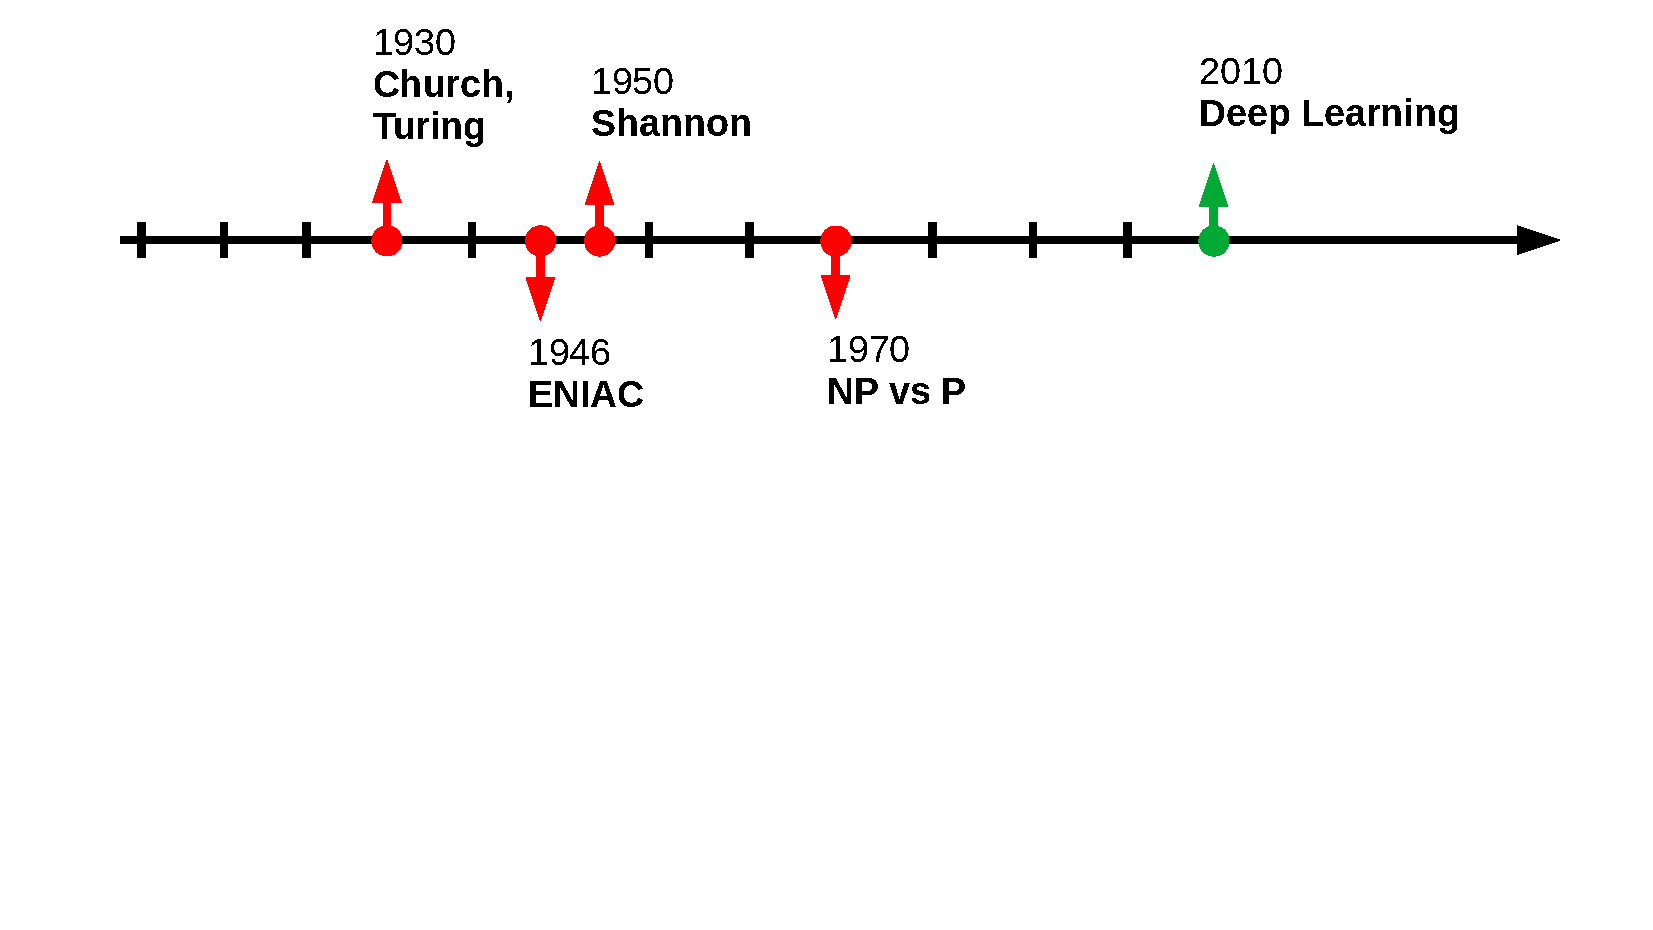
\includegraphics[height=7cm]{figures/t1.pdf}}
      \hspace{-0.175cm}
      \only<2>{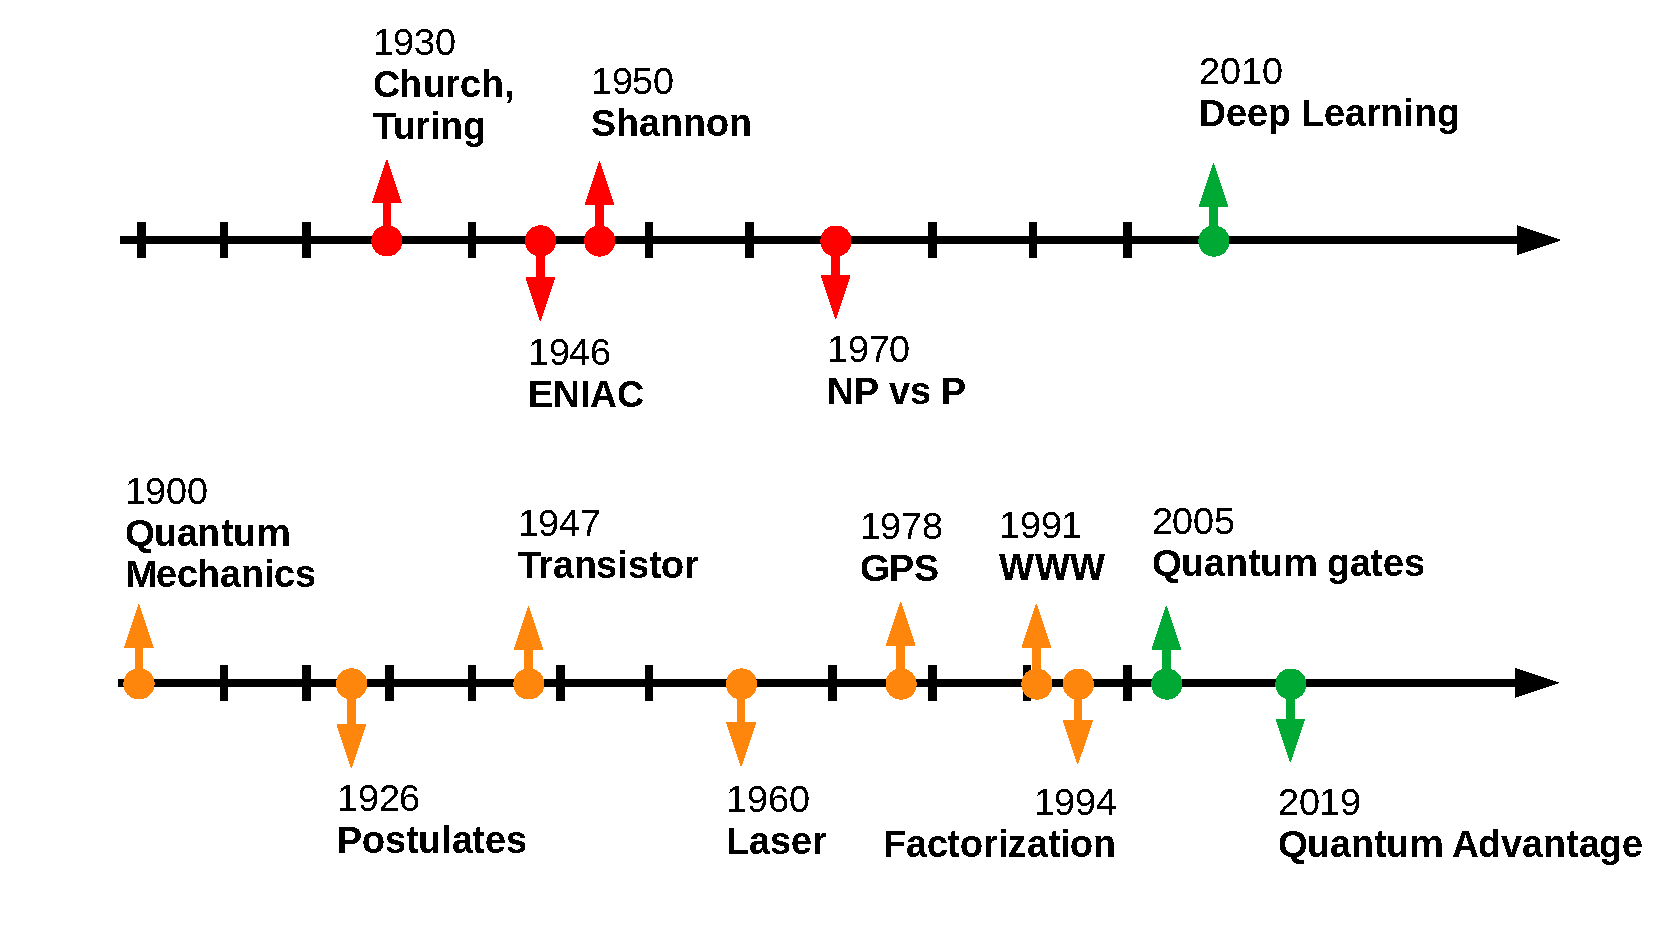
\includegraphics[height=7cm]{figures/t2.pdf}}
      \hspace{-0.23cm}
      \only<3>{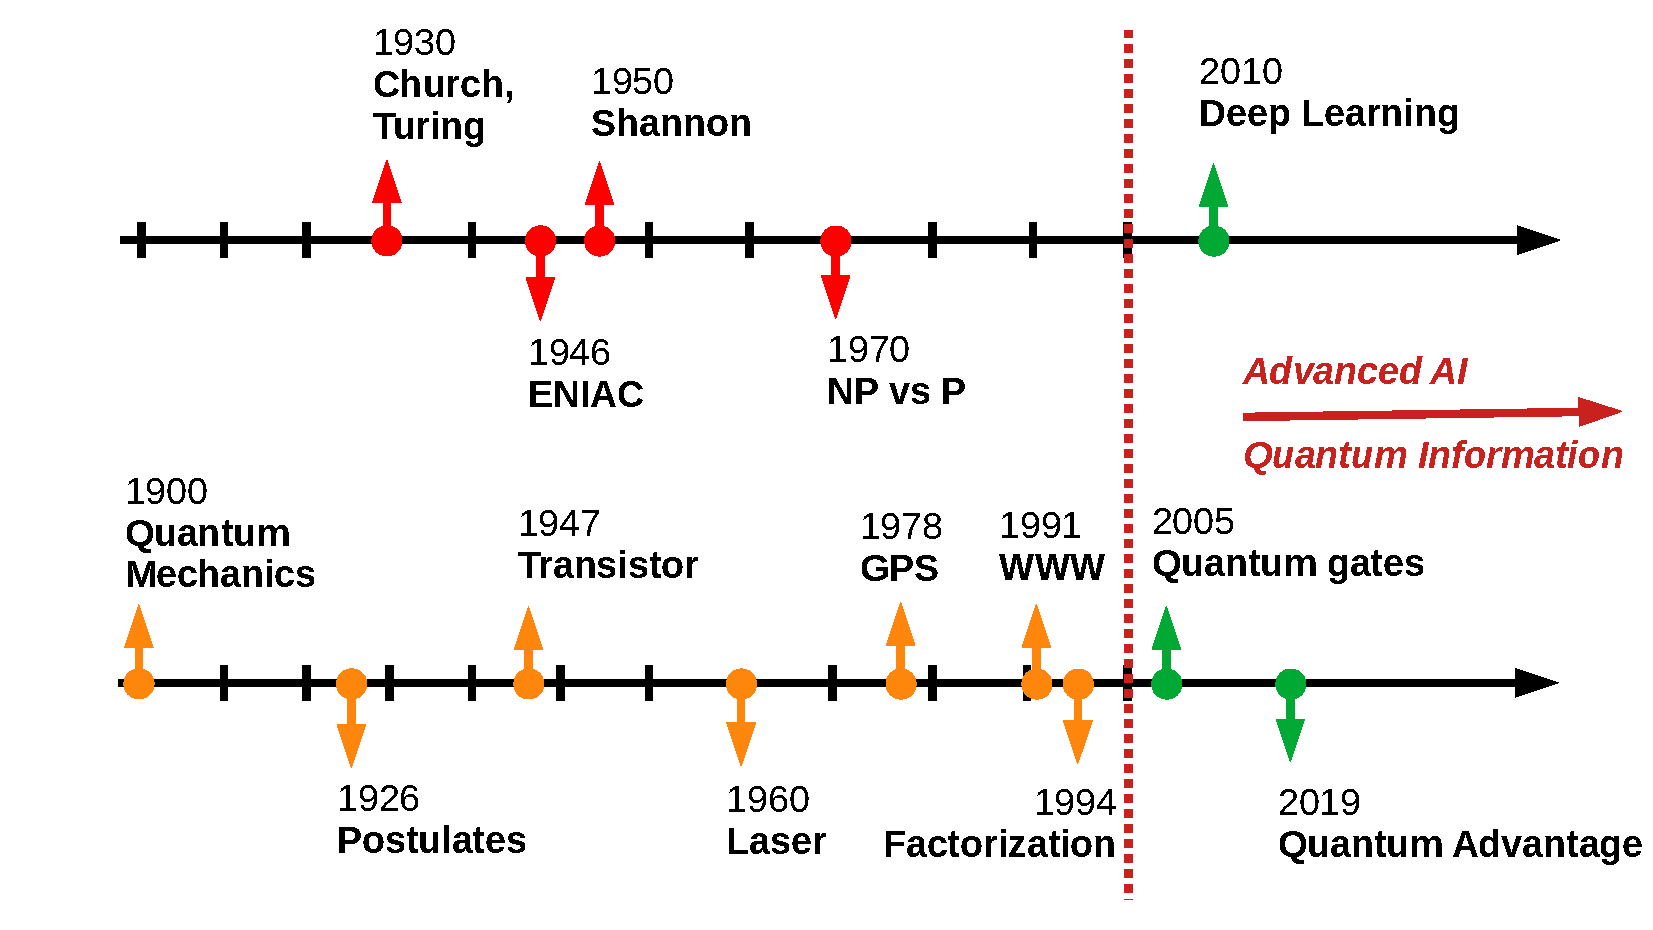
\includegraphics[height=7cm]{figures/t3.pdf}}
   \end{figure}
 \end{frame}

\begin{frame}{R\&D and adoption of new technologies}

   Scientific community is moving towards new technologies, in particular \textbf{\color{blue}hardware
   accelerators}:

   \vspace{-0.5cm}
   \begin{figure}
     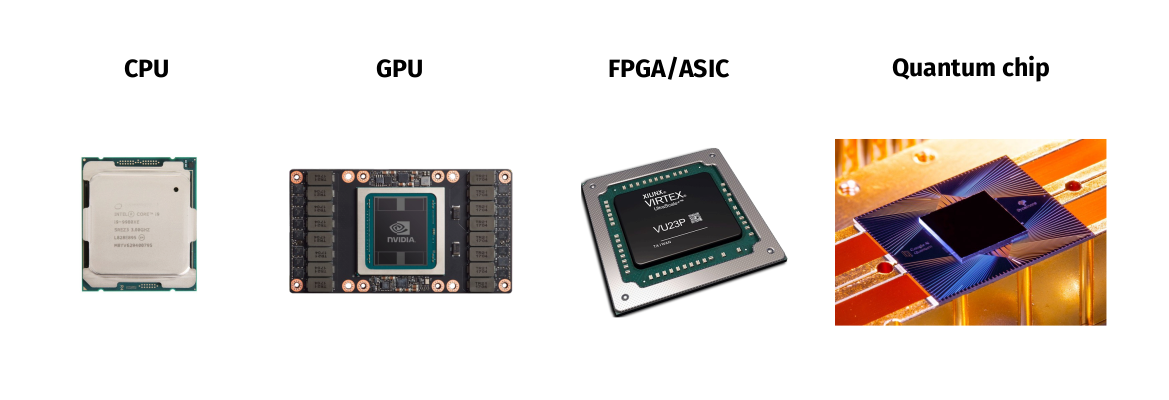
\includegraphics[height=4.5cm]{figures/timeline.png}
   \end{figure}

   \vspace{-1cm}
   \begin{center}
     Moving from \textbf{\color{magenta}general purpose devices} $\Rightarrow$ \textbf{\color{teal}application specific}
   \end{center}

 \end{frame}

 \begin{frame}{Quantum research}

   Structure of research field in {\color{blue}quantum technologies}:
   \begin{figure}
     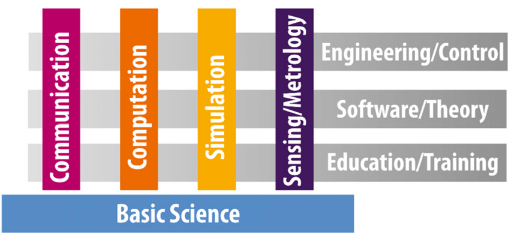
\includegraphics[height=3cm]{figures/rfqt.png}
   \end{figure}

   {\color{blue}Quantum computing} is a paradigm that exploits quantum mechanical properties of
   matter in order to perform calculations.\\
   $\Rightarrow$ Unitary operators, entanglement, superposition, interference, etc.

 \end{frame}

\begin{frame}{Quantum advantage}

   First quantum computation that can not be reproduced on a classical
   supercomputer from Google, {\color{magenta}Nature 574, 505-510(2019)}:

   \begin{figure}
     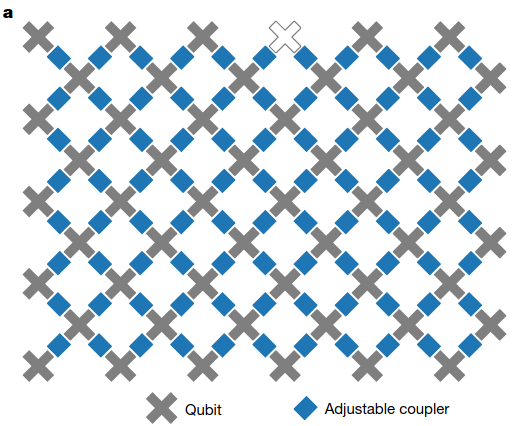
\includegraphics[height=3.2cm]{figures/q3.png}%
     $\quad$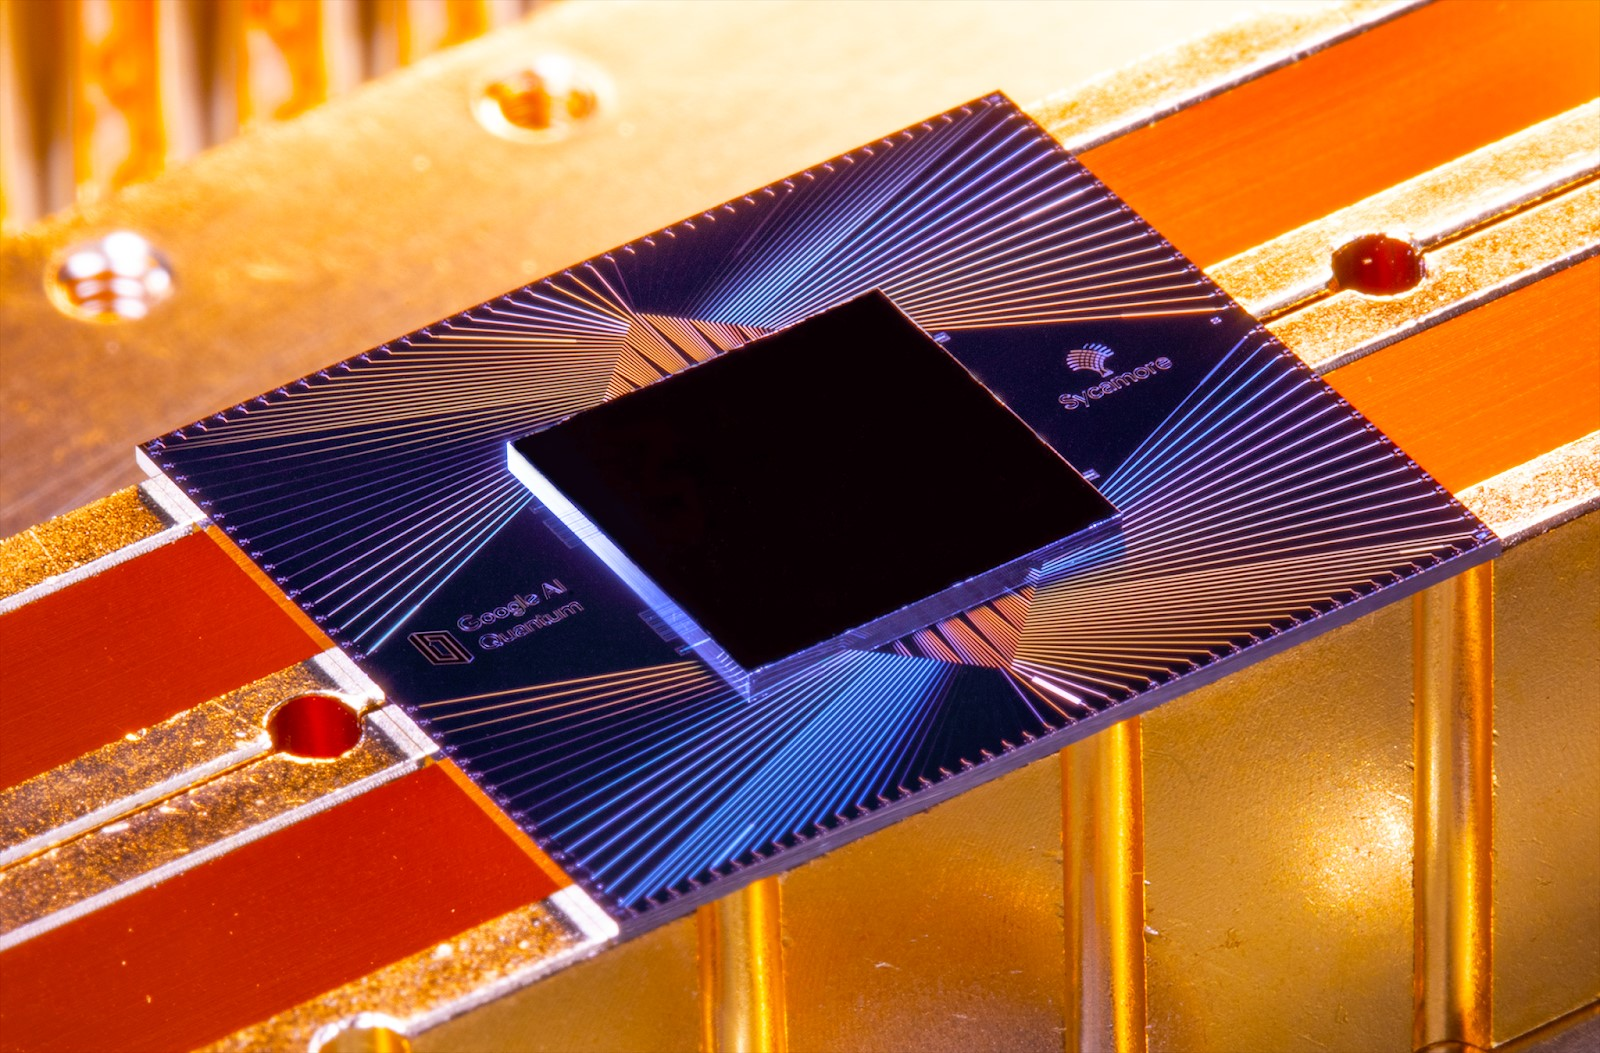
\includegraphics[height=3cm]{figures/q2.png}
   \end{figure}

   \textbf{53 qubits} (86 qubit-couplers) $\rightarrow$ Task of sampling the
   output of a pseudo-random quantum circuit (extract probability
   distribution).

   Classically the probability distribution is {\color{blue}exponentially more difficult}.

 \end{frame}

 \begin{frame}[fragile]{Annual spending on quantum technology}

     \begin{figure}
         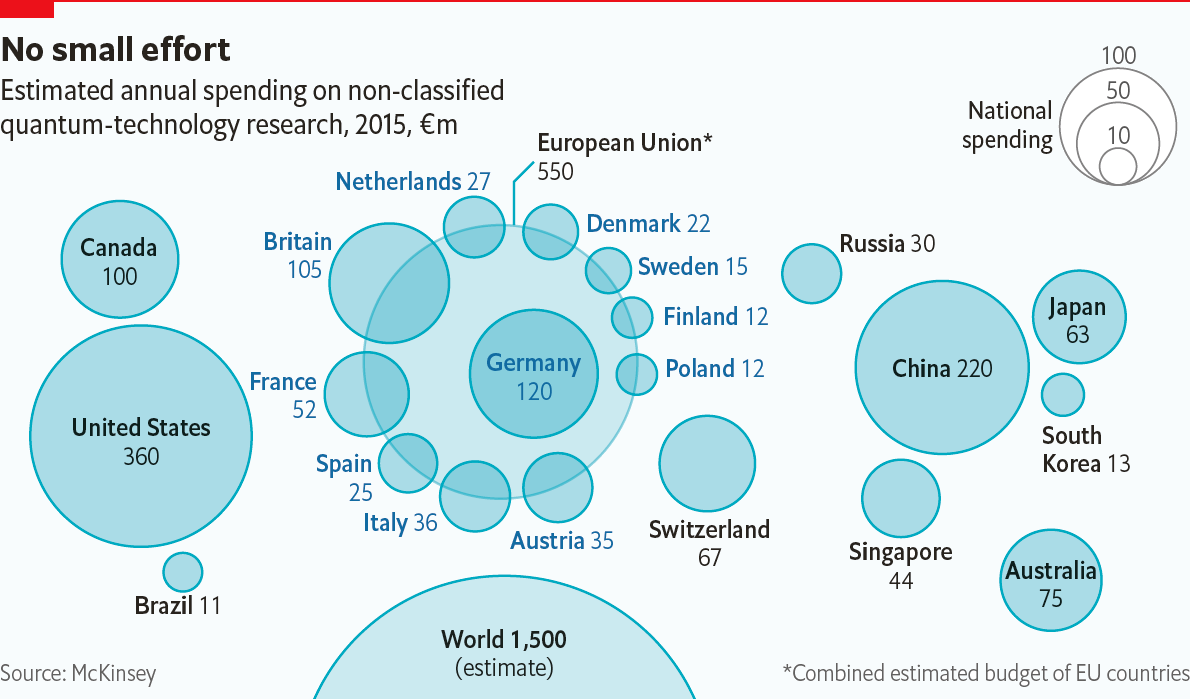
\includegraphics[height=7cm]{figures/20170311_01_DESKTOP.png}
     \end{figure}

 \end{frame}

 \begin{frame}[fragile]{Strong synergy between industry and academics worlds}

     \begin{columns}
         \column{7cm}
     \begin{figure}
         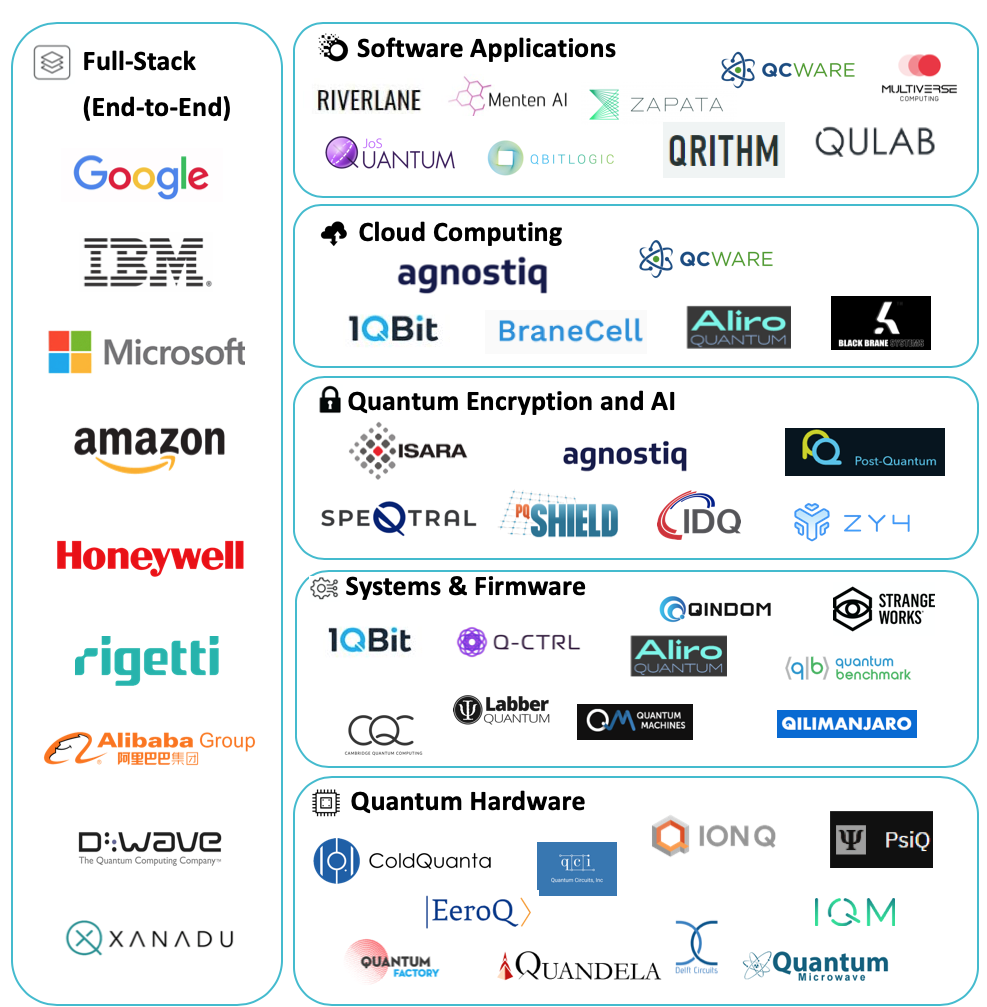
\includegraphics[height=7cm]{figures/companies.png}
     \end{figure}
     \column{7cm}
     \begin{figure}
         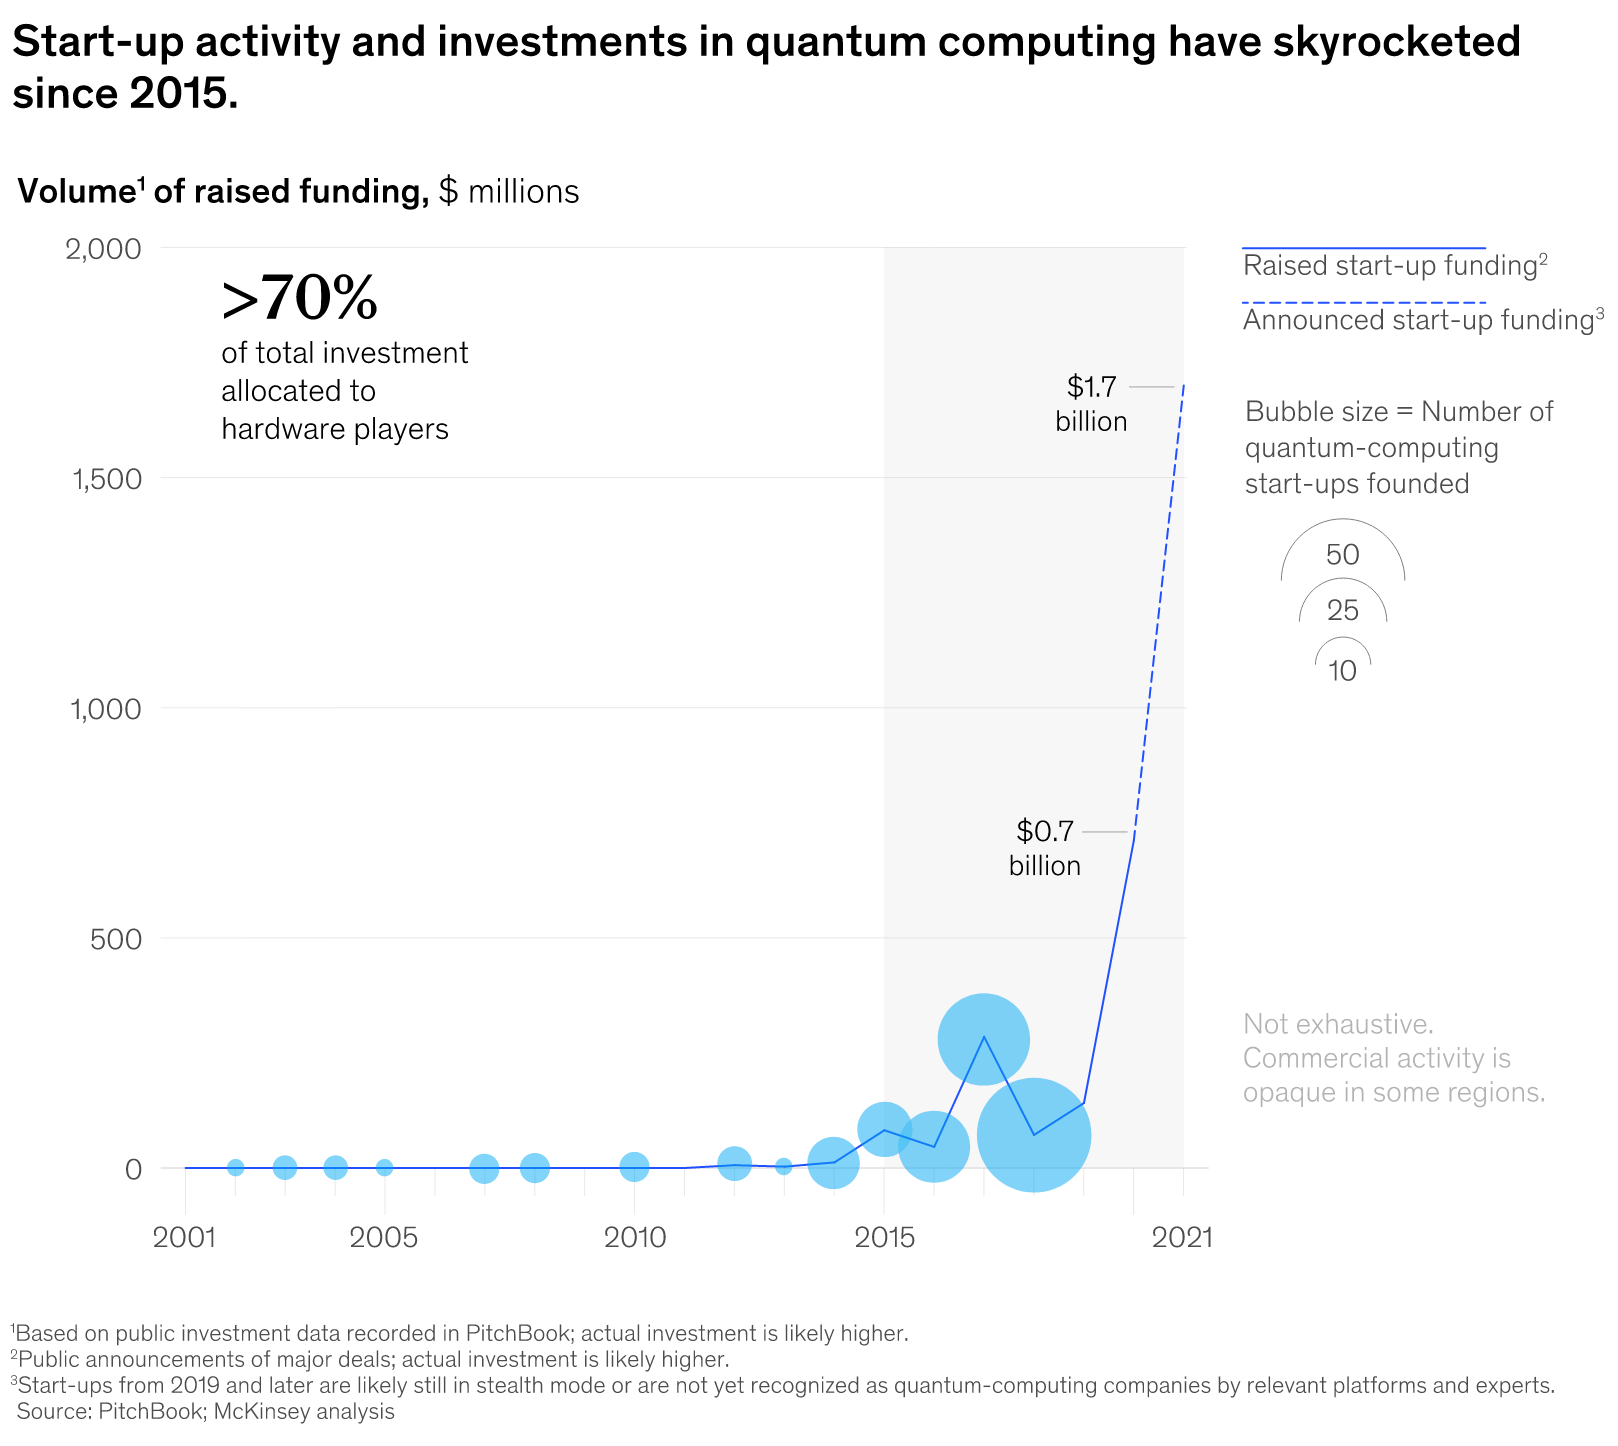
\includegraphics[height=6.5cm]{figures/startup.png}
     \end{figure}
     \end{columns}
 \end{frame}

\section{Quantum Systems}

\begin{frame}{Compute quantum mechanics}
  \pause
  \begin{itemize}[noitemsep]
  \item<2,3>[\faGear] Representing $N$ particles is difficult;
  \item<3>[\faGears] considering $N$ spins ($\uparrow, \downarrow$), we deal with a $2^N$ dimensional Hilbert space!
  \end{itemize}
  %\vspace{0.5cm}
  \begin{multicols}{2}
    \begin{figure}
       \uncover<2,3>{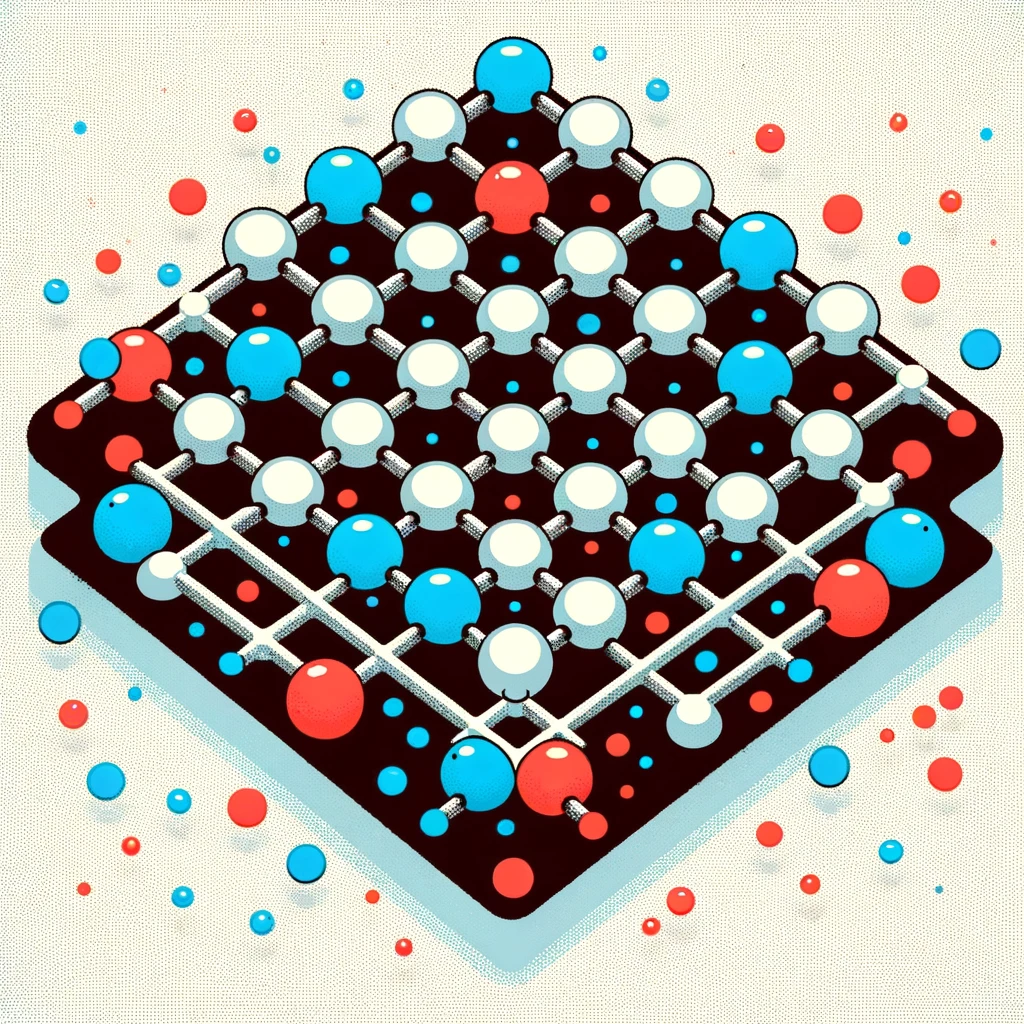
\includegraphics[width=0.4\textwidth]{figures/spins.png}}%
    \end{figure}
    \begin{figure}
       \uncover<3>{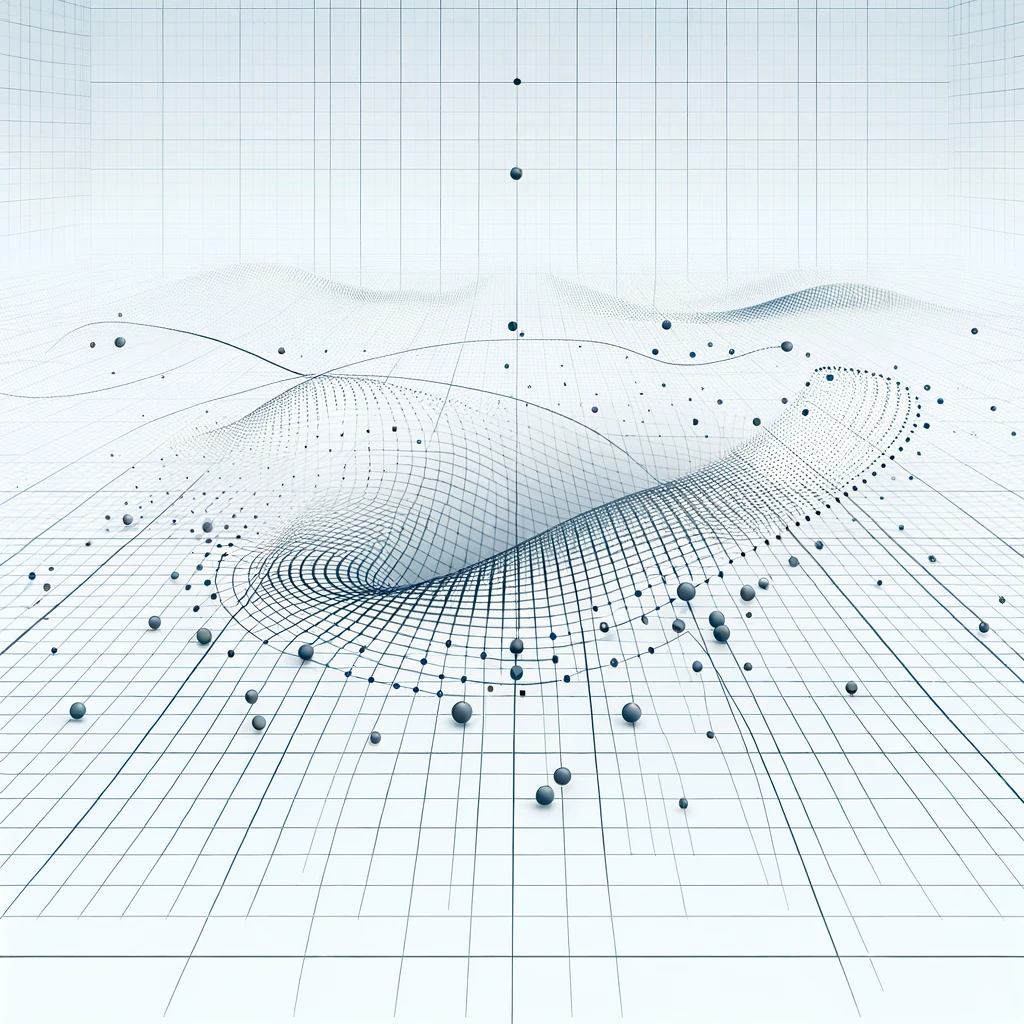
\includegraphics[width=0.4\textwidth]{figures/hilb.png}}%
    \end{figure}
\end{multicols}
\end{frame}

\begin{frame}{What can we do?}
\pause
\begin{itemize}[noitemsep]
\only<2-5>{\item[1.] we can try to use classical methods to represent the system;}
\only<6>{\item[1.] \textbf{\textcolor{amethyst}{we can try to use classical methods to represent the system}};}
\pause
\item[2.] we can build a quantum computer.
\end{itemize}
\pause
\begin{figure}
   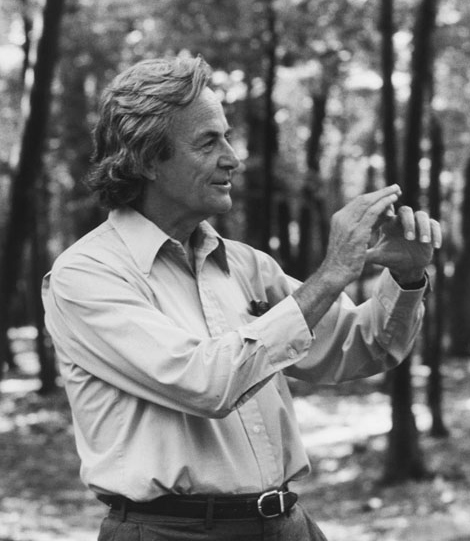
\includegraphics[width=0.3\textwidth, height=0.55\textheight]{figures/feynmann.jpg}%
   $\,\,$ \pause
   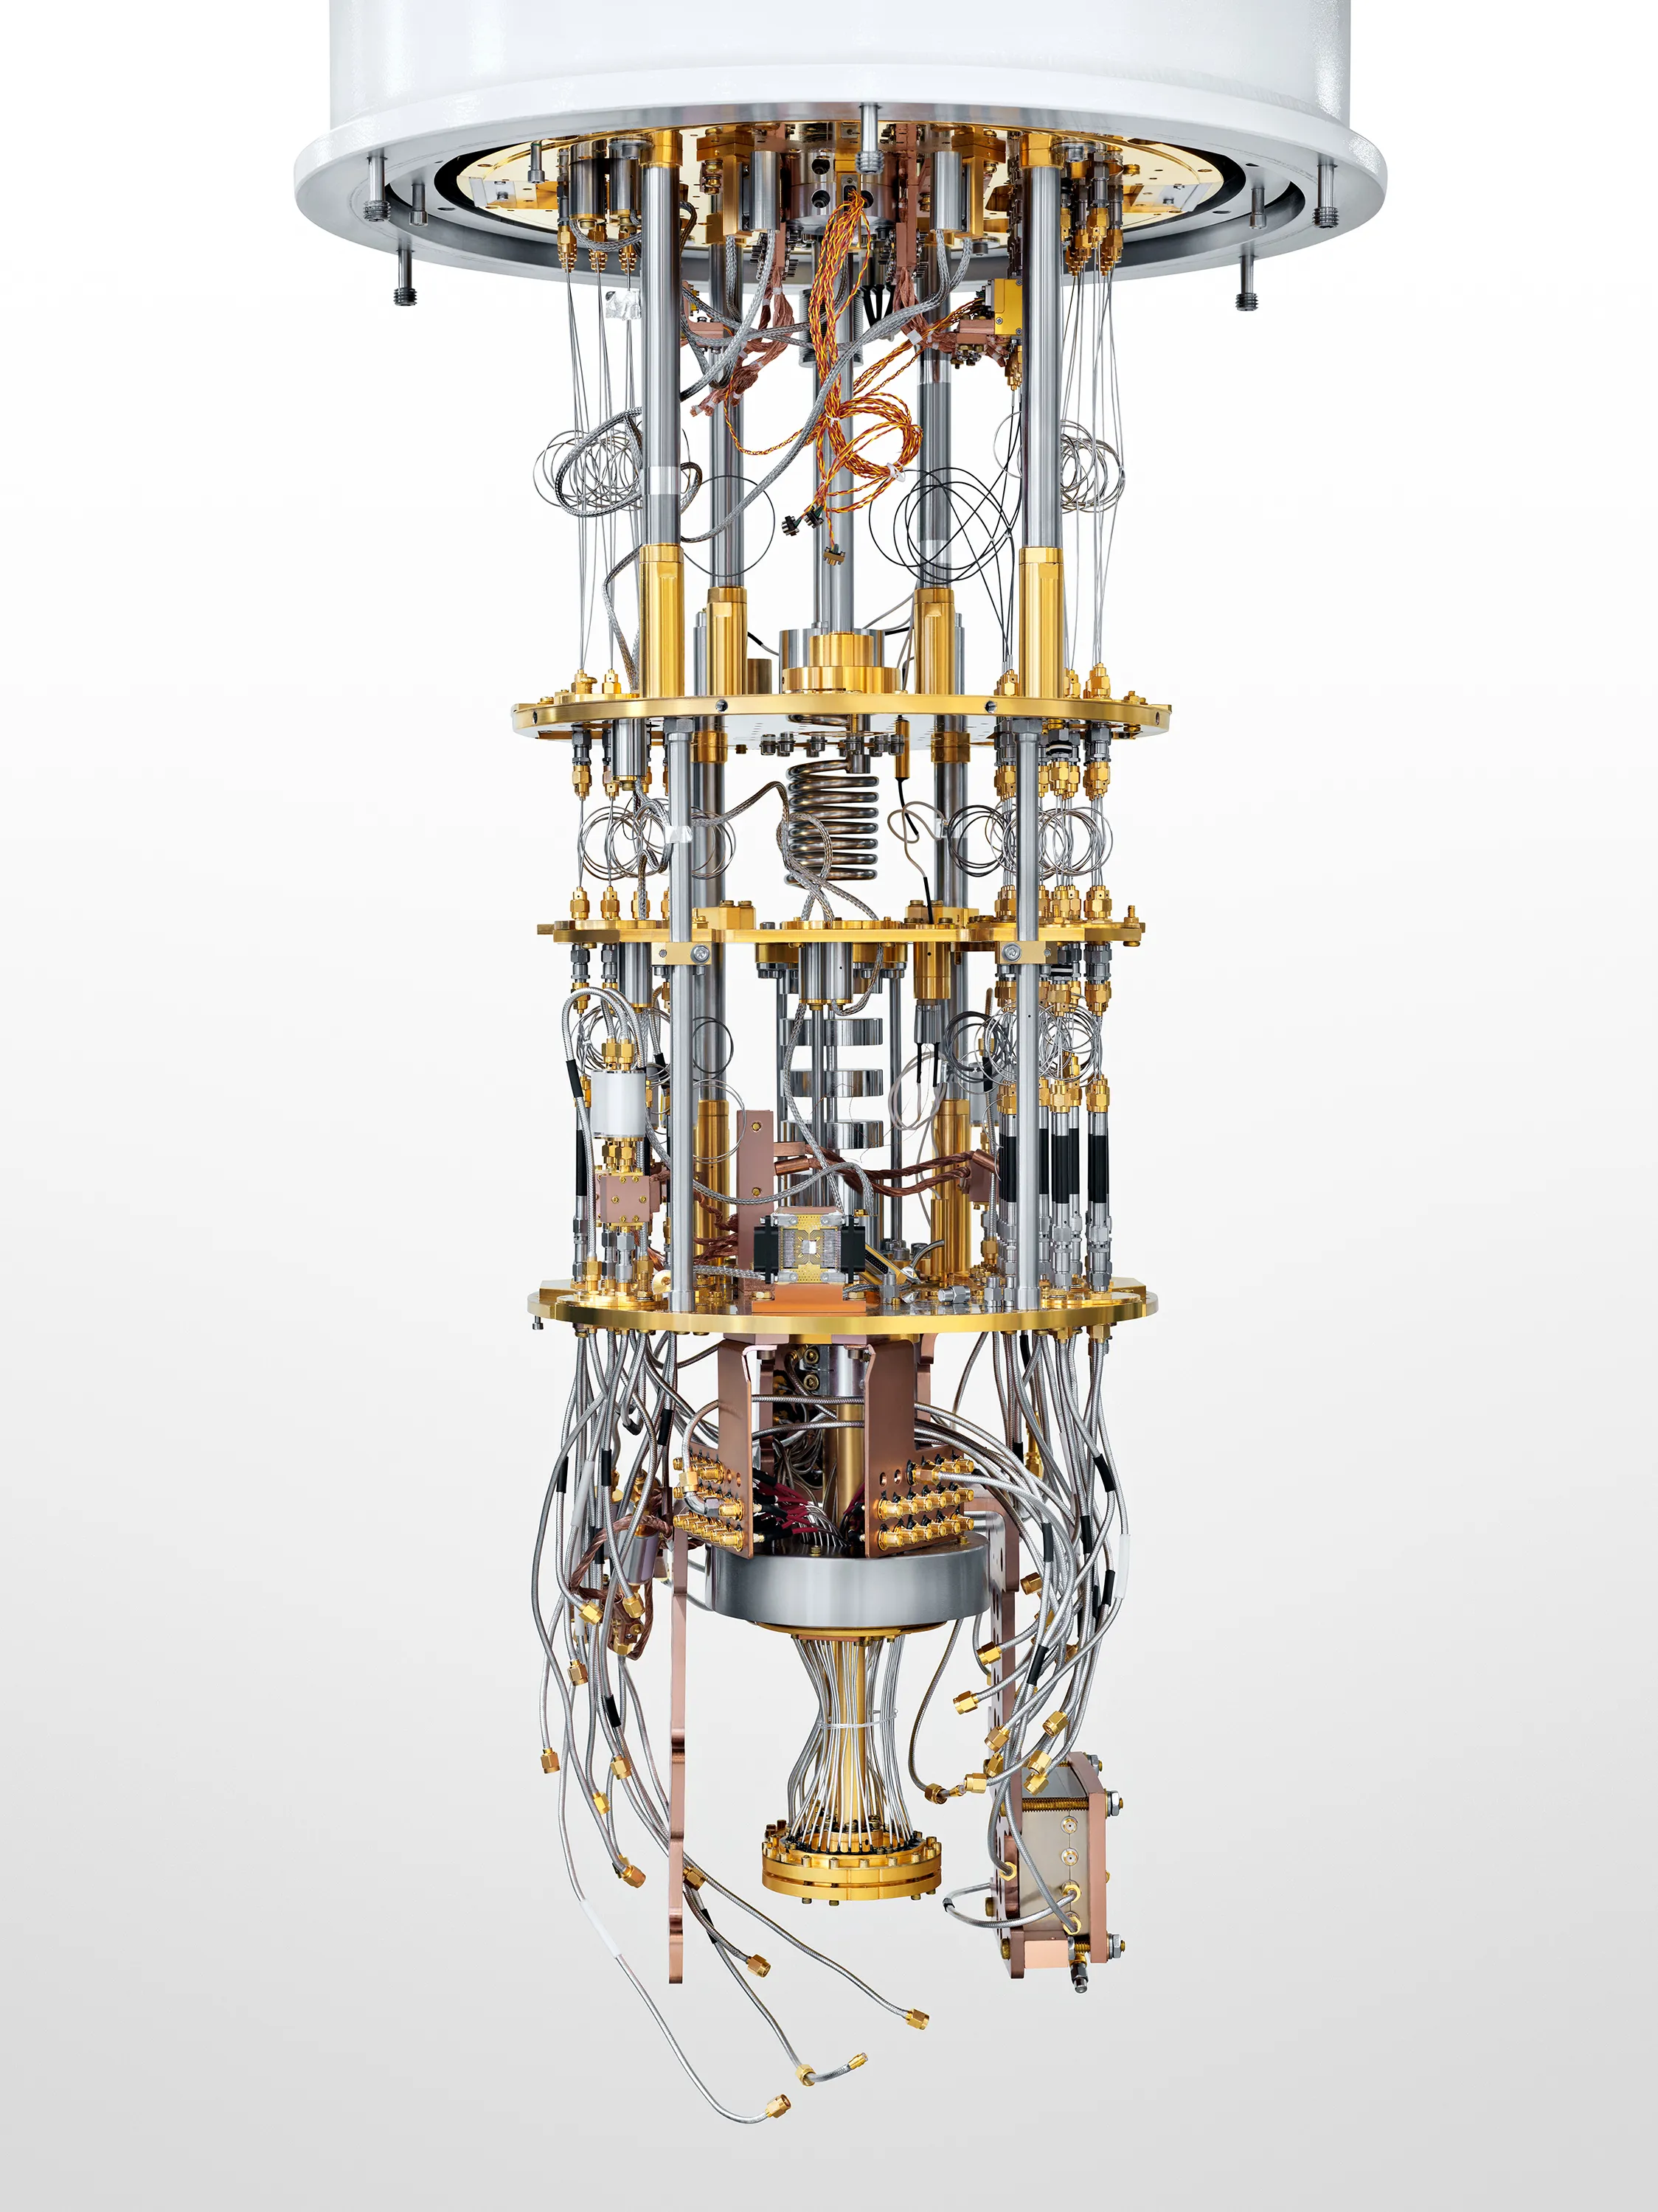
\includegraphics[width=0.3\textwidth, height=0.55\textheight]{figures/qcomp.png}
\end{figure}

\small{ \textit{Nature isn't classical, dammit, and if you want to make a simulation of nature,
you'd better make it quantum mechanical, and by golly it's a wonderful problem,
because it doesn't look so easy.} }

\href{https://link.springer.com/article/10.1007/BF02650179}{\faBook\,\, Richard Feynman, 1982, Simulating Physics with Computers}
\end{frame}


\begin{frame}{Can we represent a state with a classical computer?}
\pause
Let's suppose we want to represent a system of \textbf{qubits} ($\uparrow, \downarrow$).
\pause
\small
\begin{itemize}[noitemsep]
\item[1.] Each \texttt{float 64} requires 8 bytes of memory to be stored;
\pause
\item[2.] each \texttt{complex 128} requires 16 bytes of memory;
\pause
\item[3.] let's take a nice 32Gb of RAM: it can store up to $2$ billions of \texttt{complex 128}.
\pause
\item[4.] a $30$ qubits state requires $\sim 1$ billion of complex numbers;
\pause
\item[5.] a $31$ qubits state cannot be represented by my PC;
\pause
\item[6.] no problem. Let's get serious: \texttt{Fugaku}!
\end{itemize}

\begin{figure}
   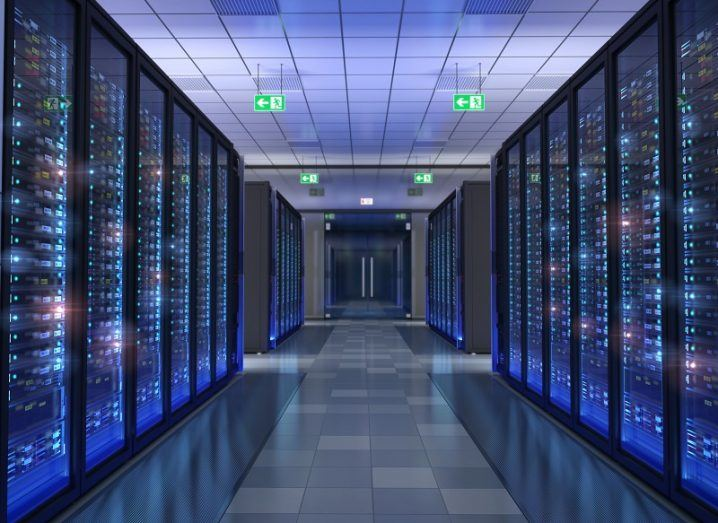
\includegraphics[width=0.42\textwidth, height=0.4\textheight]{figures/fugaku.jpeg}%
   $\,\,$
   \pause
   
\includegraphics[width=0.42\textwidth, height=0.4\textheight]{figures/sad_fugaku.jpg}
\end{figure}
\end{frame}

\begin{frame}{Some smart classical strategies}
   \begin{itemize}[noitemsep]
      \item<2,3,4>[1.] Variational Monte Carlo (VMC): given a wave function $\Psi(\bm{x}|\bm{\theta})$ and a target $H$, MC methods are used to minimize:
      $$ \frac{\int \text{d}\bm{x}\, \Psi^*(\bm{x}|\bm{\theta})\, H \,
      \Psi(\bm{x}|\bm{\theta})}{\int \text{d}\bm{x}\, |\Psi(\bm{x}|\bm{\theta})|^2}\geq E_0; $$
      \item<3,4>[2.] Tensor Networks (TNs): contraction of complex systems into simpler structures;
      \item<4>[3.] Neural Network Quantum States: use complex ANNs to represent the state.
   \end{itemize}
   \begin{multicols}{3}
   \begin{figure}
      \uncover<2,3,4>{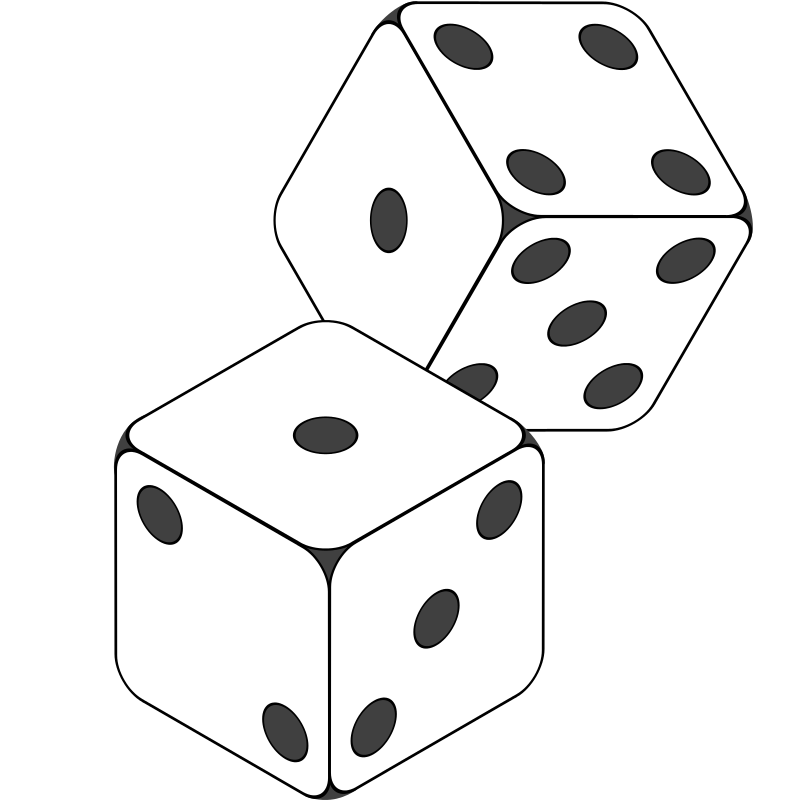
\includegraphics[width=0.7\linewidth, height=0.35\textheight]{figures/dices.png}
      \caption*{\href{https://arxiv.org/abs/1508.02989}{\faBook\,\,arXiv:1508.02989}}}%
      \uncover<3,4>{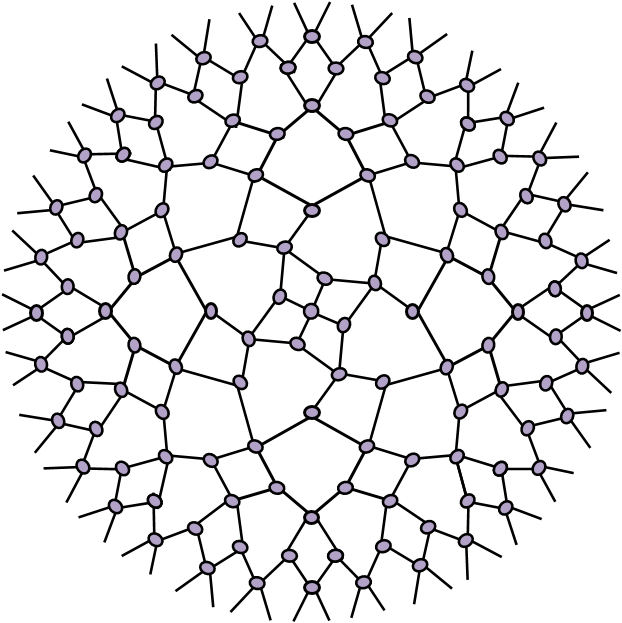
\includegraphics[width=0.7\linewidth, height=0.35\textheight]{figures/tn.png}
      \caption*{\href{https://arxiv.org/abs/1708.00006}{\faBook\,\,arXiv:1708.00006}}}%
      \uncover<4>{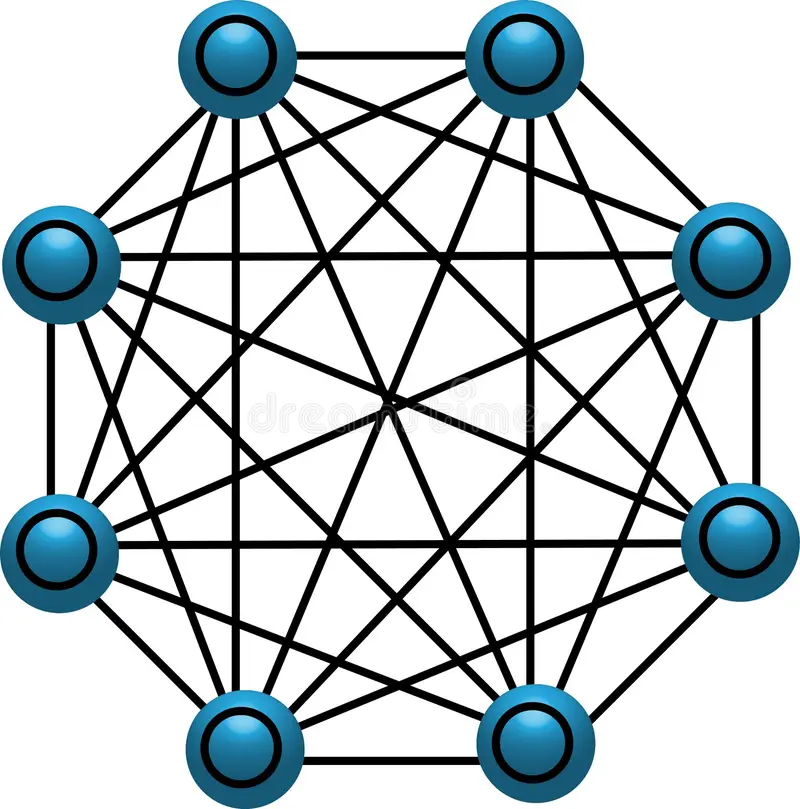
\includegraphics[width=0.7\linewidth, height=0.35\textheight]{figures/bm.png}
      \caption*{\href{https://arxiv.org/abs/1606.02318}{\faBook\,\,arXiv:1606.02318}}}
   \end{figure}
   \end{multicols}
\end{frame}

\begin{frame}{Is this enough? \hfill \href{https://arxiv.org/abs/2103.10293}{\faBook\,\,arXiv:2103.10293}}
\pause
\begin{figure}
   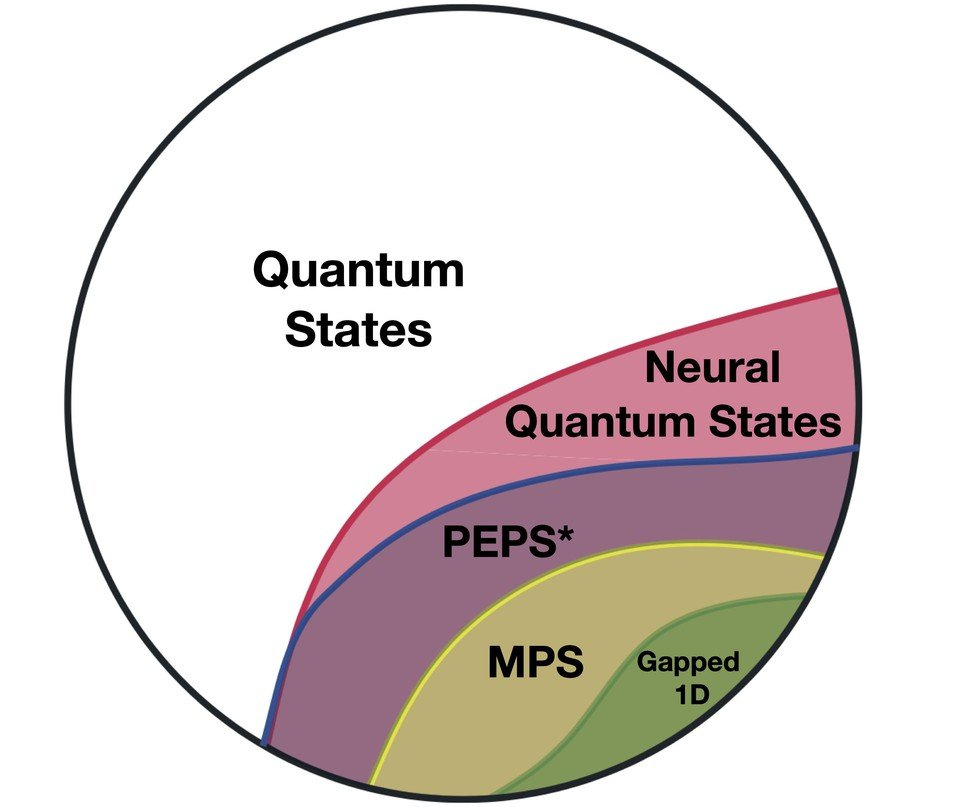
\includegraphics[width=0.6\textwidth]{figures/complexity.jpg}
\end{figure}
\end{frame}

\section{Quantum computing}

\begin{frame}{Qubits}
        \begin{itemize}[noitemsep]
           \item<2,3,4,5>[1.] classical bits are replaced by \textbf{qubits}
           $ \ket{\psi} = \alpha\ket{0}+\beta\ket{1}$.
           \item<3,4,5>[2.] we can manipulate the qubit state applying \textbf{gates}: $\ket{\psi'}=\mathcal{U}(\bm{\theta})\ket{\psi}.$

           Typically we use 1-qubit and 2-qubits gates!
         %   $$ H \ket{0} = \frac{\ket{0}+\ket{1}}{\sqrt{2}} \qquad \text{with}\qquad  H =
         %   \begin{pmatrix}
         %   1 & 1 \\ 1 & -1
         %   \end{pmatrix}.
         %   $$
           \item<4,5>[3.] combine together gates to build \textbf{quantum circuits};
           \item<5>[4.] to access the information we need to measure the system.
        \end{itemize}
        \begin{figure}
            \only<2>{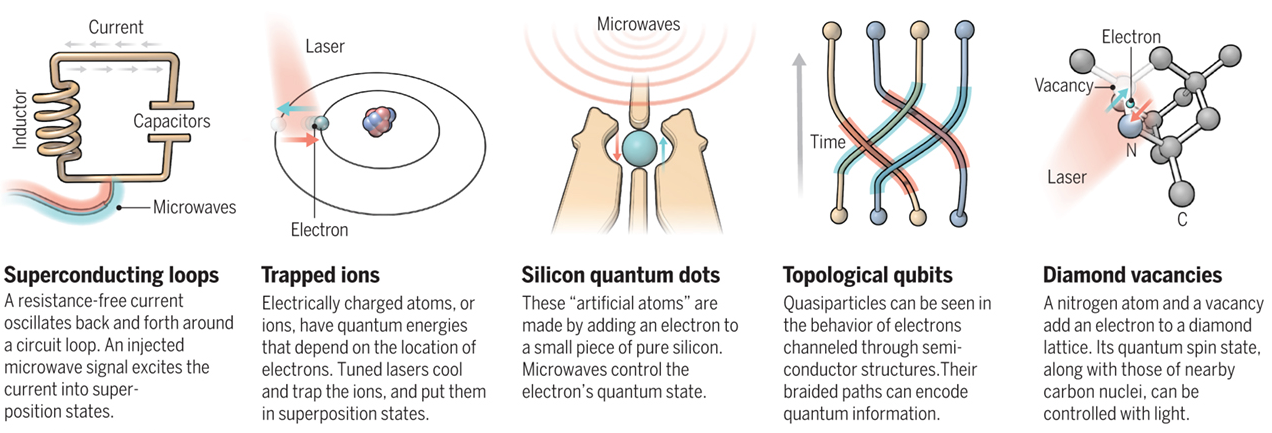
\includegraphics[width=0.8\linewidth, height=0.45\textheight]{figures/qubits.png}}%
            \only<3>{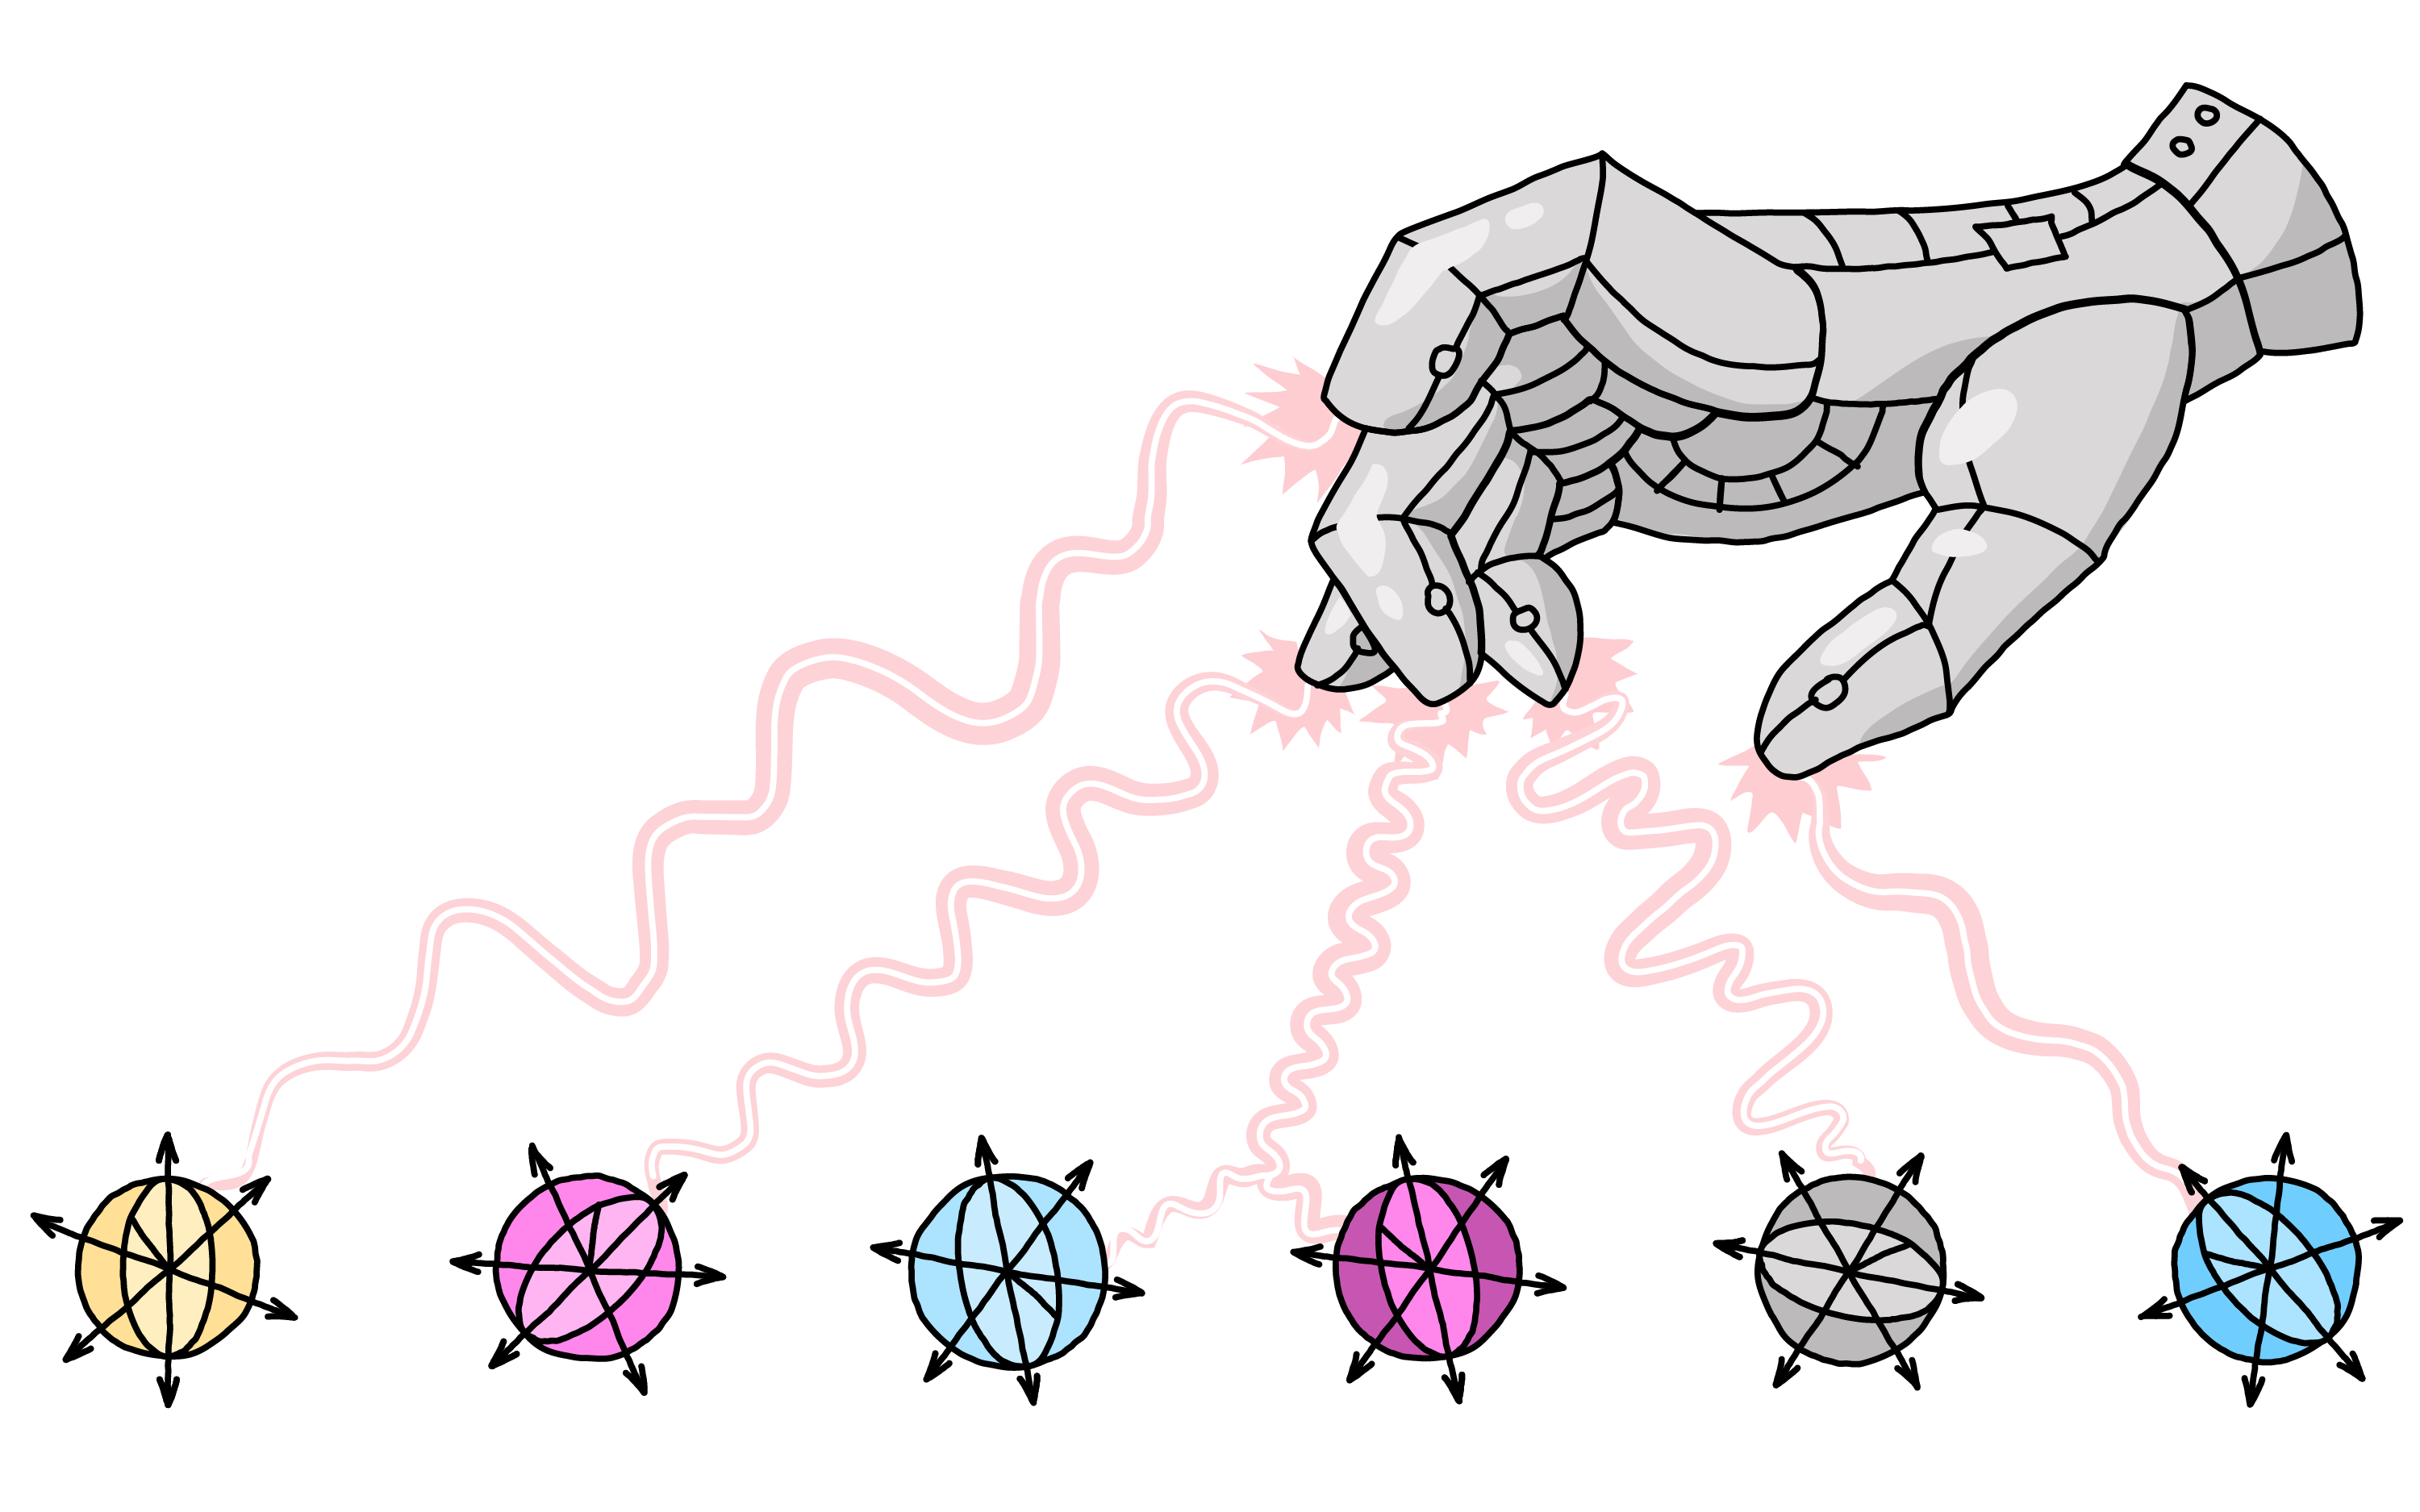
\includegraphics[width=0.45  \linewidth, height=0.45\textheight]{figures/pulses.png}}%
            \only<4>{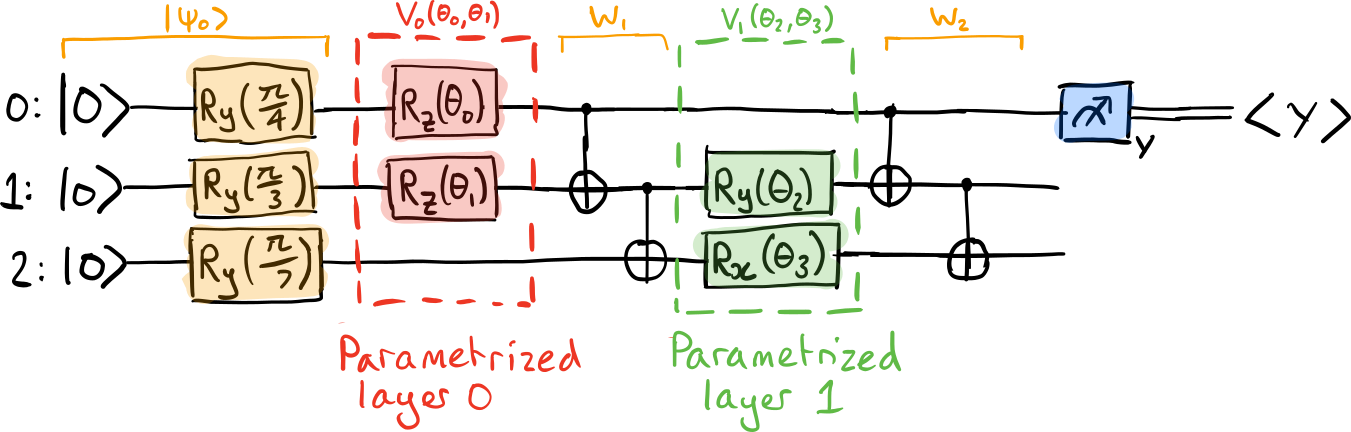
\includegraphics[width=0.9\linewidth, height=0.45\textheight]{figures/circuit.png}}
            \only<5>{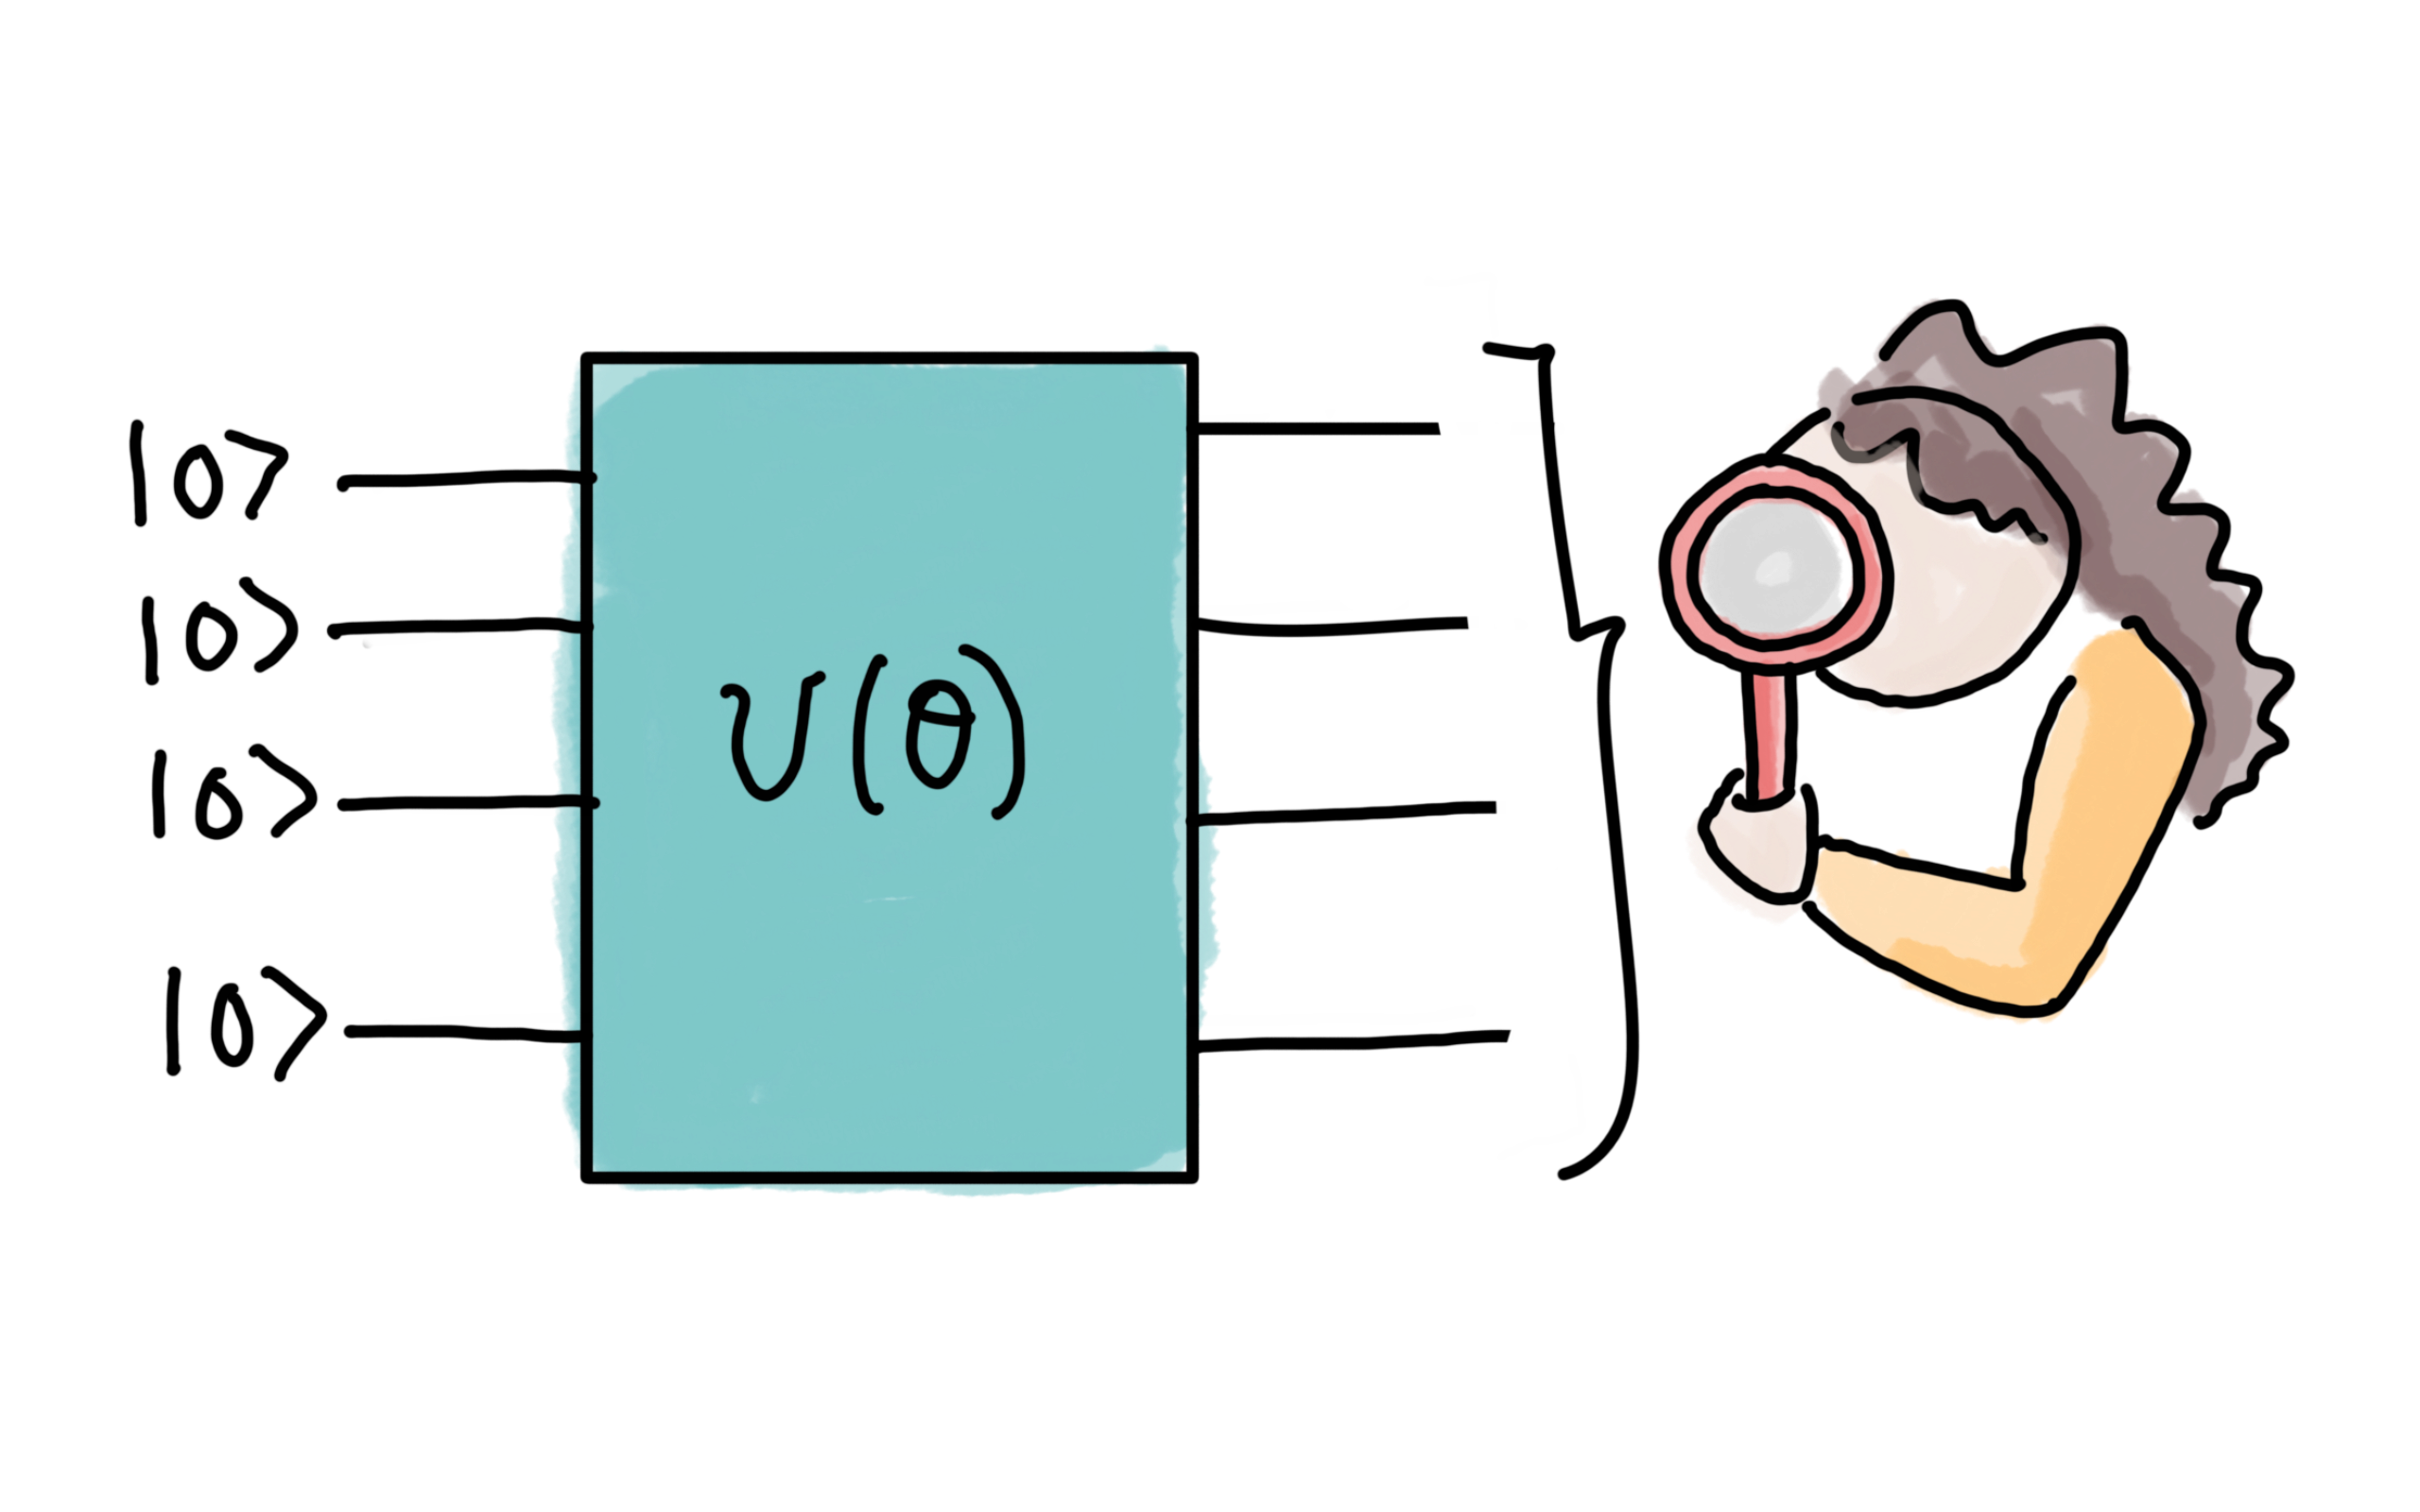
\includegraphics[width=0.5\linewidth, height=0.45\textheight]{figures/measurement.png}}
        \end{figure}
\end{frame}

\begin{frame}[fragile]{What is a qubit?}
   \pause
   Let us consider a two-dimensional {\color{blue}Hilbert space}, we define the computational basis:
   \begin{equation*}
   \ket{0} \rightarrow  \begin{bmatrix} 1 \\ 0 \end{bmatrix}, \qquad \qquad
   \ket{1} \rightarrow  \begin{bmatrix} 0 \\ 1 \end{bmatrix}.
   \end{equation*}

   A {\color{red}quantum bit} (\textbf{qubit}) is the basic unit of quantum information and it is written as:
   \begin{equation*}
   \ket{\psi}=\alpha\ket{0} +\beta\ket{1},
   \end{equation*}
   where $\alpha, \beta$ are {\color{violet}complex numbers} and the {\color{blue}state is normalized}, i.e. $|\alpha|^2+|\beta|^2=1$.

   %All quantum mechanics rules are preserved: state measurement is probabilistic,
   %wave-function collapse after measurement, no-cloning theorem, etc.

 \end{frame}

 \begin{frame}[fragile]{Multiple qubits states}

 A system with $n$ qubits lives in {\color{red}$2^n$-dimensional Hilbert space}, defining the basis:
 \begin{equation*}
 \ket{0}_n = \ket{00\dots0 0},\, \ket{1}_n = \ket{00\dots01},\, \ket{2}_n = \ket{00\dots10}, \, \dots, \ket{2^n -1}_n = \ket{11\dots1}
 \end{equation*}
 therefore a generic $n$ qubits state is defined as
 \begin{equation*}
 \ket{\psi_n}= \sum_{i=0}^{2^n-1} \alpha_i \ket{i}_n \quad \text{with } \quad  \sum_{i=0}^{2^n-1} |\alpha_i |^2 = 1
 \end{equation*}
 \textit{i.e.} a {\color{blue}superposition state vector} with \textbf{$2^n$ complex numbers}.

 \end{frame}


\begin{frame}{Quantum circuits}

   The {\color{blue}quantum circuit} model considers a sequence of unitary quantum gates:
   \begin{equation*}
     \ket{\psi'} = U_2 U_1 \ket{\psi} \quad \rightarrow \quad \quad
     \Qcircuit @C=1em @R=.7em {
       \ket{\psi} & & \gate{U_1} & \gate{U_2} & \qw & \ket{\psi'}
       }
   \end{equation*}

   The final state $|\psi'\rangle$ is given by:
   \vspace{0.2cm}
   \begin{equation*}
       \psi '(\boldsymbol{\sigma }) = \sum _{\boldsymbol{\sigma '}} {\color{blue} U_1 U_2(\boldsymbol{\sigma }, \boldsymbol{\sigma '})} {\color{red}\psi (\sigma _1,\dots \sigma _{i_1}',\dots ,\sigma _{i_{N_\mathrm{targets}}}', \dots , \sigma _N ) },
   \end{equation*}
   where the sum runs over qubits targeted by the gate.
   \begin{itemize}
     \item {\color{blue}$U_2$} and {\color{blue}$U_1$} are gate matrices which act on the state vector.
     \item {\color{red}$\psi$} is a state and it is bounded by memory.
   \end{itemize}

 \end{frame}

\begin{frame}{Quantum gates}

   \begin{columns}

     \column{6cm}
     \begin{itemize}
       \item {\bf Single-qubit gates}
       \begin{itemize}
         \item Pauli gates
         \item Hadamard gate
         \item Phase shift gate
         \item Rotation gates
       \end{itemize}
       \item {\bf Two-qubit gates}
       \begin{itemize}
         \item Controlled gates
         \item Swap gate
         \item fSim gate
       \end{itemize}
       \item \textbf{Three-qubit gates}
       \begin{itemize}
         \item Toffoli
       \end{itemize}
     \end{itemize}

     \column{6cm}
     \begin{figure}
       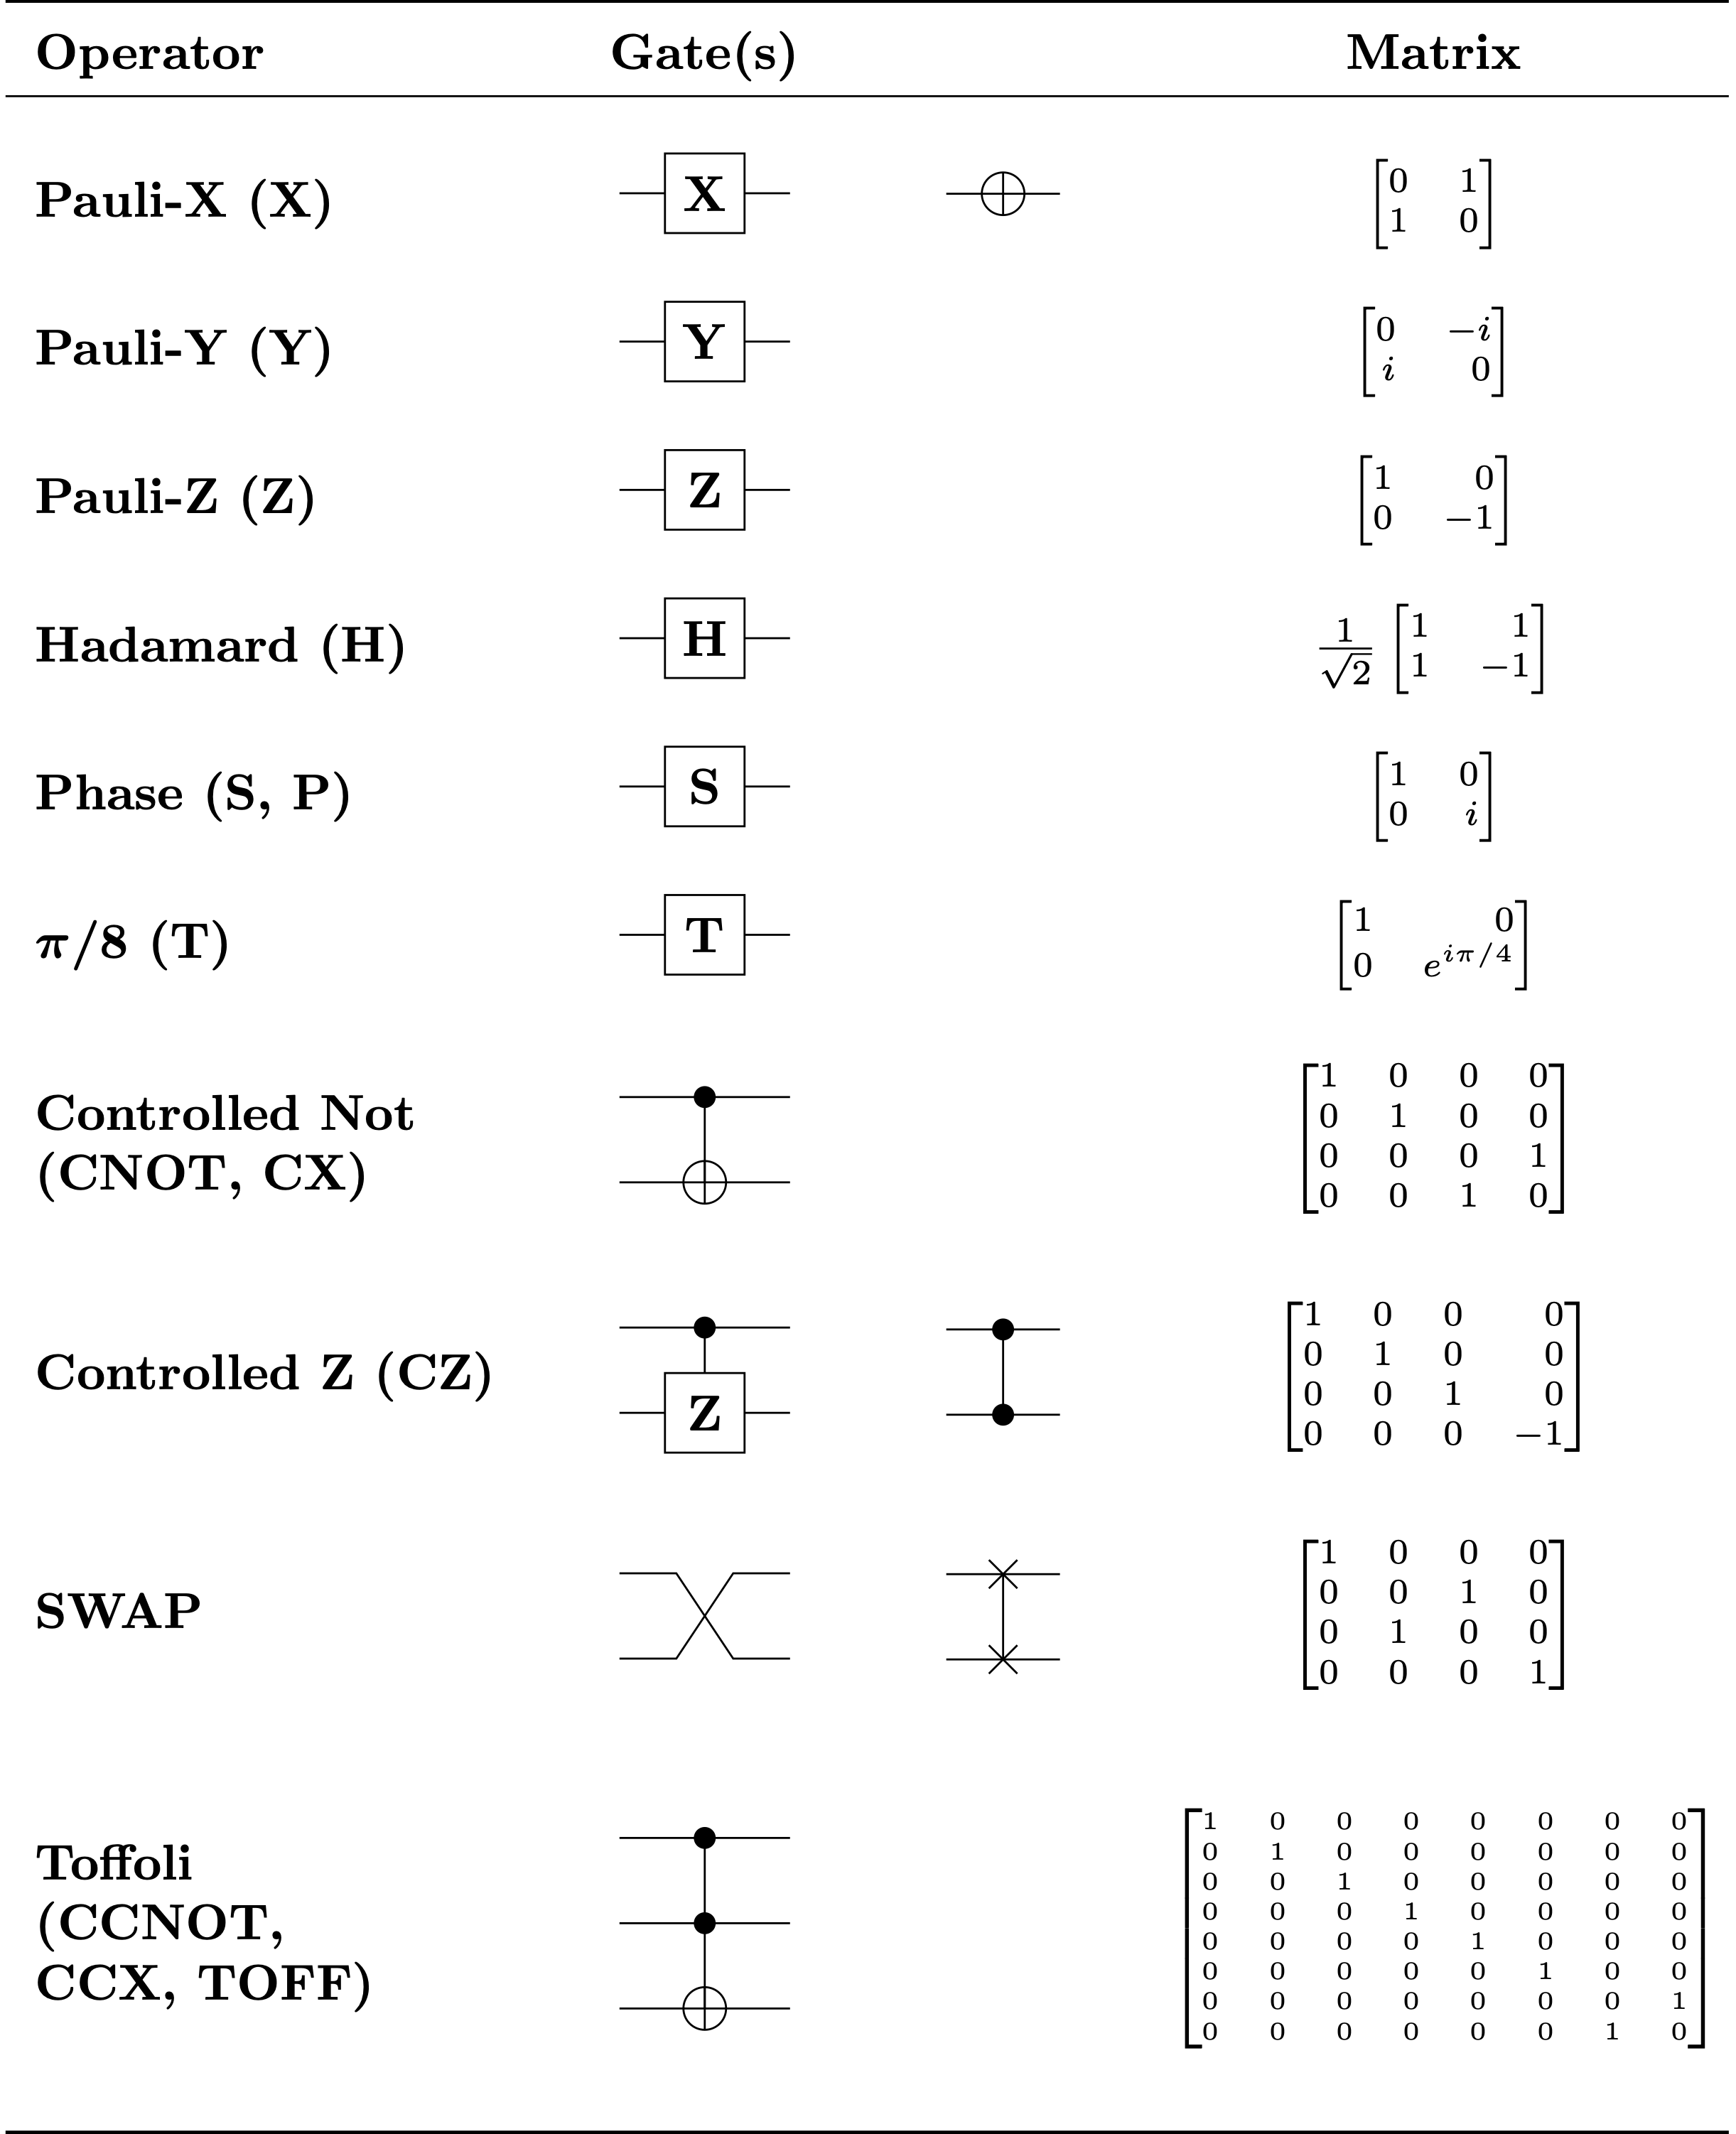
\includegraphics[height=7cm]{figures/Quantum_Logic_Gates.png}
     \end{figure}

   \end{columns}

 \end{frame}

 \begin{frame}{Pauli gates}

   \begin{columns}
     \column{7cm}
     \metroset{block=fill}
     \begin{block}{$X$ gate}
     The $X$ gate acts like the classical NOT gate, it is represented by the
     $\sigma_x$ matrix,
     \begin{equation*}
       \sigma_x= \begin{bmatrix} 0 & 1  \\ 1 & 0\end{bmatrix}
     \end{equation*}
     therefore
     \begin{equation*}
       \Qcircuit @C=1em @R=.7em {
         \ket{0} & & \gate{X} & \qw & \ket{1}
         }
     \end{equation*}
     \begin{equation*}
         \Qcircuit @C=1em @R=.7em {
           \ket{1} & & \gate{X} & \qw & \ket{0}
         }
     \end{equation*}
   \end{block}
   \column{7cm}
   \metroset{block=fill}
   \begin{alertblock}{$Z$ gate}
   The $Z$ gate flips the sign of $\ket{1}$, it is represented by the $\sigma_z$
   matrix,
   \begin{equation*}
     \sigma_z= \begin{bmatrix} 1 & 0  \\ 0 & -1 \end{bmatrix}
   \end{equation*}
   therefore
   \begin{equation*}
     \Qcircuit @C=1em @R=.7em {
       \ket{0} & & \gate{Z} & \qw & \ket{0}
       }
   \end{equation*}
   \begin{equation*}
       \Qcircuit @C=1em @R=.7em {
         \ket{1} & & \gate{Z} & \qw & \quad -\ket{1}
       }
   \end{equation*}
 \end{alertblock}

 \end{columns}

 \end{frame}

\begin{frame}{Hadamard gate}

   The Hadamard gate ($H$ gate) is defined as
   \begin{equation*}
     H = \frac{1}{\sqrt{2}}
     \begin{bmatrix}
         1 & 1  \\
         1 & -1
     \end{bmatrix}
   \end{equation*}

   Therefore it creates a superposition of states
   \begin{equation*}
     \Qcircuit @C=1em @R=.7em {
       \ket{0} & & \gate{H} & \qw &
     }
     \frac{\ket 0+\ket 1}{\sqrt 2} \equiv \ket +
   \end{equation*}
   \begin{equation*}
     \Qcircuit @C=1em @R=.7em {
       \ket{1} & & \gate{H} & \qw &
     }
     \frac{\ket 0-\ket 1}{\sqrt 2} \equiv \ket -
   \end{equation*}

   \end{frame}

 \begin{frame}{Measurements}

   In real experiments we perform measurements with a preselected number of shots.

   Shots contribute to the reconstruction of the underlying wave-function distribution.

   \metroset{block=fill}
   \begin{alertblock}{Measurement ($M$) gate:}
     Lets consider the following circuit:
   \begin{equation*}
     \Qcircuit @C=1em @R=.7em {
       \ket{0} & & \gate{H} & \qw & \meter
     }
   \end{equation*}
   The analytic final state is:
   \begin{equation*}
     \frac{\ket{0}+\ket{1}}{\sqrt{2}}
   \end{equation*}
   When measuring the final state we obtain 0 or 1 each with 50\% probability.
   \end{alertblock}

 \end{frame}

\begin{frame}{New computational power: an example}
\pause
With quantum computing, we introduce new tools.
\pause
\begin{itemize}[noitemsep]
\item[\faRocket] prepare a quantum state in the computational zero $\ket{0}$;
\pause
\item[\faSliders] we can prepare superposition:
$$H\ket{0} = \frac{1}{\sqrt{2}}(\ket{0} + \ket{1}) \pause \quad \text{with} \quad H = \frac{1}{\sqrt{2}}
\begin{bmatrix} 1 & 1 \\ 1 & -1 \end{bmatrix},\,\, \ket{0}=\begin{bmatrix} 1 \\ 0
\end{bmatrix},\,\,\ket{1}=\begin{bmatrix} 0 \\ 1 \end{bmatrix};$$
\pause
\item[\faShareAlt] let's apply a controlled-NOT (CNOT) gate on a second qubit prepared in $\ket{0}$:
$$ \text{CNOT} \biggl( \underbrace{\frac{1}{\sqrt{2}}(\ket{0} + \ket{1})}_{\text{control}}\otimes
\ket{0} \biggr) = \pause \frac{1}{\sqrt{2}}(\ket{\textcolor{bleudefrance}{0}0} +
\text{NOT}_{\rm targ}\ket{\textcolor{brightmaroon}{1}0}) = \pause \frac{1}{\sqrt{2}}(\ket{00} + \ket{11}). $$
\end{itemize}
\pause
\vspace{-0.5cm}
\begin{figure}
   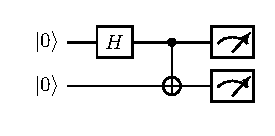
\includegraphics[width=0.4\linewidth]{figures/baby3.pdf}
\end{figure}
\end{frame}

\begin{frame}{Parametric gates prepare variational quantum states}
\pause
\begin{itemize}[noitemsep]
\item[\faLightbulbO] Among the gates, parametric ones can be useful!
\pause
\item[\faMapPin] Let's consider a single qubit system:
\begin{equation*}
   \ket{\psi} = \alpha\ket{0}+\beta\ket{1} \qquad \pause \text{with}
   \qquad \alpha = \cos{\frac{\theta}{2}}, \quad \beta = e^{i\phi}\sin{\frac{\theta}{2}}.
\end{equation*}
\end{itemize}
\vspace{-0.7cm}
\begin{center}
\begin{multicols}{2}
\def\rotationSphere{-110}
\def\radiusSphere{1.8cm}
\def\psiLat{45}
\def\psiLon{45}
\begin{blochsphere}[radius=\radiusSphere,opacity=0,rotation=\rotationSphere]
  % \drawBallGrid[style={opacity=.3}]{30}{45}
  % Draw the sphere...
  \drawLongitudeCircle[]{\rotationSphere}

  \drawLatitudeCircle[style={dashed}]{0}
  % Define the different points on the bloch sphere
  \labelLatLon{ket0}{90}{0};
  \labelLatLon{ket1}{-90}{0};
  \labelLatLon{ketminus}{0}{180};
  \labelLatLon{ketplus}{00}{0};
  \labelLatLon{ketpluspi2}{0}{-90};  % Longitude seems to be defined in the "wrong" direction, hence the minus
  \labelLatLon{ketplus3pi2}{0}{-270};
  \labelLatLon{psi}{\psiLat}{-\psiLon};
  % Draw and label the axis
  \draw[-latex] (0,0) -- (ket0) node[above,inner sep=.5mm] at (ket0) {\footnotesize $z$};
  \draw[-latex] (0,0) -- (ketplus) node[below,inner sep=.5mm] at (ketplus) {\footnotesize$x$};
  \draw[-latex] (0,0) -- (ketpluspi2) node[below,inner sep=.5mm] at (ketpluspi2) {\footnotesize $y$};
  % Draw |psi>
  \draw[-latex] (0,0) -- (psi) node[above]{\footnotesize $\ket{\psi}$};

  % Draw the angles
  \coordinate (origin) at (0,0);
  {
    % Will draw the angle/projection one the equatorial plane
    \setDrawingPlane{0}{0}
    % Draw the projection: cos is used to compute the length of the projection
    \draw[current plane,dashed] (0,0) -- (-90+\psiLon:{cos(\psiLat)*\radiusSphere}) coordinate (psiProjectedEquat) -- (psi);
    % Draw the angle
    \pic[current plane, draw,fill=purple!50,fill opacity=.5, text opacity=1,"\footnotesize $\phi$", angle eccentricity=2.2]{angle=ketplus--origin--psiProjectedEquat};
  }
  { \setLongitudinalDrawingPlane{\psiLon}
    % Draw the angle
    \pic[current plane, draw,fill=purple!50,fill opacity=.5, text opacity=1,"\footnotesize $\xi$", angle eccentricity=1.5]{angle=psi--origin--ket0};
  }
\end{blochsphere}

\pause

\def\rotationSphere{-110}
\def\radiusSphere{1.8cm}
\def\psiLat{45}
\def\psiLon{45}
\def\psiLatPrime{15} % Adjusted latitude for \psi' to be at the top
\def\psiLonPrime{-15} % Adjusted longitude for \psi' to be on the left-top

\begin{blochsphere}[radius=\radiusSphere, opacity=0, rotation=\rotationSphere]
  \drawLongitudeCircle[]{\rotationSphere}
  \drawLatitudeCircle[style={dashed}]{0}

  \labelLatLon{ket0}{90}{0};
  \labelLatLon{ket1}{-90}{0};
  \labelLatLon{ketminus}{0}{180};
  \labelLatLon{ketplus}{00}{0};
  \labelLatLon{ketpluspi2}{0}{-90};
  \labelLatLon{ketplus3pi2}{0}{-270};
  \labelLatLon{psi}{\psiLat}{-\psiLon};
  \labelLatLon{psiPrime}{\psiLatPrime}{-\psiLonPrime};

  \draw[-latex] (0,0) -- (ket0) node[above,inner sep=.5mm] at (ket0) {\footnotesize $z$};
  \draw[-latex] (0,0) -- (ketplus) node[below,inner sep=.5mm] at (ketplus) {\footnotesize$x$};
  \draw[-latex] (0,0) -- (ketpluspi2) node[below,inner sep=.5mm] at (ketpluspi2) {\footnotesize $y$};
  \draw[-latex, purple] (0,0) -- (psi) node[right, black]{\footnotesize $\ket{\psi}$};
  \draw[-latex, purple] (0,0) -- (psiPrime) node[left, black]{\footnotesize $\ket{\psi'}$};


% Draw modified trajectory with two curves before reaching psi'
\draw[purple, thick, ->] (psi) to[out=110, in=20] ++(-1,0.5) to[out=200, in=60] ++(0.3,-0.3) to[out=240, in=100] ++(-0.5,-0.3) to[out=280, in=100] (psiPrime);
\node[purple] at (-1,1) {$\mathcal{U}(\theta)$};
\end{blochsphere}
\end{multicols}
\end{center}
\vspace{-0.3cm}
We can use as parametric gates the rotation around the axis of the block sphere:
$$ R_k(\theta) = \text{exp}\bigl[-i \theta \sigma_k\bigr], \qquad \text{with} \qquad
\sigma_k \in \{I, \sigma_x, \sigma_y, \sigma_z\}. $$
\end{frame}

\begin{frame}{But can this work?}
\pause
\begin{itemize}[noitemsep]
\item[1.] Depend on the problem\pause, e.g. playing in the Hilbert space
makes sense when tackling a many body problem!
\pause
\item[2.] We can take some more rational proof of utility.
\end{itemize}
\pause
Using Variational Quantum Circuits we define a Variational Quantum Computer!
\pause
\begin{multicols}{2}
\begin{itemize}[noitemsep]
\item<7,8,9>[1.] we want a quantum circuit $\mathcal{U}(\bm{\theta})$ to approximates some law $V$;
\item<8,9>[2.] executing $\mathcal{U}(\bm{\theta})$ we use a variational quantum state
to reach the solution;
\item<9>[3.] \textbf{Solovay-Kitaev theorem}: the number of gates needed by $\mathcal{U}$ to
represent $V$ with precision $\delta$ is $\mathcal{O}(\log^c \delta^{-1})$, where
$c<4$.
\end{itemize}
\begin{figure}
    \uncover<6,7,8,9>{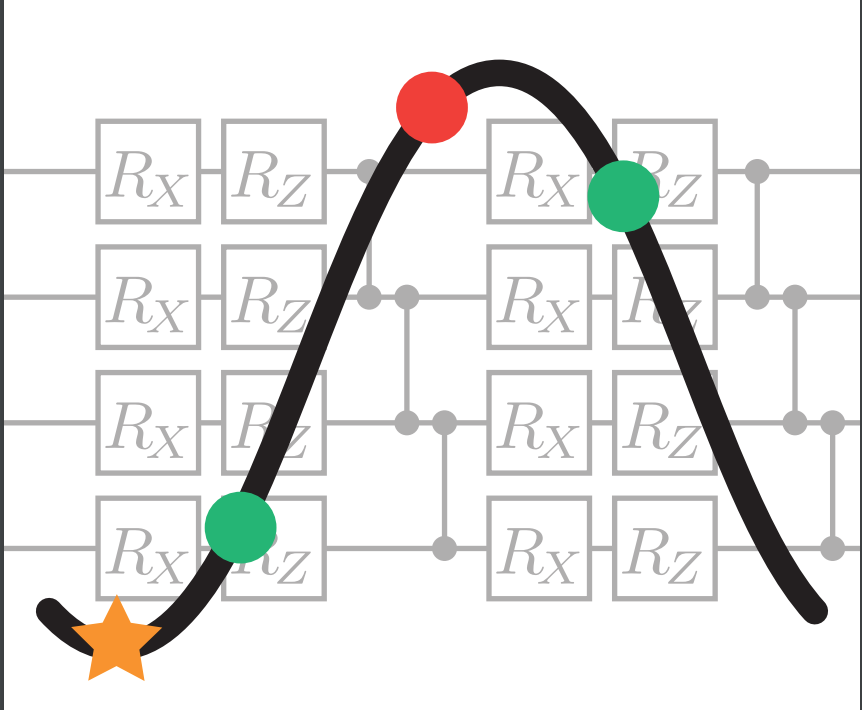
\includegraphics[width=0.4\textwidth]{figures/variational.png}}
\end{figure}
\end{multicols}
\end{frame}

\begin{frame}[fragile]{Rational for Variational Quantum Circuits}

   \textbf{Rational:} Deliver variational quantum states $\rightarrow$ explore a
   large Hilbert space.

   \begin{columns}
     \column{5cm}
     \begin{equation*}
       U(\vec{\alpha}) = U_n \ldots U_2 U_1
     \end{equation*}
     %\vspace{cm}
     \begin{equation*}
       \Qcircuit @C=1em @R=.7em {
         & \multigate{1}{U_1} & \gate{U_3} & \qw \\
         & \ghost{U_1} & \multigate{2}{U_4} & \qw \\
         & \multigate{1}{U_2} & \ghost{U_4} & \qw \\
         & \ghost{U_2} & \ghost{U_4} & \qw \\
         }
     \end{equation*}
     \column{5.5cm}
     \begin{figure}
       Near optimal solution
       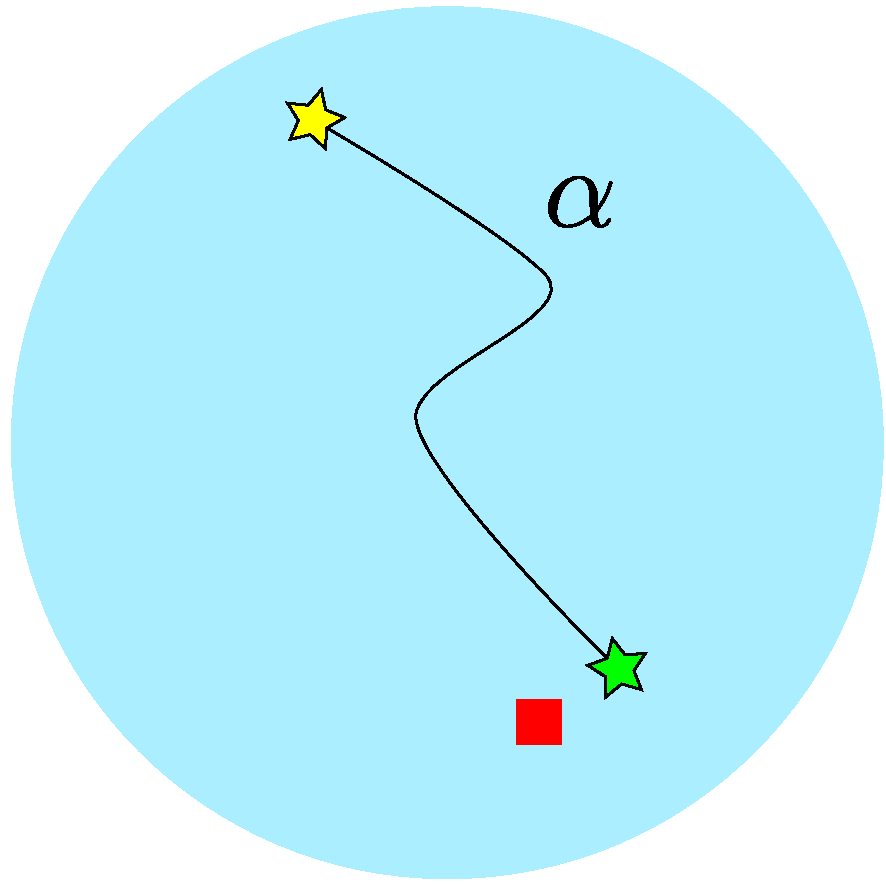
\includegraphics[scale=0.18]{figures/drawing.pdf}
     \end{figure}
   \end{columns}

   \pause
   \vspace{1cm}
   \textbf{Idea:} Quantum Computer is a machine that generates variational
   states.

     \textbf{$\Rightarrow$ Variational Quantum Computer}

 \end{frame}

 \begin{frame}[fragile]{Solovay-Kitaev Theorem}

   \begin{columns}
     \column{6cm}
     Let $\{U_i\}$ be a dense set of unitaries.

     Define a circuit approximation to $V$:
   \begin{equation*}
     |U_k \ldots U_2 U _1 - V| < \delta
   \end{equation*}
   Scaling to best approximation
   \begin{equation*}
     k \sim \mathcal{O}\left(\log^c \frac{1}{\delta} \right)
   \end{equation*}
   where $c < 4$.
   \column{5cm}
   \begin{figure}
     {\color{red} Optimal solution}
     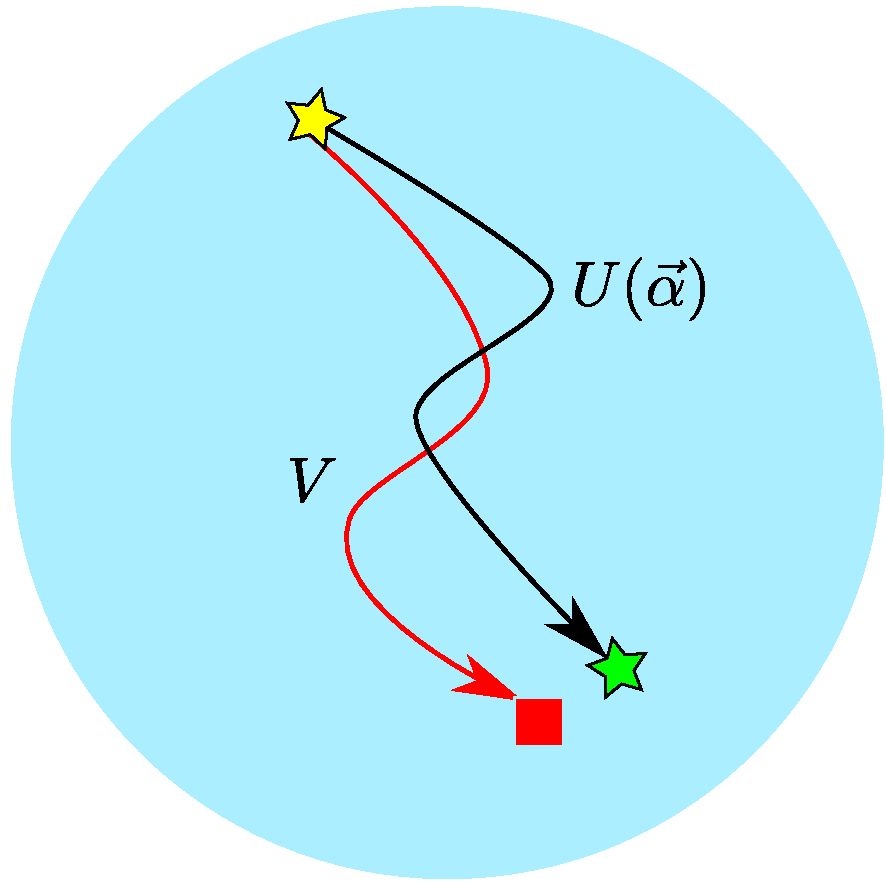
\includegraphics[scale=0.22]{figures/drawing2.pdf}
   \end{figure}
   \end{columns}

   \vspace{0.5cm}
   $\Rightarrow$ The approximation is {\color{blue}efficient} and requires a {\color{magenta}finite number of gates}.

 \end{frame}

\section{Quantum software challenges}

\begin{frame}{Software and Quantum Computing}
   \begin{figure}
     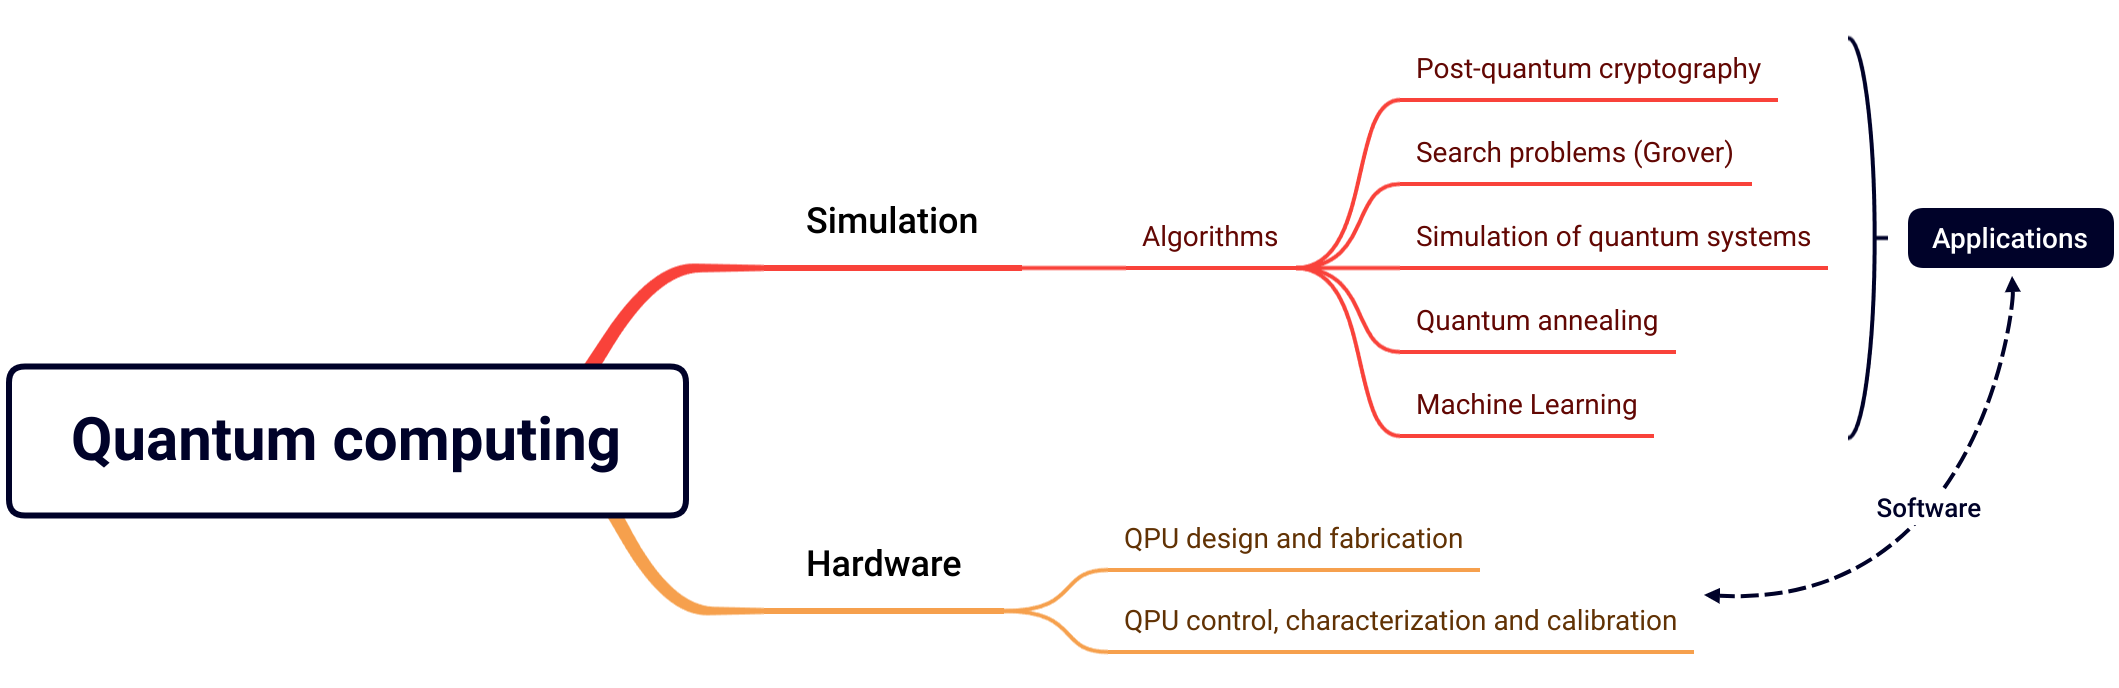
\includegraphics[height=4.7cm]{figures/q1.png}
   \end{figure}
 \end{frame}

\begin{frame}{Full-stack deployment process}
   \begin{columns}
     \column{9.2cm}
     \begin{figure}
       \only<1>{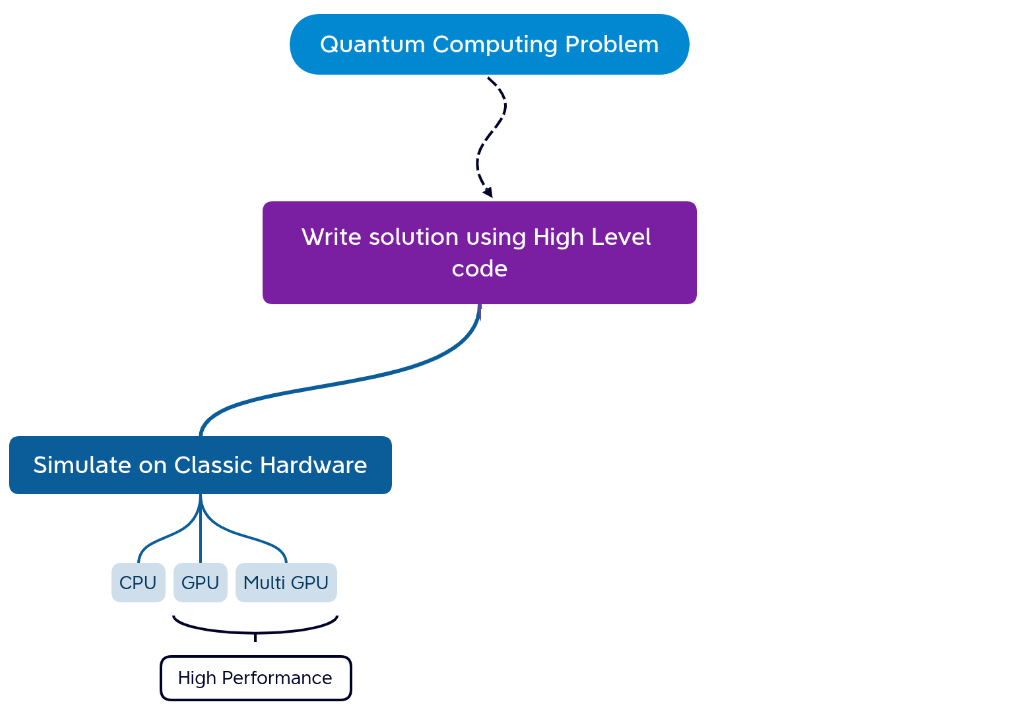
\includegraphics[height=6.5cm]{figures/challenge0.png}}
       \only<2>{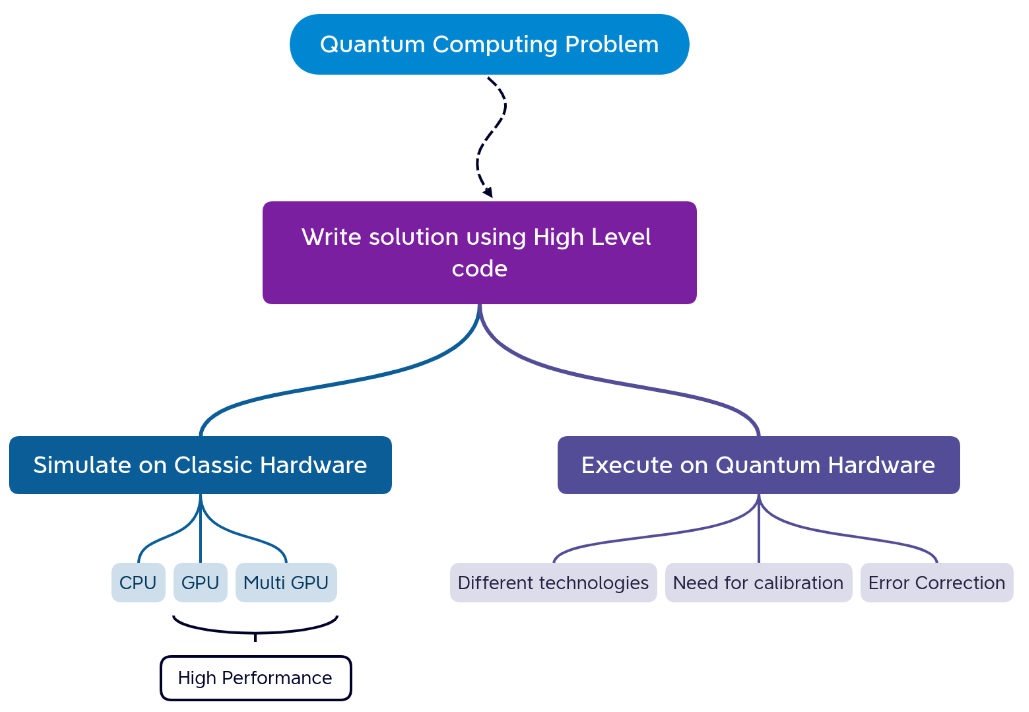
\includegraphics[height=6.5cm]{figures/challenge.png}}
     \end{figure}
   \column{6cm}
   \begin{block}{1. Prototyping}
     \begin{itemize}
       \item High-level programming language
     \end{itemize}
     \end{block}
     \begin{exampleblock}{2. Simulation}
       \begin{itemize}
         \item Fast classical quantum simulation
       \end{itemize}
   \end{exampleblock}
   \only<2>{
   \begin{alertblock}{3. Deployment on hardware}
     \begin{itemize}
       \item Hardware optimization
     \end{itemize}
   \end{alertblock}}
   \end{columns}
 \end{frame}

\begin{frame}{Software challenges}
   Requirements for self-hosted quantum hardware:
   \begin{itemize}
   \item[1.] Access to {\color{violet} \bf interdisciplinary set of software tools} for:
   \begin{figure}
     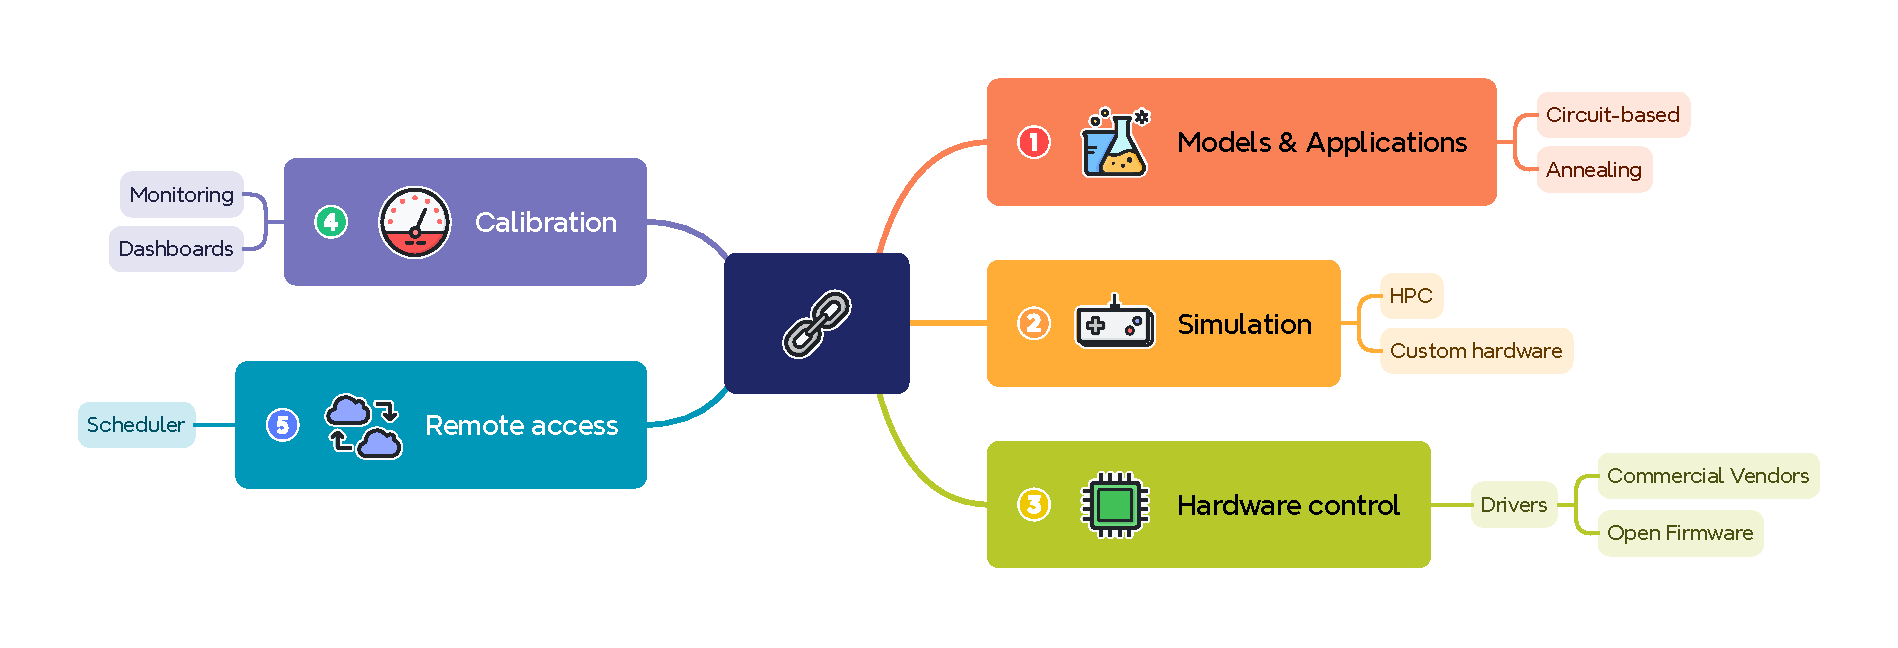
\includegraphics[width=0.95\textwidth]{figures/challenges.pdf}
   \end{figure}
     \item[2.] {\bf \color{teal} Open-source software} tools supported by benchmarks and publications.
   \end{itemize}
 \end{frame}

\section{Introducing Qibo}

\begin{frame}{The Qibo ecosystem\hfill \faBook\,\, \href{https://arxiv.org/abs/2009.01845}{arXiv:2009.01845}}

   \textbf{Qibo} is an \textbf{open-source} hybrid quantum operating system for self-hosted quantum computers.
   \begin{columns}
     \column{8cm}
     \begin{figure}
       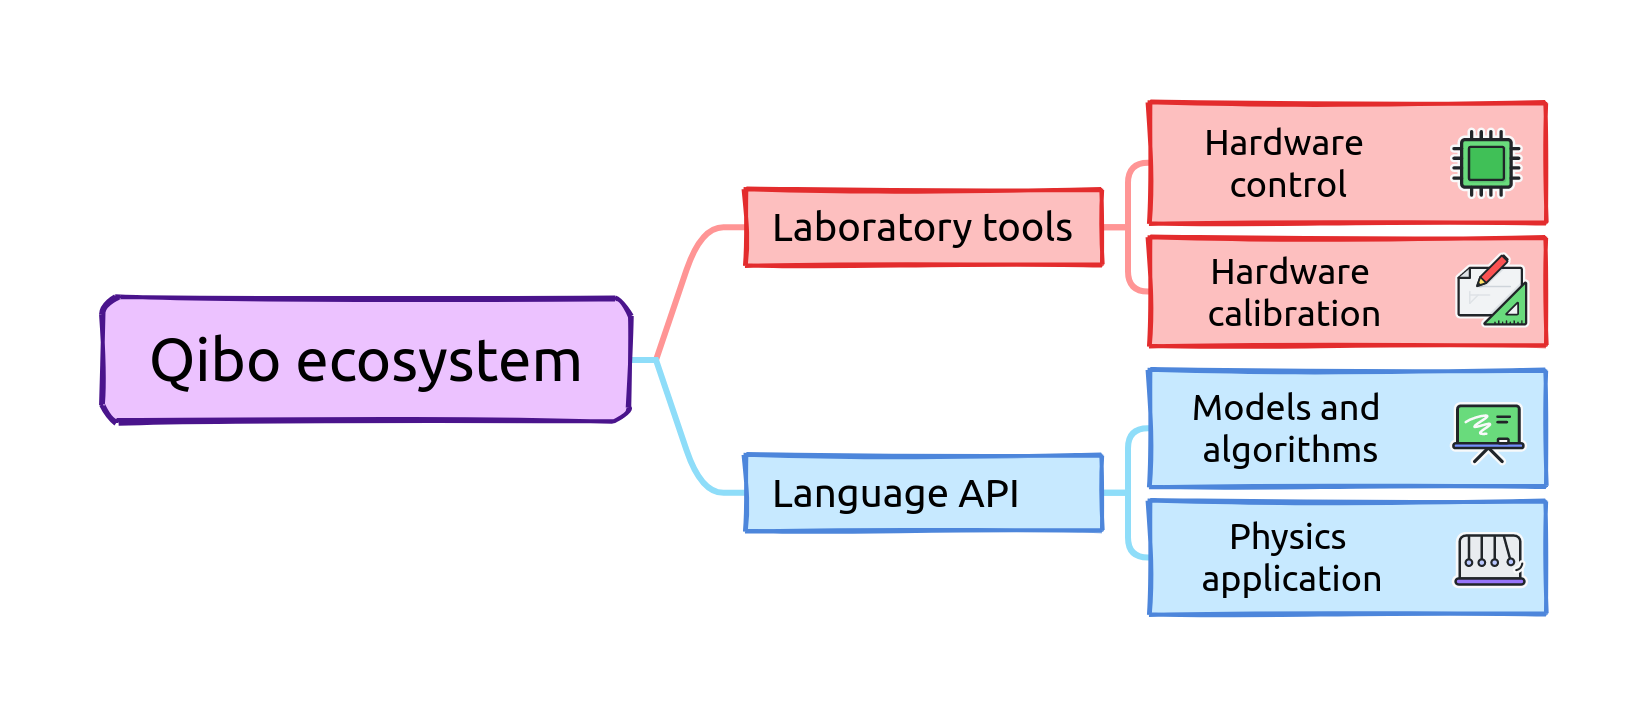
\includegraphics[width=0.7\textwidth]{figures/overview.png}
     \end{figure}
     \vspace{-0.5cm}
   \begin{enumerate}
     \item[1.] Fully open-source and community driven.
     \item[2.] Modular layout design with possibility of adding:
     \begin{itemize}[noitemsep]
       \item[-] new backends for simulation,
       \item[-] new platforms for hardware control,
       \item[-] new drivers for control electronics.
     \end{itemize}
     \item[3.] Supported by documentation and tests/CI on quantum hardware.
   \end{enumerate}

     \column{5cm}
     \begin{figure}
       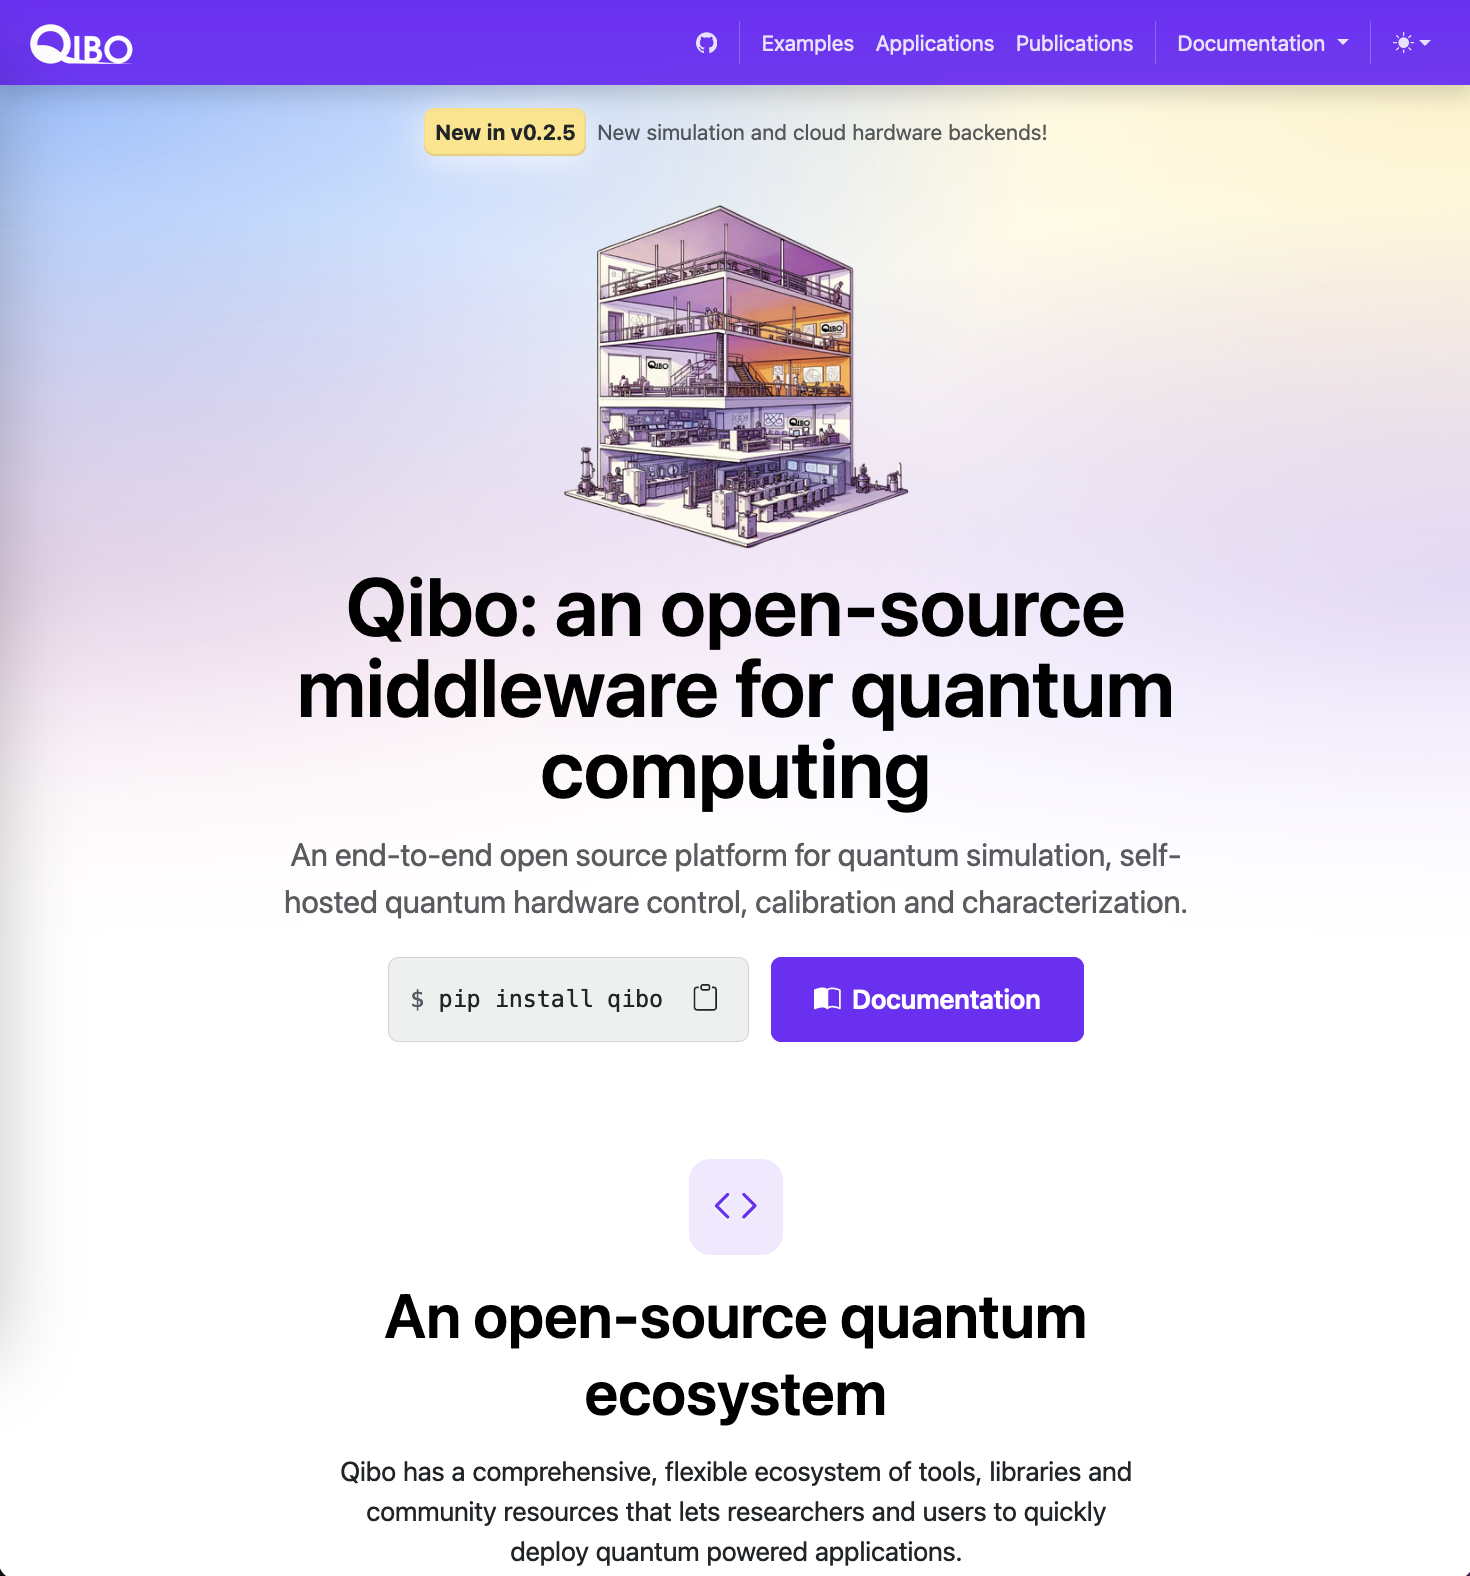
\includegraphics[width=\textwidth]{figures/docs.png}
       {\color{blue}\url{https://qibo.science}}
     \end{figure}
   \end{columns}
\end{frame}

 \begin{frame}{Qibo's macrostructure\hfill \faBook\,\, \href{https://arxiv.org/abs/2009.01845}{arXiv:2009.01845}}
   \vspace{-0.27cm}
   \begin{figure}
     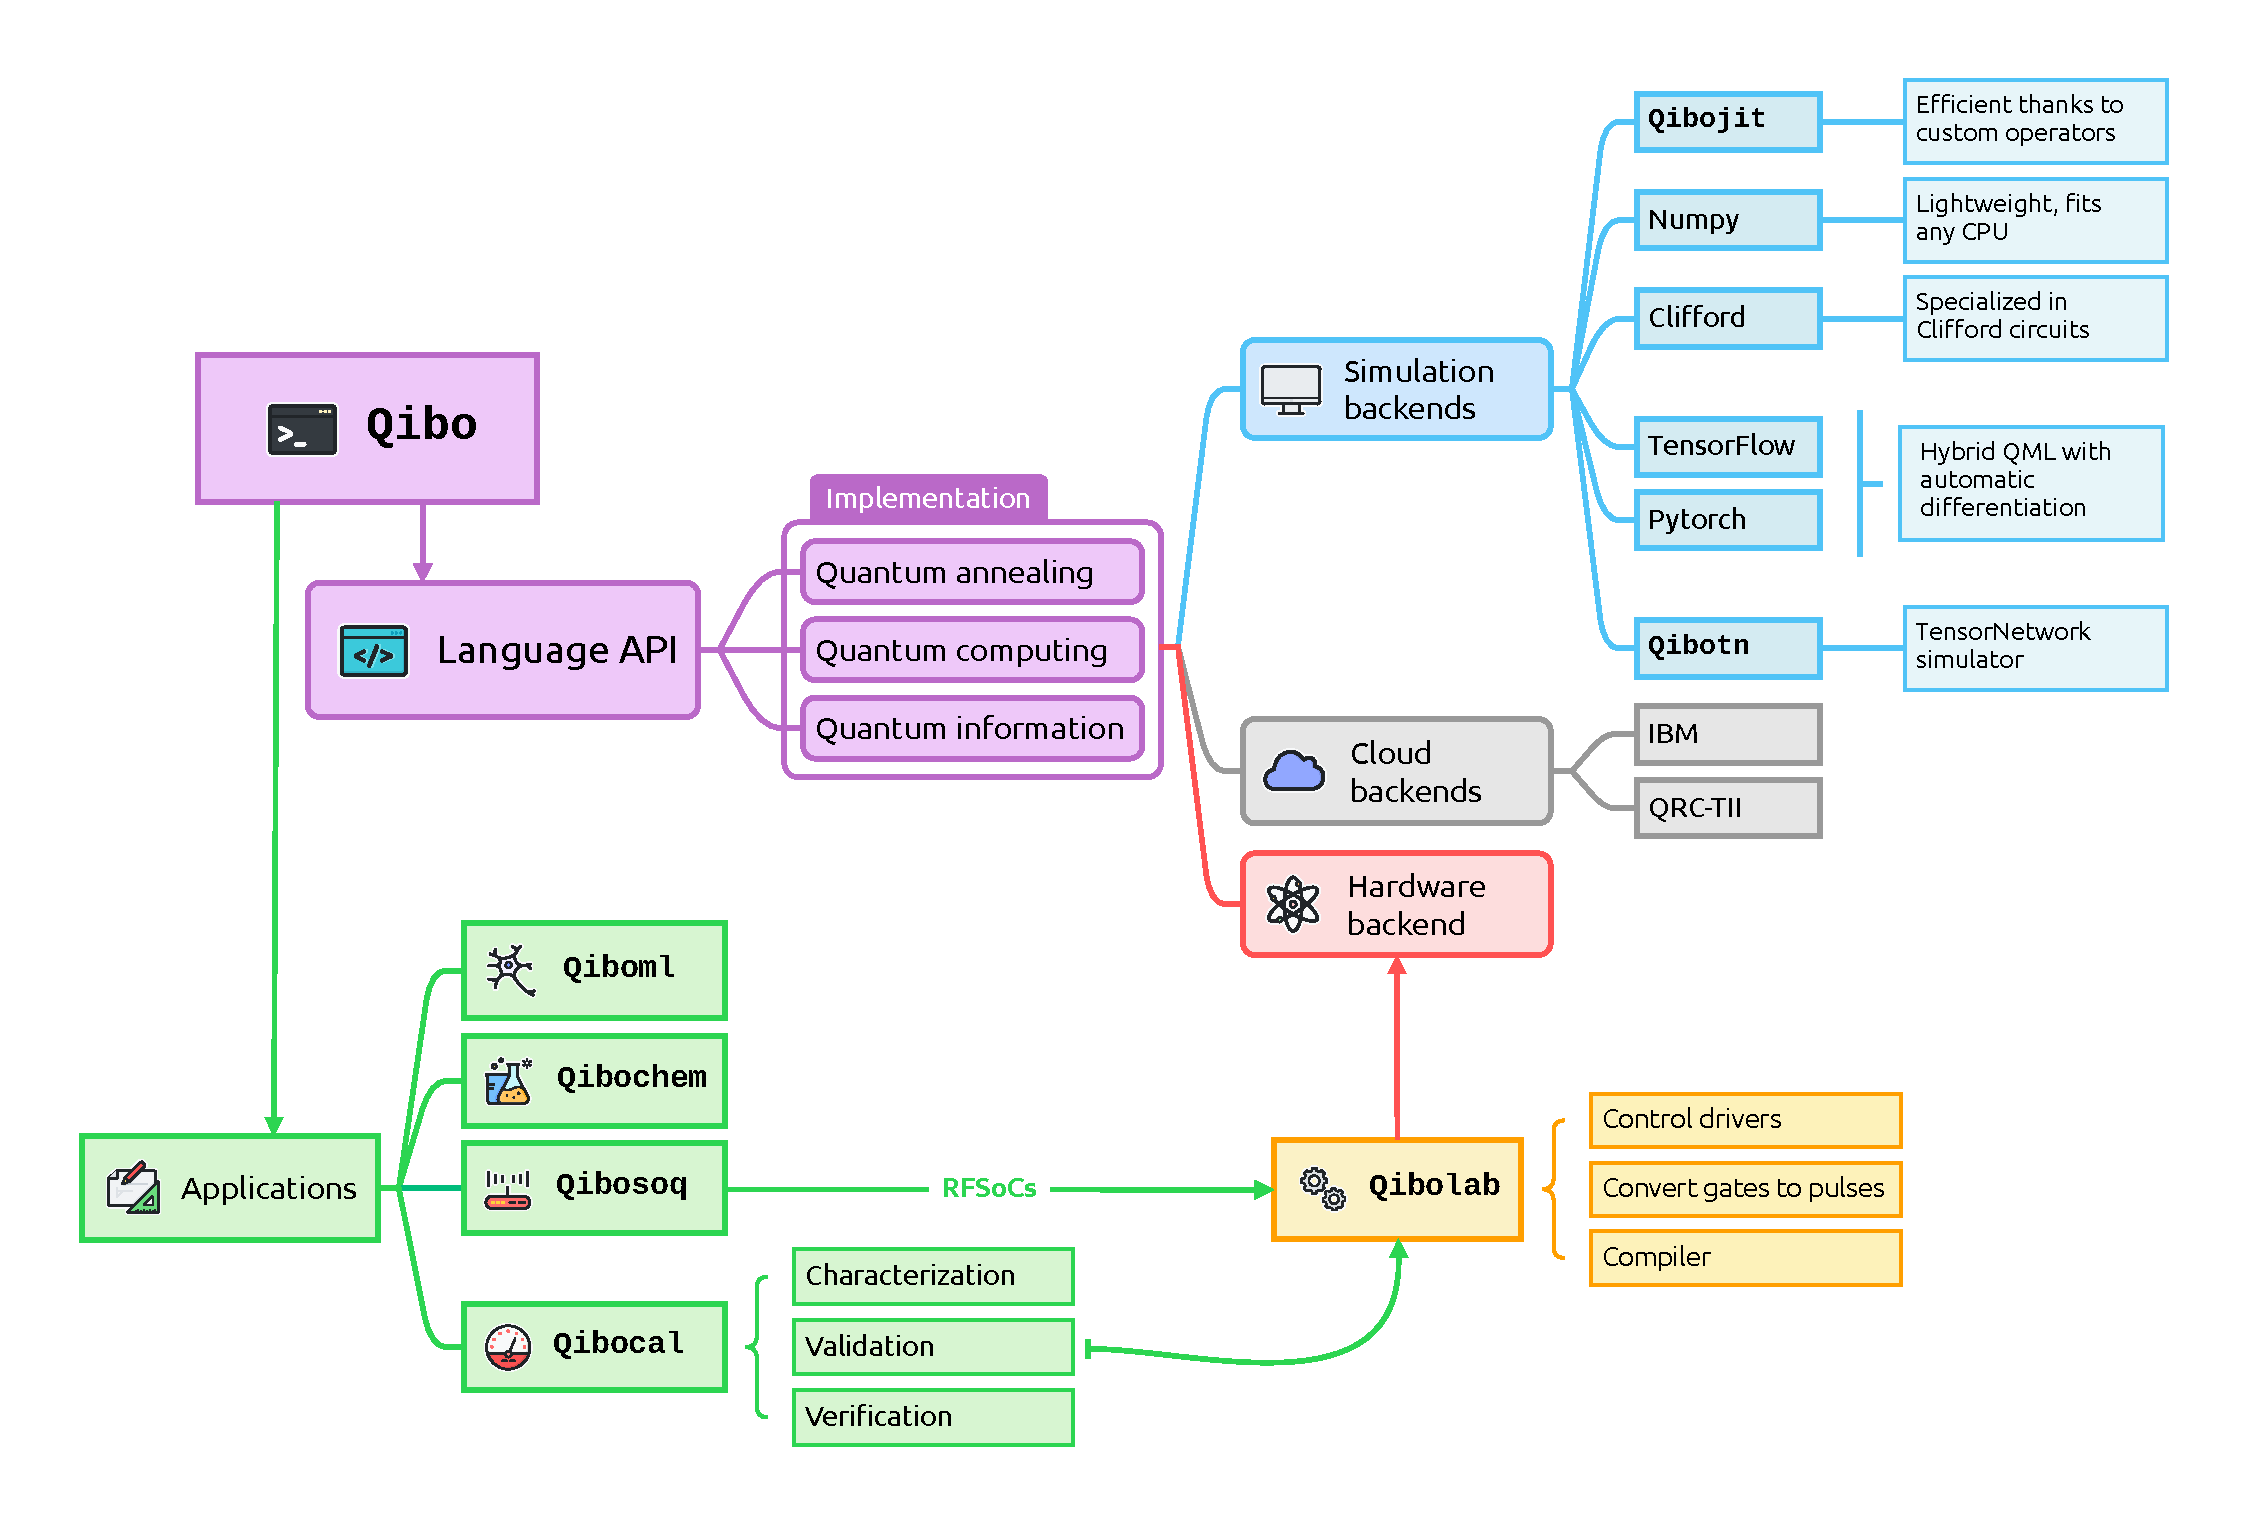
\includegraphics[height=8.3cm]{figures/qibo_ecosystem.pdf}
   \end{figure}
   \vspace{-1.3cm}
   \hfill{\footnotesize \color{blue}\url{https://qibo.science}}
 \end{frame}

 \begin{frame}{Qibo Contributors (March 2024)}
   \begin{figure}
       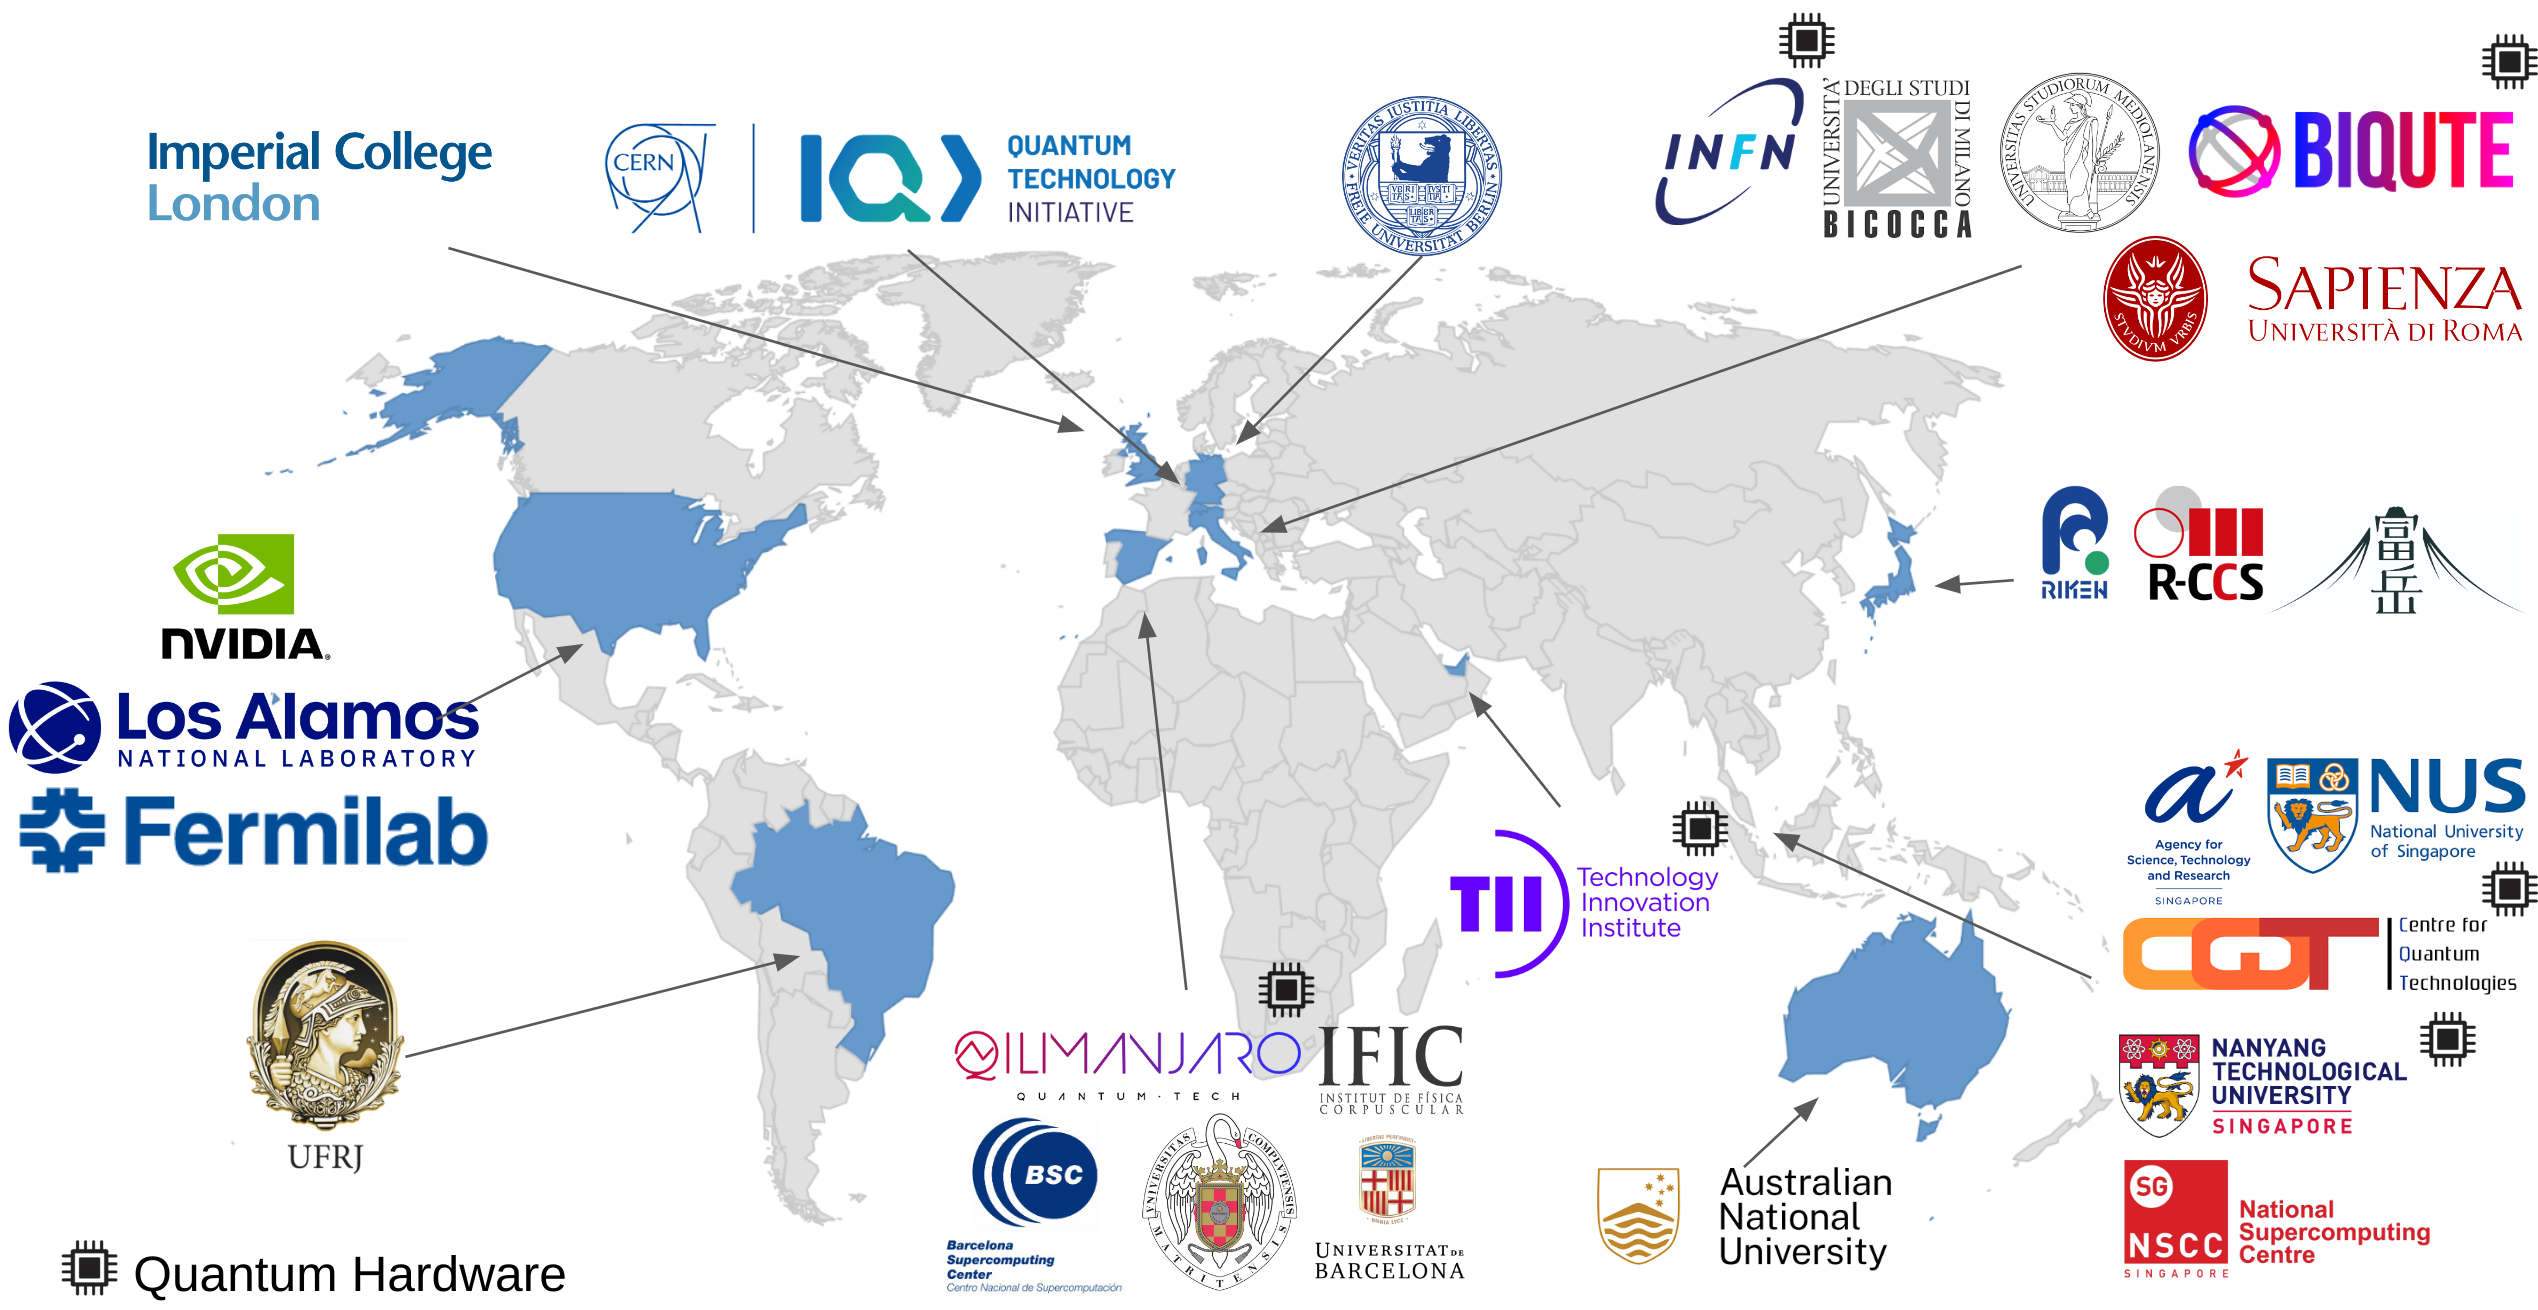
\includegraphics[height=7cm]{figures/qibocoll.png}
   \end{figure}
 \end{frame}

\section{Quantum Simulation}

\begin{frame}{Qibo backends}

  We provide a modular and extensible framework for quantum computing based on \textbf{backends}:
  \vspace{-0.5cm}
  \begin{figure}
    \only<1>{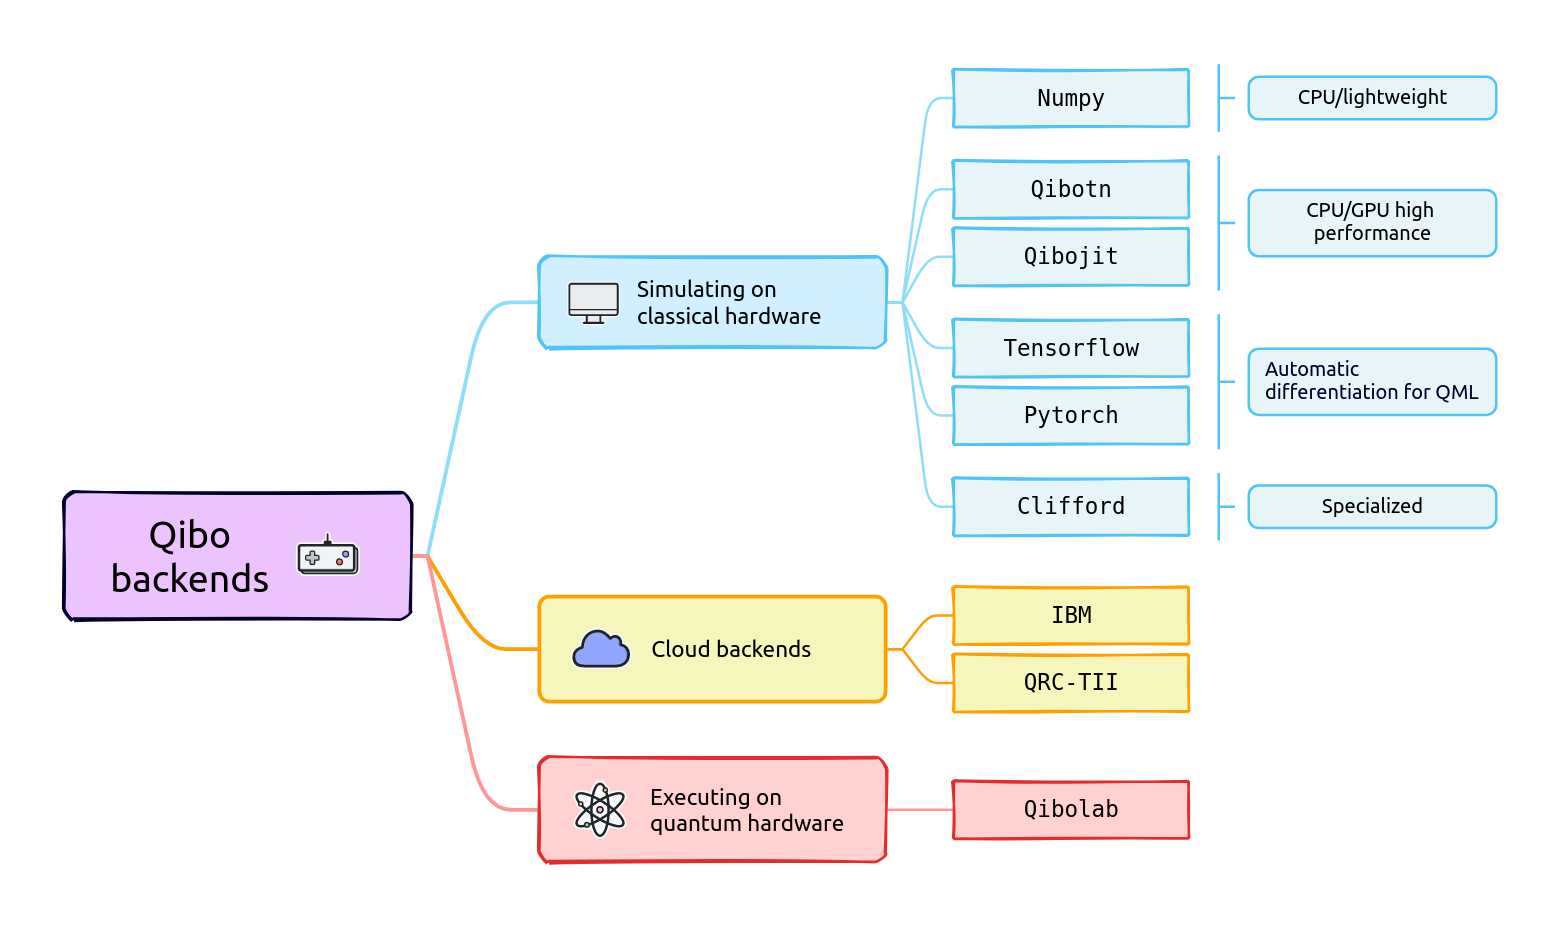
\includegraphics[height=7cm]{figures/backends.png}}
    \only<2>{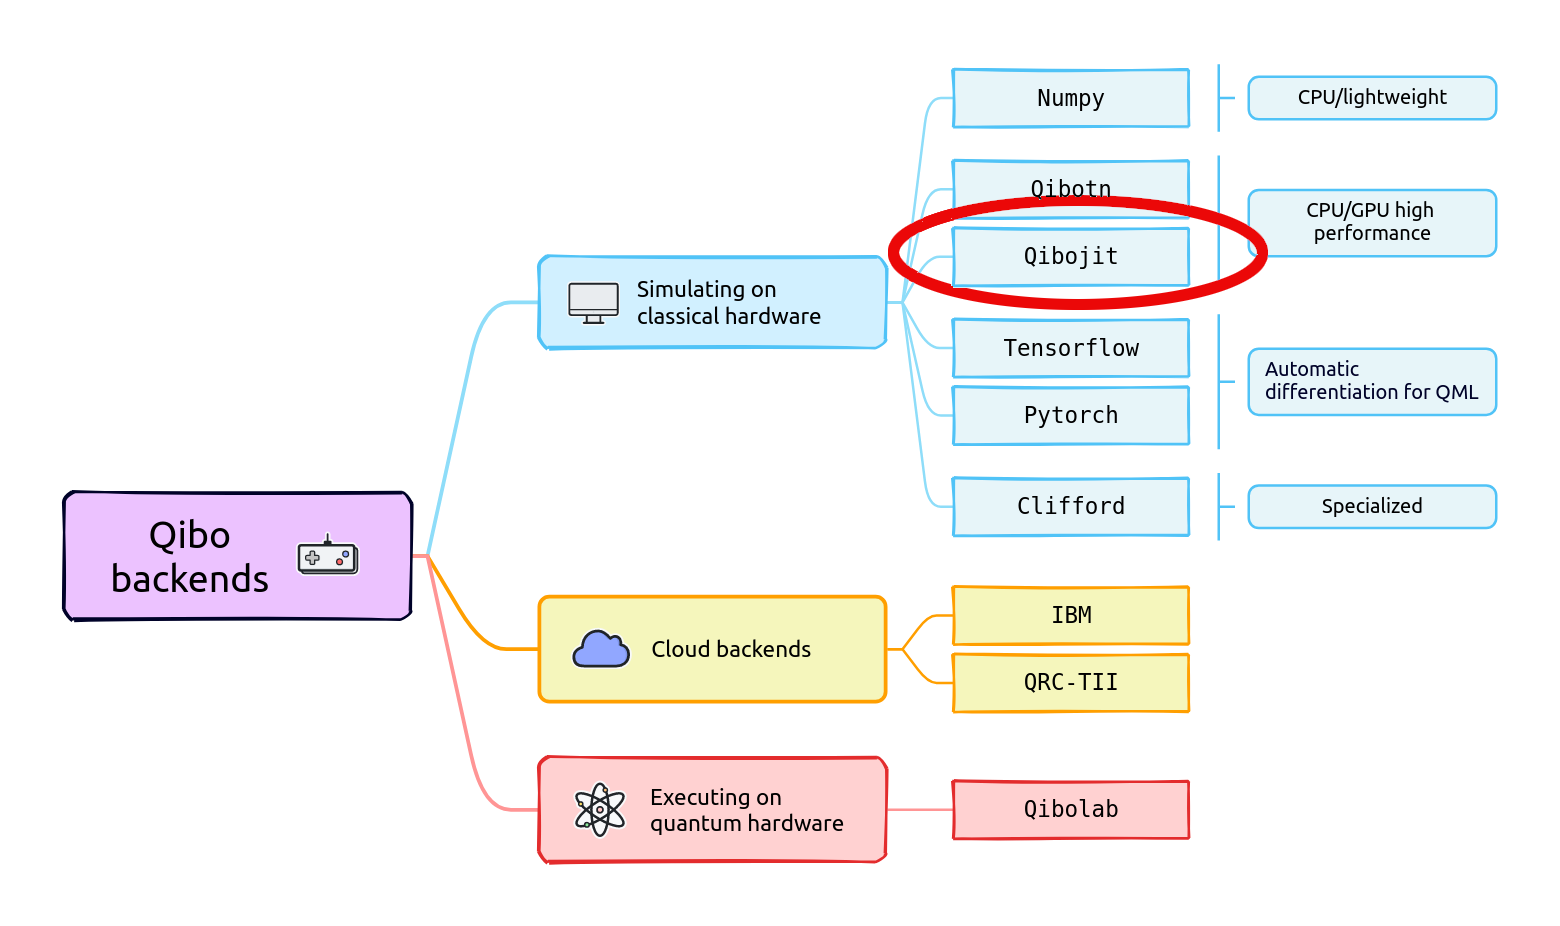
\includegraphics[height=7cm]{figures/backends2.png}}
  \end{figure}

\end{frame}

\begin{frame}{Classical quantum simulation benchmarks \hfill \faBook\,\, \href{https://arxiv.org/abs/2203.08826}{arXiv:2203.08826}}

   State vector simulation solves:
   \begin{equation*}
     \psi' (\sigma_1,\ldots,\sigma_n) = \sum_{\boldsymbol \tau'} G({\boldsymbol \tau},{\boldsymbol \tau}') \psi(\sigma_1,\ldots,{\boldsymbol \tau}',\ldots,\sigma_n)
   \end{equation*}
   The number of operations scales {\color{magenta} exponentially} with the number of qubits.

   \textbf{Qibo} uses just-in-time technology and hardware acceleration:
   \vspace{-0.35cm}
   \begin{figure}
     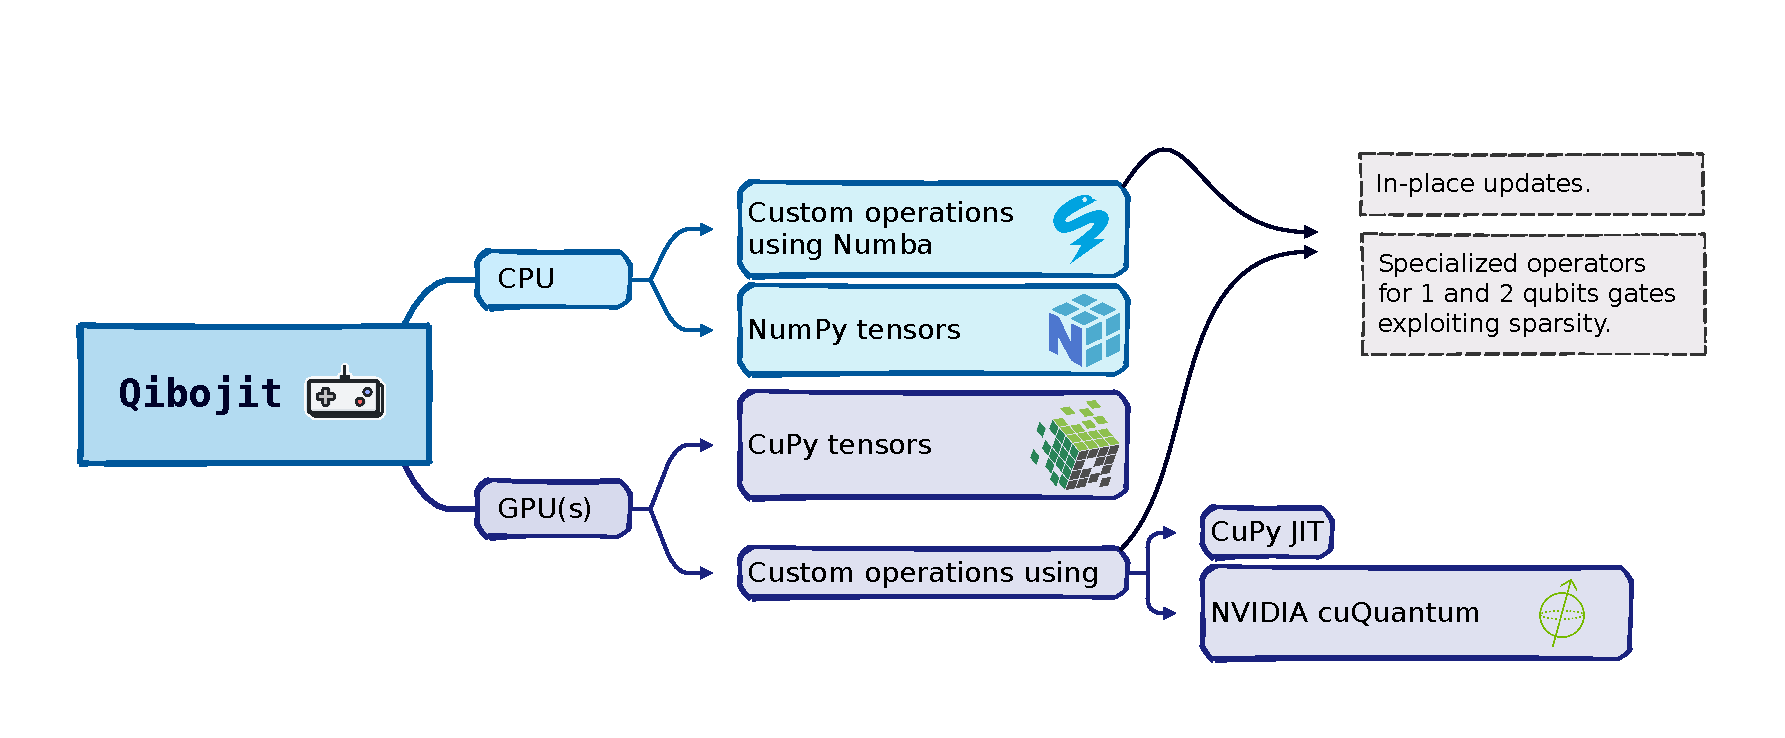
\includegraphics[height=5cm]{figures/qibojit.pdf}
   \end{figure}

 \end{frame}

 \begin{frame}{Classical quantum simulation benchmarks \hfill \faBook\,\, \href{https://arxiv.org/abs/2203.08826}{arXiv:2203.08826}}

   \begin{columns}
     \column{7cm}

   \begin{figure}
     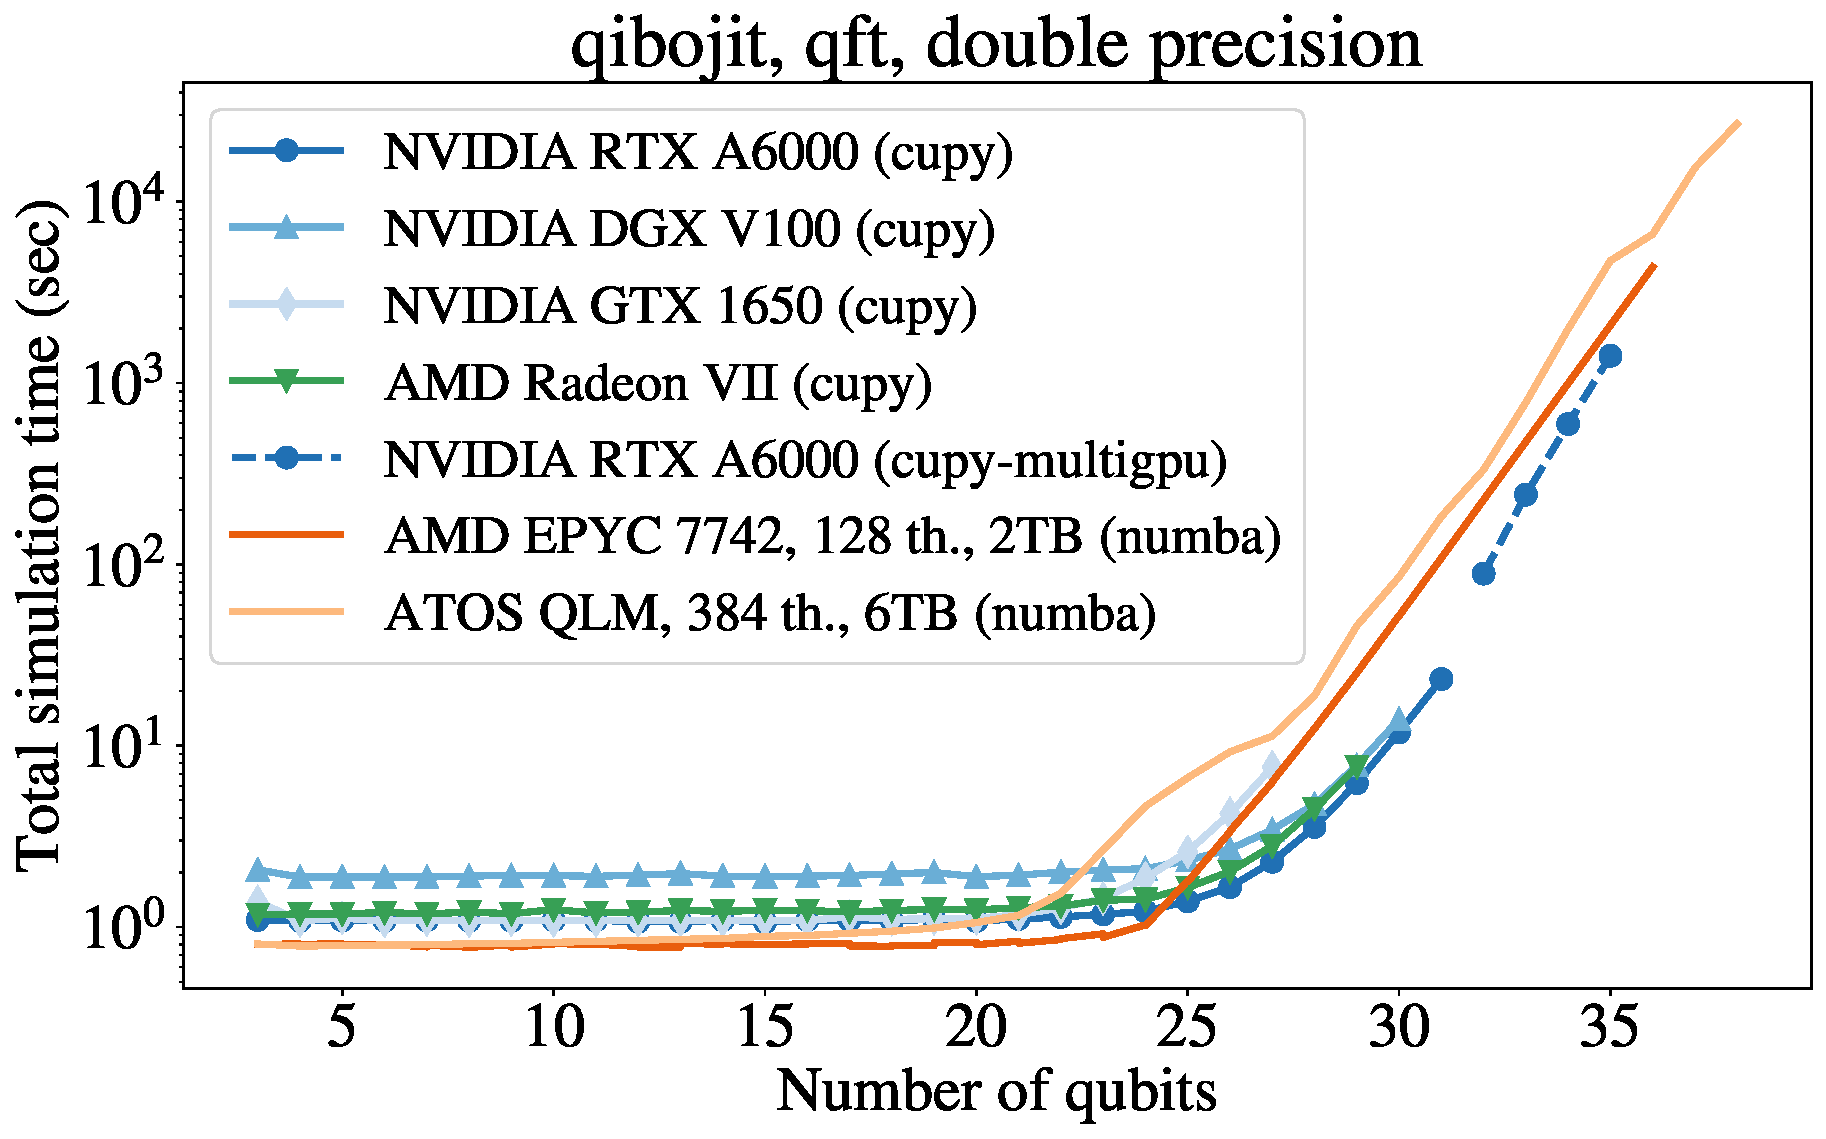
\includegraphics[width=\textwidth]{figures/devices_qft_total_simulation_time_double.pdf}
   \end{figure}

     \column{7cm}
     \begin{exampleblock}{Major features:}
       \begin{itemize}
         \item Supports CPU, GPU and multi-GPU.
         \item NVIDIA and AMD GPUs support.
         \item Reduced memory footprint.
       \end{itemize}
     \end{exampleblock}
     \begin{figure}
       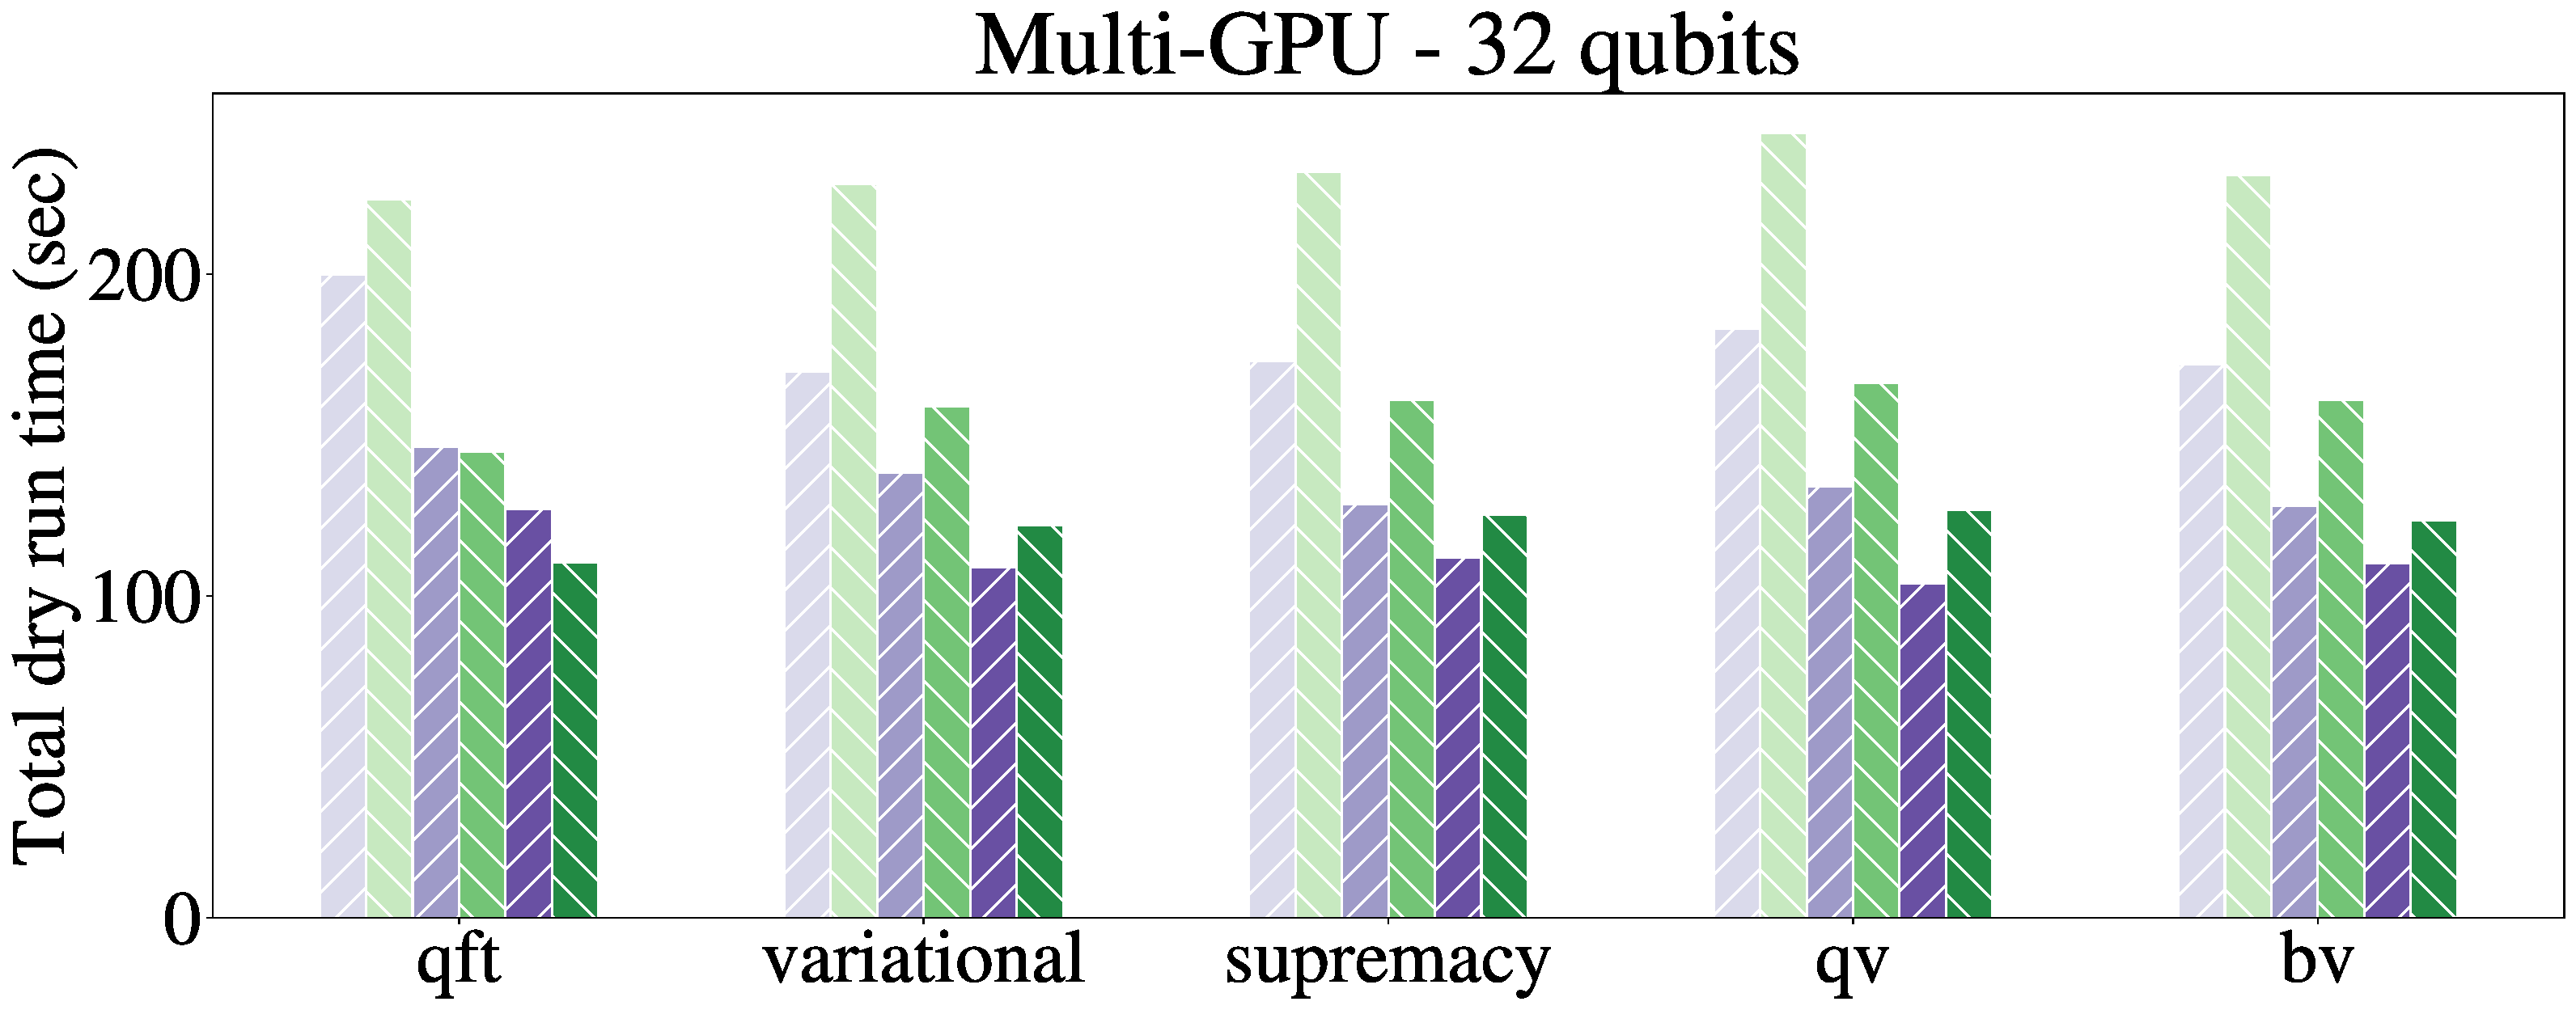
\includegraphics[width=\textwidth]{figures/multigpu_32qubits_total_dry_time_double.pdf}
     \end{figure}
   \end{columns}

   {\small {\bf Benchmark library}: \url{https://github.com/qiboteam/qibojit-benchmarks} }

 \end{frame}

 \begin{frame}{Qibo vs other libraries \hfill \faBook\,\, \href{https://arxiv.org/abs/2203.08826}{arXiv:2203.08826}}

   {\small {\bf Benchmark library}: \url{https://github.com/qiboteam/qibojit-benchmarks} }

   \begin{figure}
     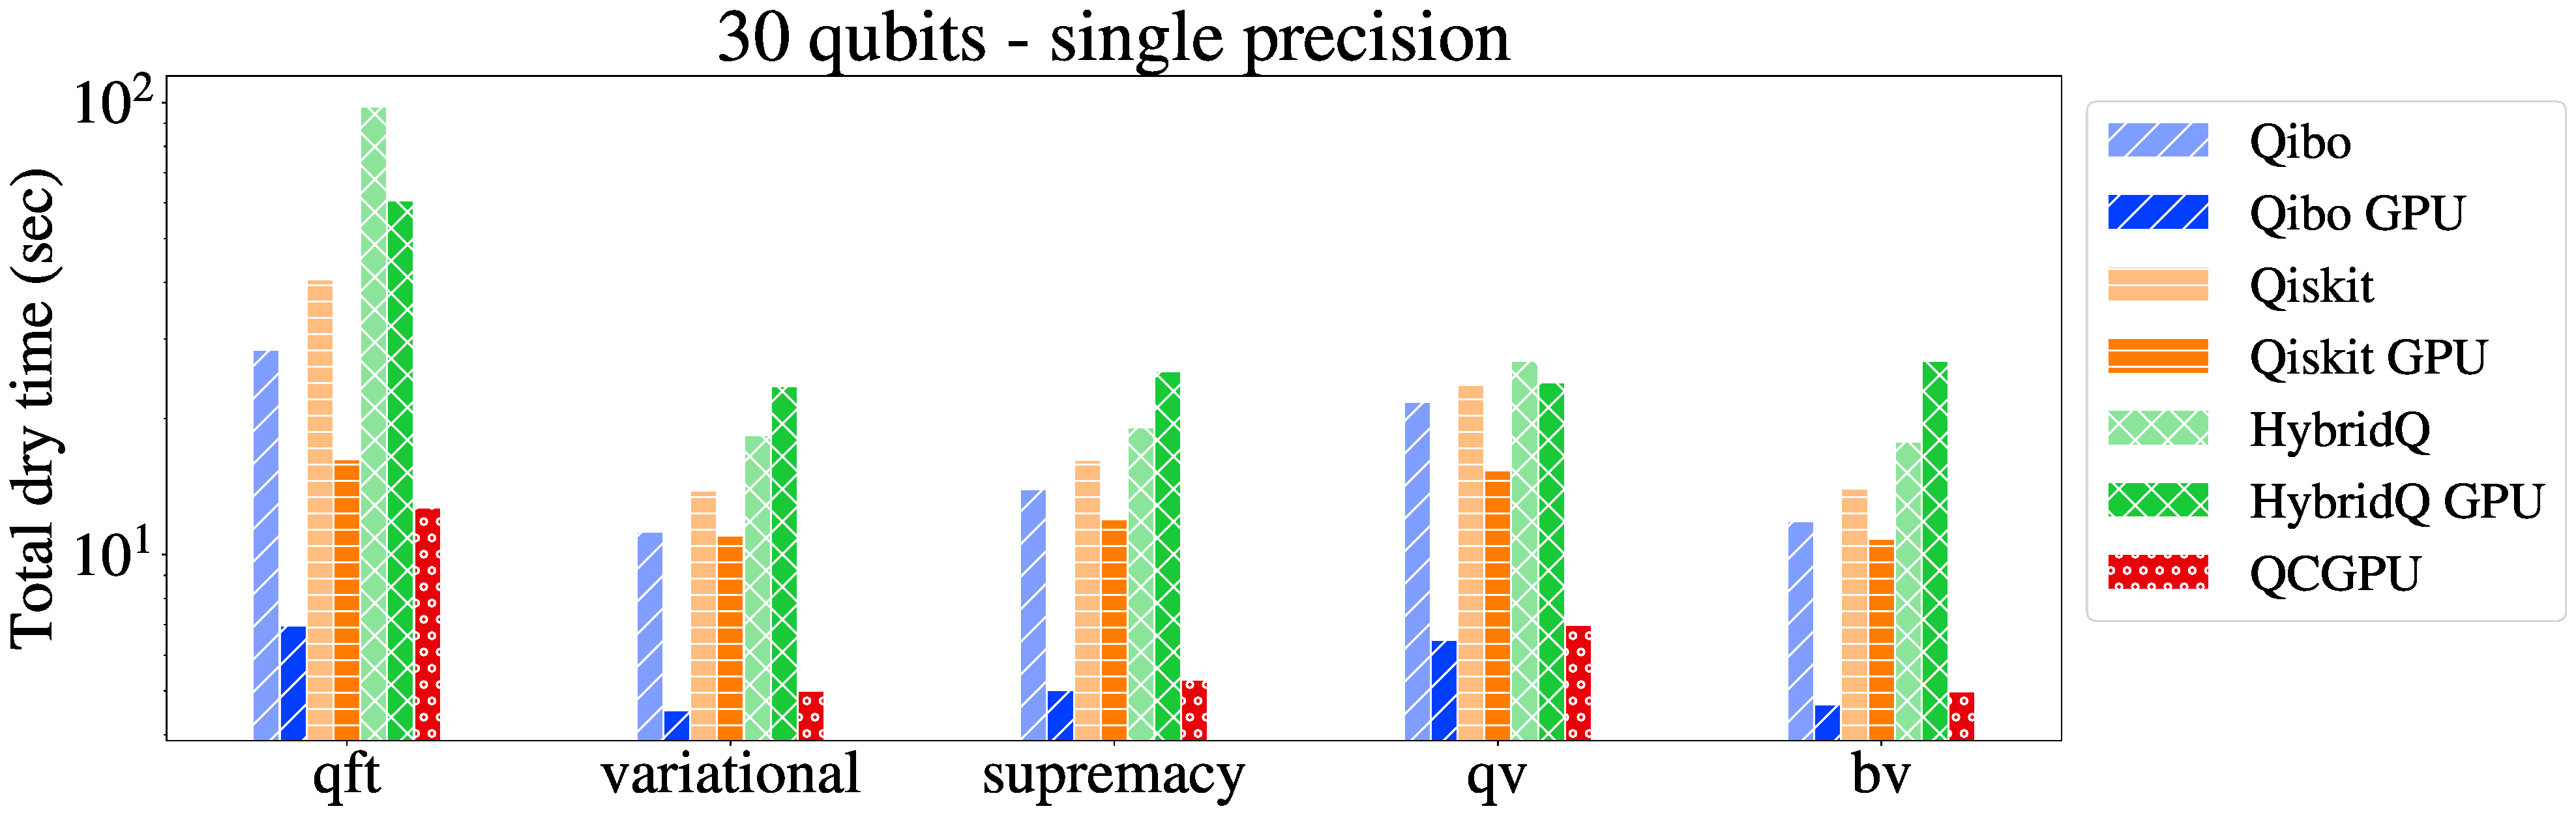
\includegraphics[scale=0.15]{figures/libraries_single_30qubits_total_dry_time.pdf}
     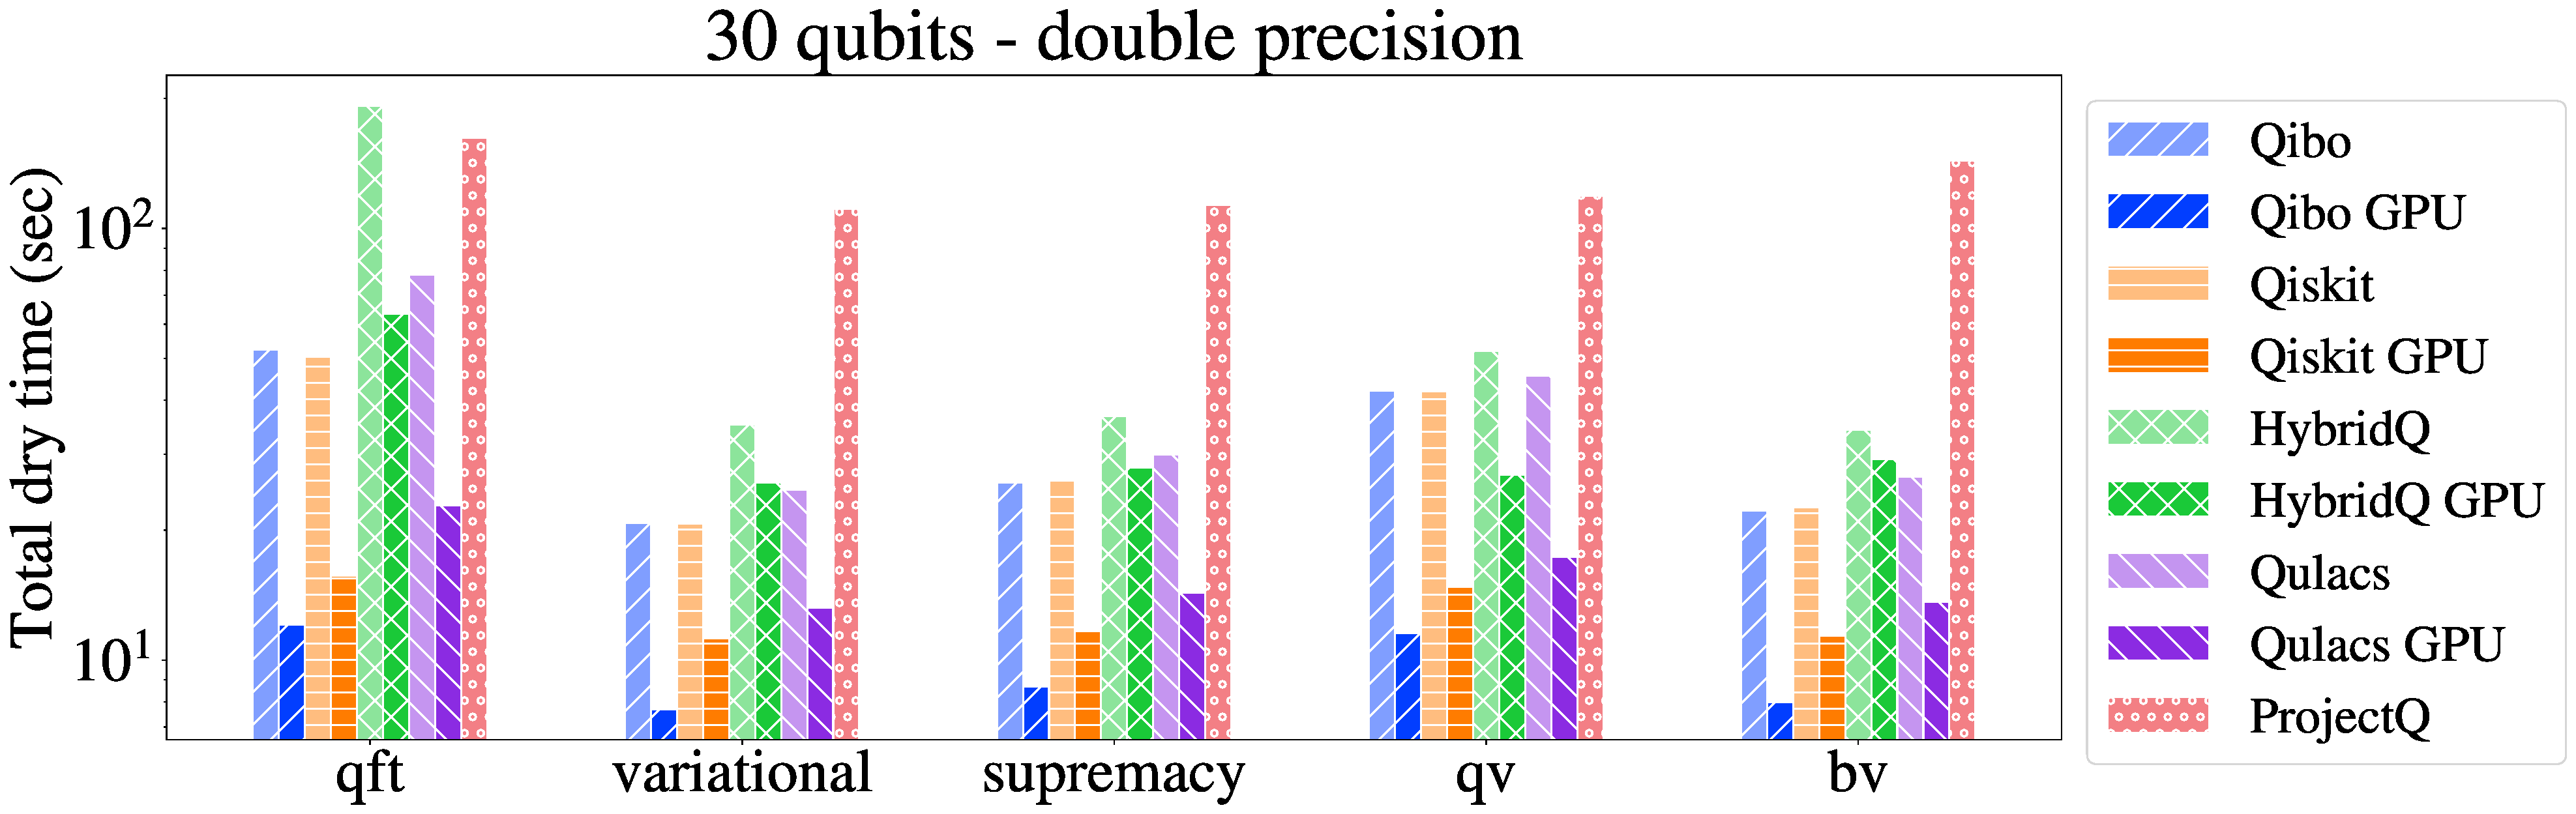
\includegraphics[scale=0.15]{figures/libraries_double_30qubits_total_dry_time.pdf}
   \end{figure}

 \end{frame}

\section{Laboratory modules}

\begin{frame}{How to control qubits?  \hfill \faBook\,\, \href{https://arxiv.org/abs/2308.06313}{arXiv:2308.06313}}
  \begin{figure}
    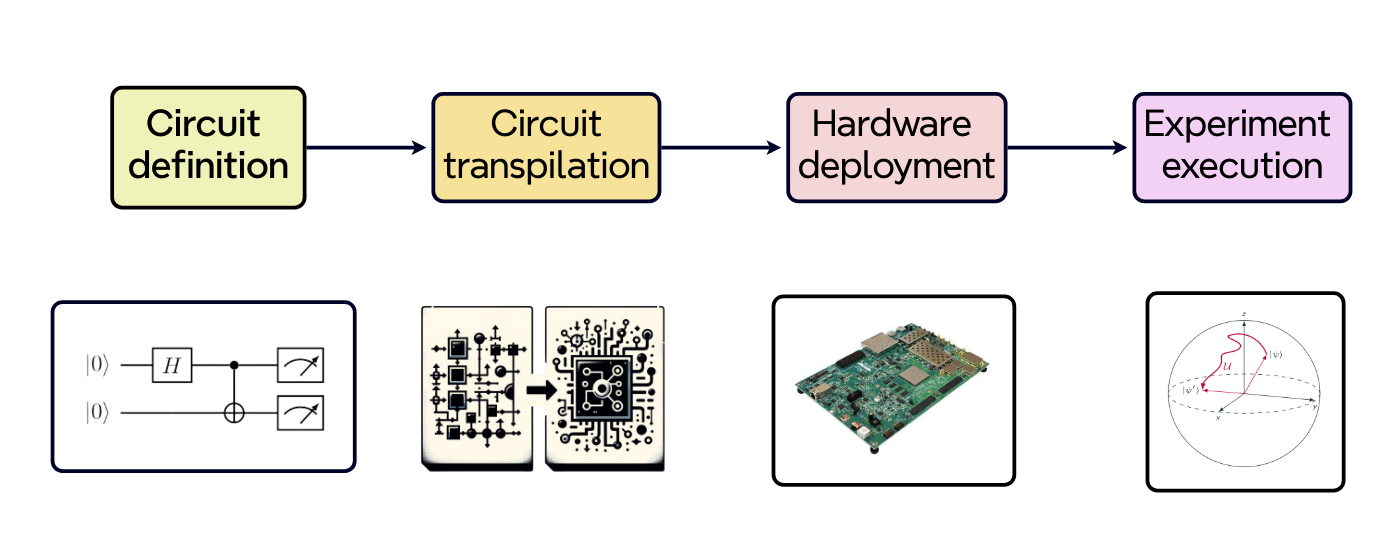
\includegraphics[width=\textwidth]{figures/algorithmdeployment.png}
  \end{figure}
\end{frame}


\begin{frame}{How to control qubits? Qibolab  \hfill \faBook\,\, \href{https://arxiv.org/abs/2308.06313}{arXiv:2308.06313}}
   \small
   \begin{columns}
     \column{6.5cm}

   \begin{figure}
     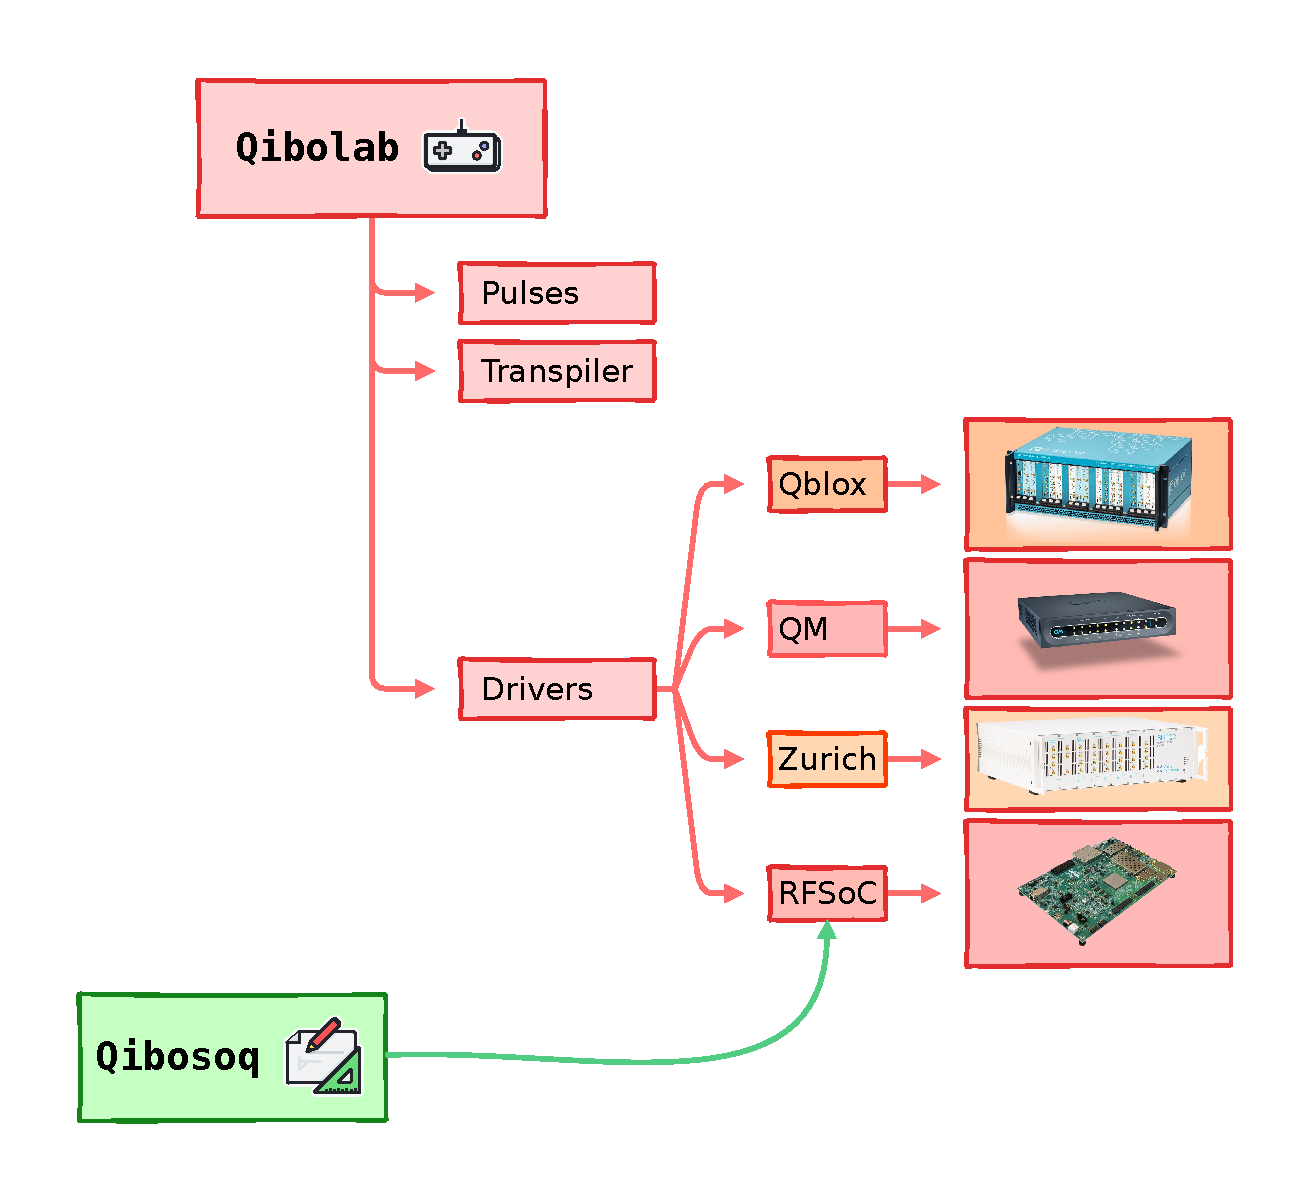
\includegraphics[width=\textwidth]{figures/instruments.pdf}
   \end{figure}

     \column{9cm}
     \begin{alertblock}{Major features:}
       \begin{itemize}
         \item Pulse and pulse sequence API.
         \item Extensible API to drivers of control instruments.
         \item Hardware sweeps for faster execution of calibration routines.
         \item Transpilers from arbitrary circuits to pulses.
         \item \texttt{C/C++} and \texttt{Rust} APIs
       \end{itemize}
     \end{alertblock}
     \begin{figure}
       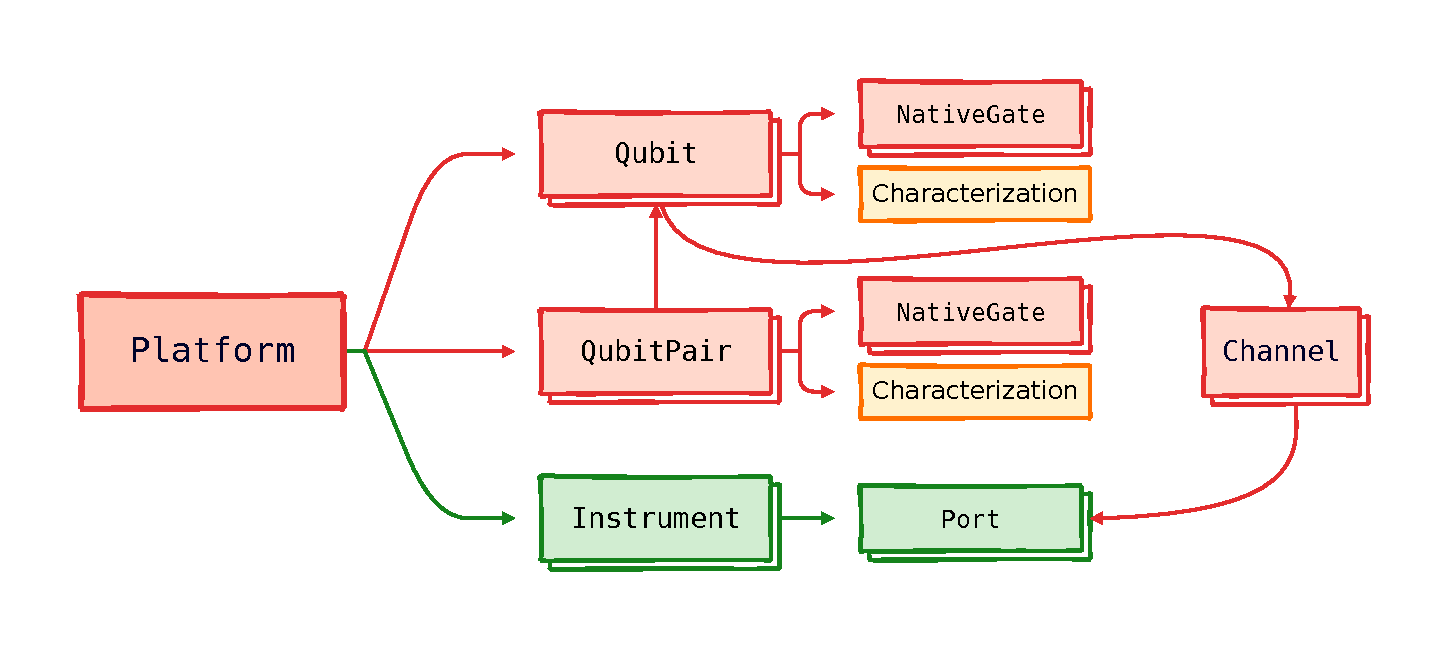
\includegraphics[width=0.9\textwidth]{figures/platform_object.pdf}
     \end{figure}
   \end{columns}

 \end{frame}


 \begin{frame}{Qubit characterization and calibration with Qibocal \hfill \faBook\,\, \href{https://arxiv.org/abs/2303.10397}{arXiv:2303.10397}}

   \begin{columns}
     \column{9cm}

   \begin{figure}
     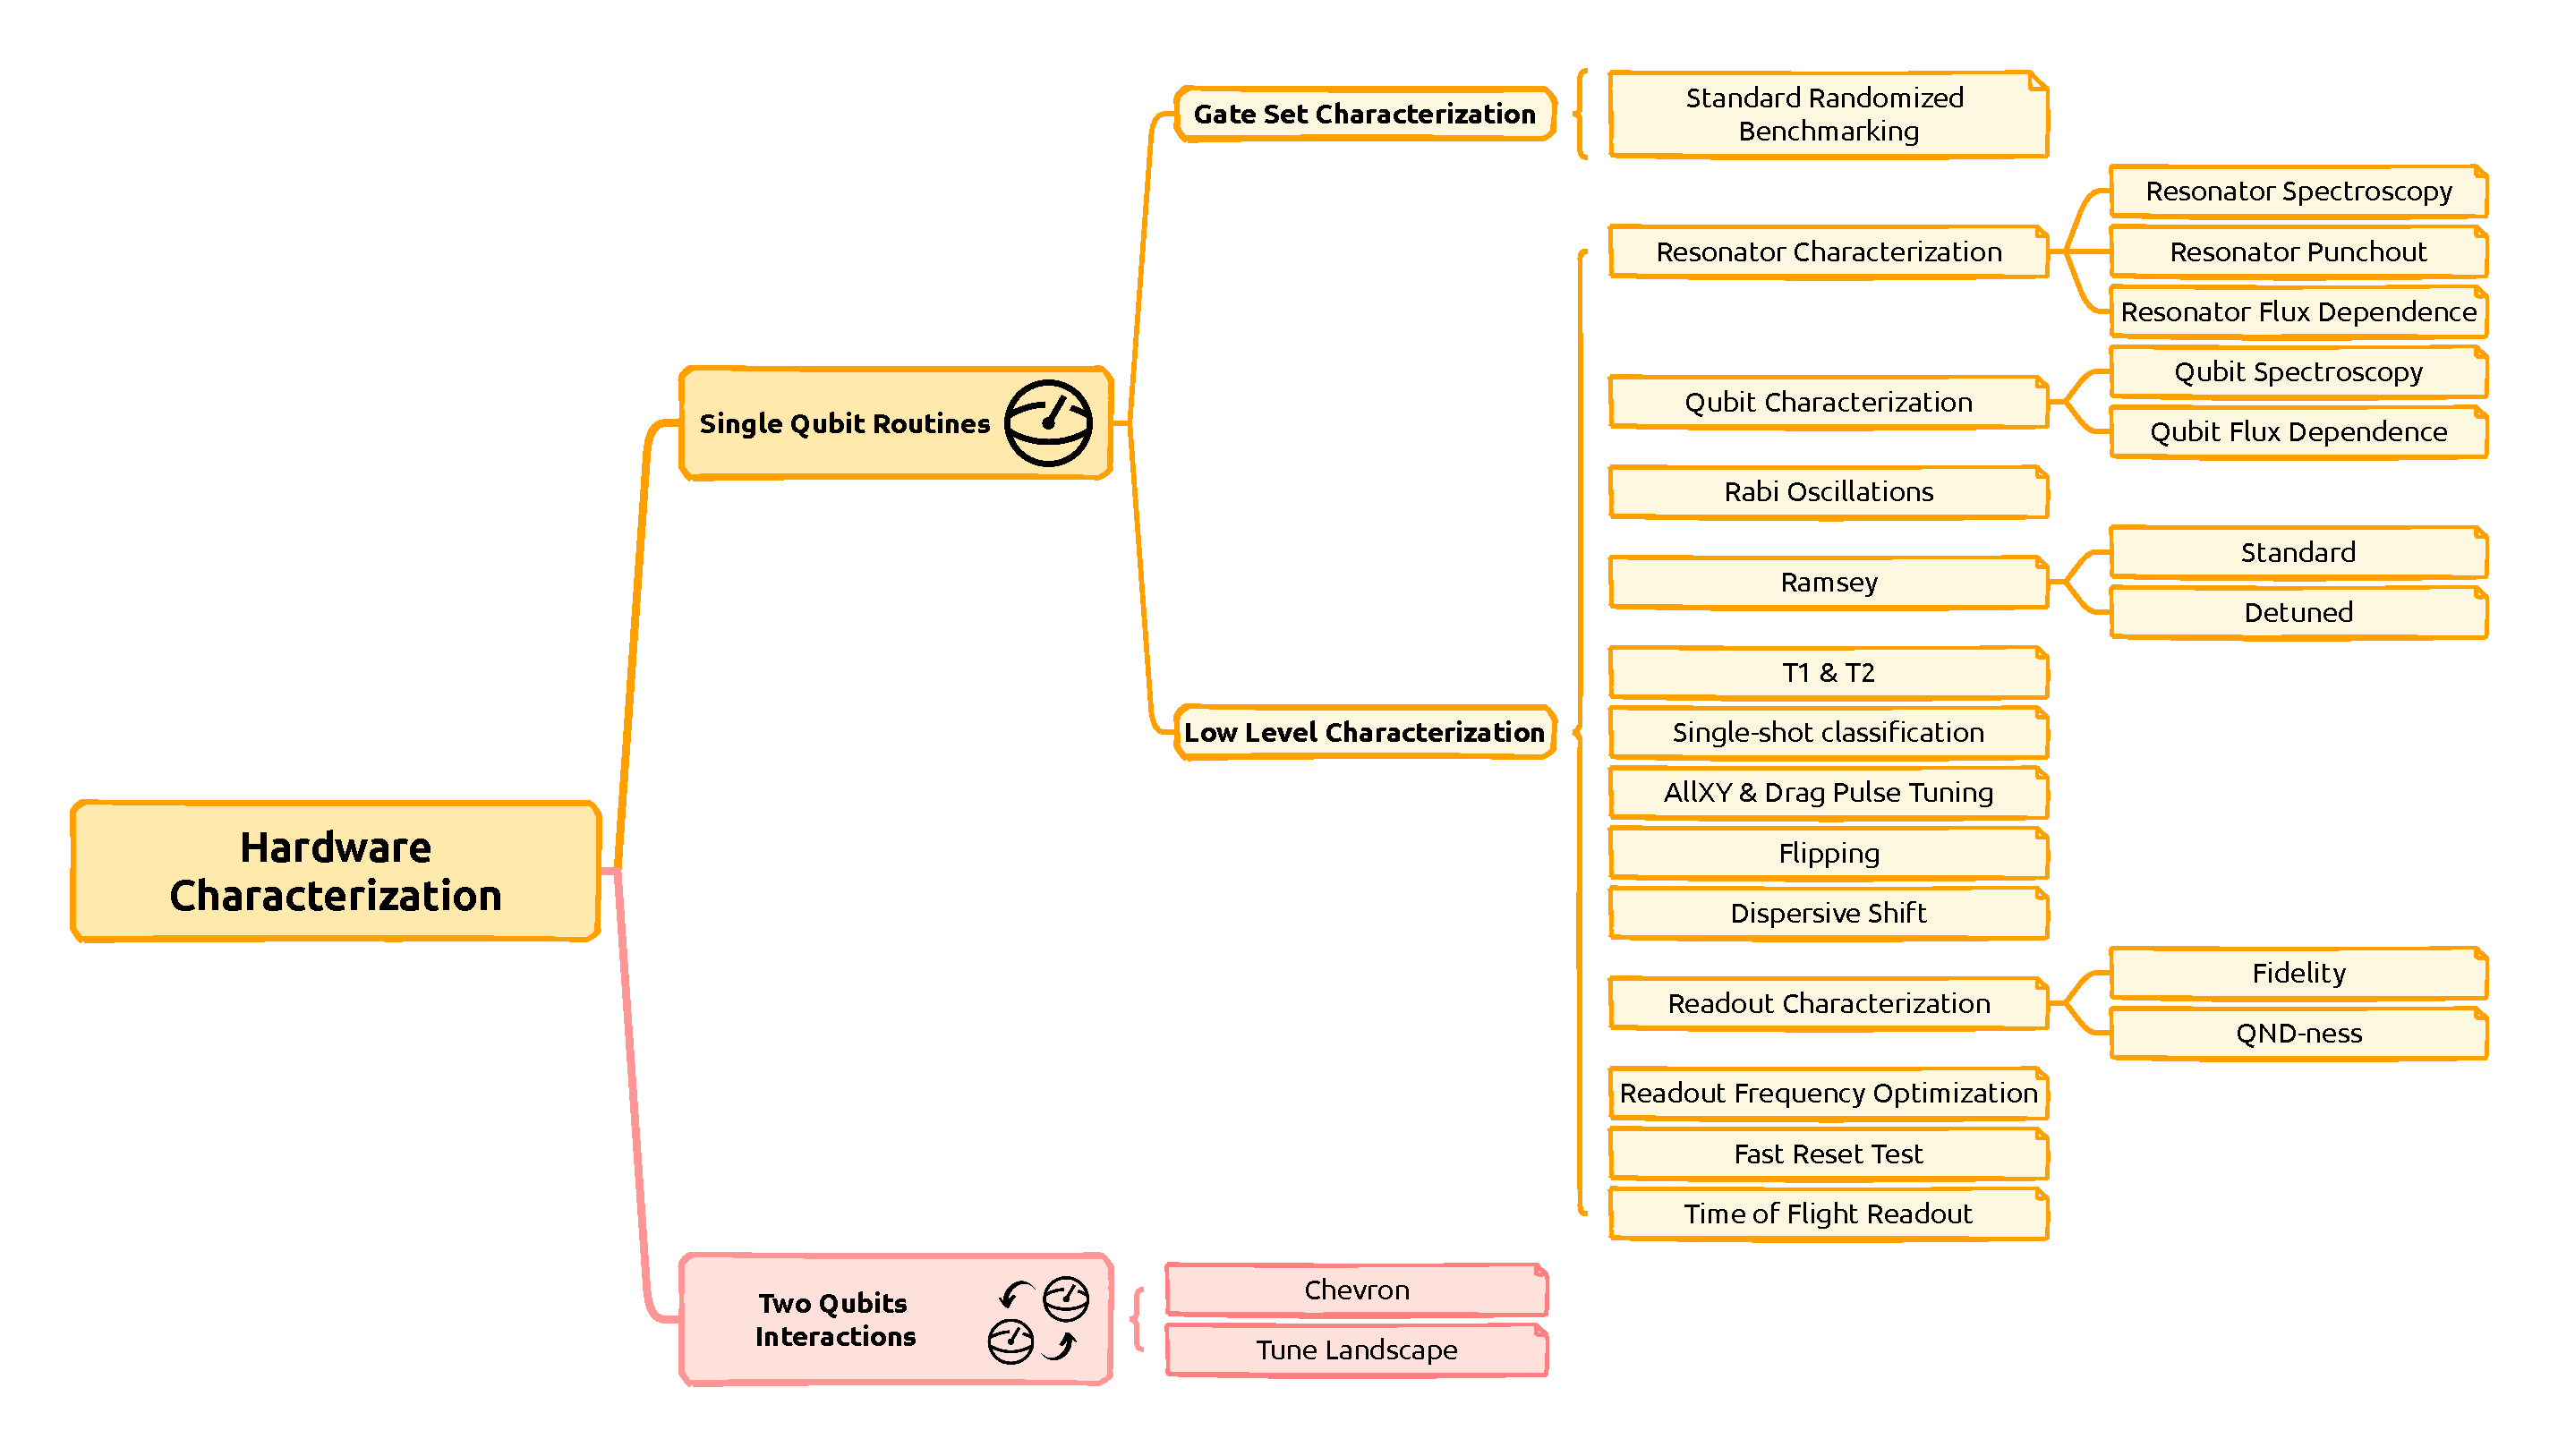
\includegraphics[width=\textwidth]{figures/qpu_characterization.pdf}
   \end{figure}

     \column{6cm}
     \begin{exampleblock}{Major features:}
       \textbf{Calibration} of single and multi-qubit platforms are possible using \textbf{Qibo}.
     \end{exampleblock}
     \begin{figure}
       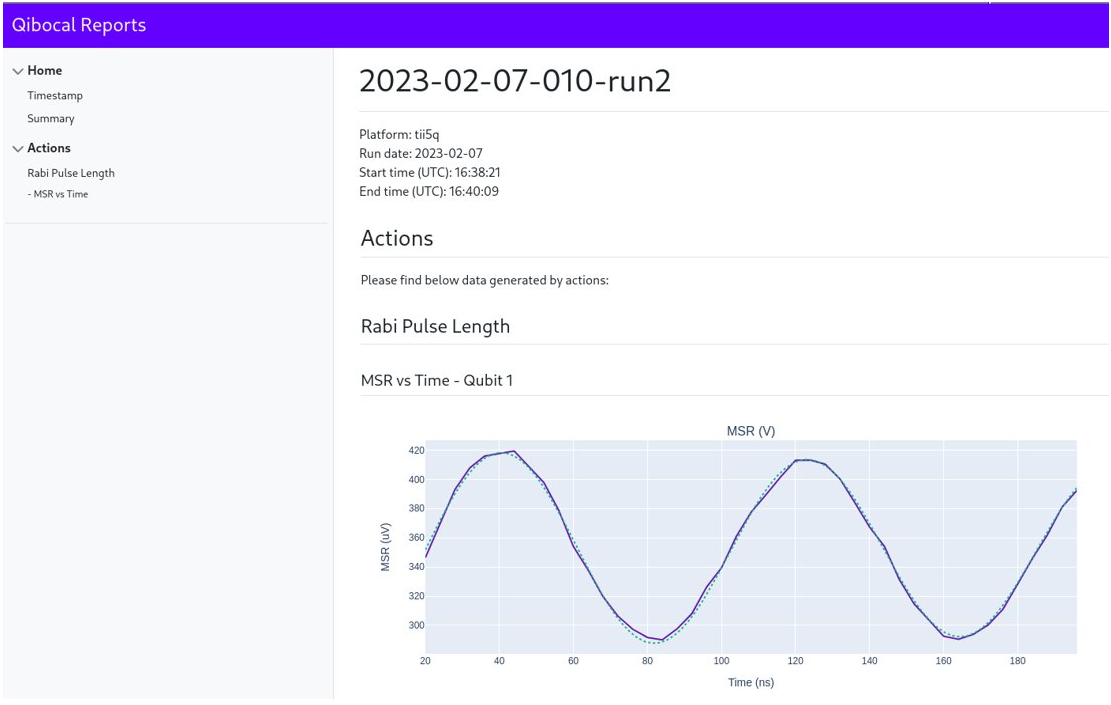
\includegraphics[width=\textwidth]{figures/qibocal_report.png}
     \end{figure}
   \end{columns}

 \end{frame}

 \begin{frame}{Benchmarking instruments performance \hfill \faBook\,\, \href{https://arxiv.org/abs/2308.06313}{arXiv:2308.06313}}

   We compare the ideal pulse sequence execution performance to instruments execution duration.
   \vspace{-0.5cm}
   \begin{figure}
     \includegraphics[height=6.5cm]{figures/routines.pdf}
   \end{figure}
   \vspace{-0.5cm}
   \begin{center}
     \small
     Zurich Instruments (ZI), Quantum Machines
     (QM), QBlox and RFSoC FPGA (Qibosoq+QICK).
   \end{center}

 \end{frame}

\section{Full-stack applications}

\begin{frame}[fragile]{Full-stack deployment: RB and Bell inequality \hfill \faBook\,\, \href{https://arxiv.org/abs/2308.06313}{arXiv:2308.06313}}
  Examples of results executed on quantum hardware (single-qubit) after calibration with Qibo:
  \begin{figure}
    \includegraphics[height=4.8cm]{figures/standard_rb.pdf}
    \includegraphics[height=4.8cm]{figures/bell_sweep_fig.pdf}
  \end{figure}
\end{frame}

\begin{frame}{Full-stack procedure: data regression \hfill \faBook\,\, \href{https://arxiv.org/abs/2308.06313}{arXiv:2308.06313}}

   \begin{columns}
     \column{6cm}
     \begin{block}{1. High-Level API (Qibo)}
       \begin{itemize}
         \item Define model prototype.
         \item Implement training loop.
         \item Perform training using simulation.
       \end{itemize}
     \end{block}
     \begin{exampleblock}{2. Calibration (Qibocal)}
     \begin{itemize}
       \item Calibrate qubit.
       \item Generate platform configuration.
     \end{itemize}
     \end{exampleblock}
     \begin{alertblock}{3. Execution (Qibolab)}
       \begin{itemize}
         \item Allocate calibrated platform.
         \item Compile and transpile circuit.
         \item Execute model and return results.
       \end{itemize}
     \end{alertblock}
     \column{6cm}
   \begin{figure}
     \includegraphics[width=\textwidth]{figures/qqpdf.pdf}
   \end{figure}
   \vspace{-0.3cm}
 \begin{table}
   \small
   \begin{tabular}{lc}
   \hline \hline
     \textbf{Parameter}     & \textbf{Value}  \\ \hline
     $N_{\rm data}$      & 50 points \\
     $N_{\rm shots}$ & 500 \\
     MSE & $10^{-3}$ \\
     Electronics & Xilinx ZCU216 \\
     Training time & $<1$h \\
   \hline \hline
   \end{tabular}
 \end{table}

   \end{columns}

 \end{frame}


\section{Outlook}

\begin{frame}{What next?}

  \vspace{0.5cm}
  \begin{columns}
    \column{8cm}
  Hands-on tutorials:
  \begin{enumerate}
    \item[1.] Setting up Qibo’s quantum middleware software environment, building quantum circuits.
    \item[2.] Quantum circuits, gates and shots. Bell states and ancillary qubits.
    \item[3.] Grover search algorithm.
    \item[4.] Introducing quantum noise and quantum hardware limitations
    \item[5.] Mitigating quantum noise via Quantum Error Mitigation
  \end{enumerate}

    \column{5cm}
    \begin{figure}
      \includegraphics[width=\textwidth]{figures/docs.png}
      {\color{blue}\url{https://qibo.science}}
    \end{figure}
  \end{columns}

\end{frame}

\begin{frame}
\centering
\Huge Let's code!
\begin{figure}
   \includegraphics[width=0.7\textwidth]{figures/hands_on.png}
\end{figure}
\end{frame}


\end{document}
